\documentclass[UTF8, 12pt]{report}

\usepackage{ctex}
\setCJKfamilyfont{xiukai}{FZSKBXKJW_0.ttf}
% \setCJKfamilyfont{songkeben}{FZQKBYSJW.ttf}
\newcommand{\xiukai}{\CJKfamily{xiukai}}
% \newcommand{\songkeben}{\CJKfamily{songkeben}}
\setCJKmainfont[BoldFont=SourceHanSerifSC-Bold.otf,ItalicFont=SourceHanSerifSC-Light.otf]{SourceHanSerifSC-Regular.otf}
\setCJKmonofont[BoldFont=SourceHanSansHWSC-Bold.otf,ItalicFont=SourceHanSansHWSC-Regular.otf]{SourceHanSansHWSC-Regular.otf}

\usepackage{amsfonts}
\usepackage{amsmath}
% \DeclareMathAlphabet{\mathpzc}{OMS}{cmsy}{m}{n}
\usepackage[scr=euler]{mathalfa}
\newcommand{\diff}{\mathrm{d}}
\newcommand{\euler}{\mathrm{e}}
\newcommand{\imag}{\mathrm{i}}
\newcommand{\image}{\mathrm{j}}

% \usepackage[siunitx]{circuitikz}
\usepackage{float}
\usepackage{graphicx}
\usepackage{fontspec}
\newfontfamily\perpetua[BoldFont=PERTIBD.ttf]{PERTILI.ttf}
% \newfontfamily\lucida[BoldFont=LCALLIG.ttf,ItalicFont=LCALLIG.ttf]{LCALLIG.ttf}
% \newfontfamily\xinshusong[BoldFont=FZXSSK.ttf,ItalicFont=FZXSSK.ttf]{FZXSSK.ttf}
% \newfontfamily\xiukai[BoldFont=FZSKBXKJW_0.ttf,ItalicFont=FZSKBXKJW_0.ttf]{FZSKBXKJW_0.ttf}
% \newfontfamily\songkeben[BoldFont=FZQKBYSJW.ttf,ItalicFont=FZQKBYSJW.ttf]{FZQKBYSJW.ttf}
% \newfontfamily\SourceHanSerifSC[BoldFont=SourceHanSerifSC-Bold.otf,ItalicFont=SourceHanSerifSC-Light.otf]{SourceHanSerifSC-Regular.otf}
% \newfontfamily\SourceHanSans[BoldFont=SourceHanSansHWSC-Bold.otf,ItalicFont=SourceHanSansHWSC-Regular.otf]{SourceHanSansHWSC-Regular.otf}
% \setCJKmainfont[BoldFont=SourceHanSerifSC-Bold.otf,ItalicFont=SourceHanSerifSC-Light.otf]{SourceHanSerifSC-Regular.otf}
% \setCJKmonofont[BoldFont=SourceHanSansHWSC-Bold.otf,ItalicFont=SourceHanSansHWSC-Regular.otf]{SourceHanSansHWSC-Regular.otf}

\usepackage{ntheorem}
\newtheorem{proposition}{命题}[section]
\newtheorem{theorem}{定理}[section]
\newtheorem{corollary}{推论}[section]
\newtheorem{lemma}{引理}[section]
\newtheorem{example}{例}[section]
\newtheorem*{proof}{证明:}[section]

\usepackage{geometry}
\geometry{a4paper,centering,top=3.0cm,bottom=3.0cm,left=2.1cm,right=2.1cm}

\usepackage{fancyhdr}
\pagestyle{fancy}
\renewcommand{\chaptermark}[1]{\markboth{第\chinese{chapter}章\ #1}{}}
\renewcommand{\sectionmark}[1]{\markright{#1}{}}

\fancypagestyle{main}{
    \fancyhf{}
    \setlength{\headheight}{27pt}
    \fancyhead[R]{\leftmark}
    \fancyhead[L]{\rightmark}
    \renewcommand{\headrulewidth}{0.4pt}
    \pagenumbering{arabic}
    \fancyfoot[C]{\thepage}
}

\usepackage[CJKbookmarks=true,hidelinks,unicode,psdextra]{hyperref}

\usepackage{titlesec}
\titleformat{\chapter}[display]{\raggedright\huge\bfseries}{第\chinese{chapter}章}{1em}{\Huge\vspace{1pt}}
\titleformat{\section}{\centering\Large\bfseries}{\S \arabic{section}}{1em}{}

\usepackage{enumerate}
\usepackage{enumitem}
\setlist[enumerate,1]{label=(\arabic*),font=\textup,
leftmargin=7mm,labelsep=1.5mm,topsep=0mm,itemsep=-0.8mm}
\setlist[enumerate,2]{label=\alph*),font=\textup,
leftmargin=7mm,labelsep=1.5mm,topsep=-0.8mm,itemsep=-0.8mm}

\newcommand{\romannum}[1]{\uppercase\expandafter{\romannumeral #1\relax}}
\def\ooint{{\bigcirc}\kern-11.5pt{\int}\kern-6.5pt{\int}}
\def\oooint{{\bigcirc}\kern-12.3pt{\int}\kern-7pt{\int}\kern-7pt{\int}}

\allowdisplaybreaks[3]

\title{\xiukai 数学习题集}
\author{\xiukai 李太吉}
\date{\xiukai 2019年8月9日}

\begin{document}

\begin{titlepage}

    \begin{center}

        \vspace*{6em}
        {\xiukai \Huge 数 \hspace{35pt} 学 \hspace{35pt} 习 \hspace{35pt} 题 \hspace{35pt} 集}\\
        \vspace*{15pt}
        {\perpetua \large The Collection of Mathematics Problems} \\
        \vspace*{\fill}
        {\xiukai \LARGE 李太吉 \ 编}\\
        \vspace*{25pt}
        {\xiukai \Large 2019年8月9日}\\

        \vspace*{\fill}
        \begin{figure}[H]
            \centering
            
\includegraphics[scale=0.2]{timg.jpg}
        \end{figure}
        {\large\textbf Copyright © 2019 - 2020 Li Taiji. All Rights Reserved.}

    \end{center}

\end{titlepage}

\pagestyle{main}
% \frontpagestyle
\tableofcontents

% \mainpagestyle

\chapter{数学分析}

\section{数列与极限}

\begin{proposition}[Cauthy命题]

    设$\{x_n\}$收敛于$l$,则它的前$n$项的算术平均数也收敛于$l$,即有
    $$\lim\limits_{x\to\infty}{\dfrac{x_1 + x_2 + \cdots + x_n}{n}} = l$$

\end{proposition}

\begin{proof}

    $\{x_n\}$收敛于$l$,则$\forall \varepsilon > 0$,$\exists N \in \mathbb{N}$,$n > N$ 时
    $$|x_n - l| < \varepsilon$$
    则

    \begin{align*}
        \left|\dfrac{x_1 + x_2 + \cdots + x_n}{n} - l\right| &= \left|\dfrac{\sum\limits_{i=1}^{n}{x_i - l}}{n}\right|\\
        &\leq \dfrac{\sum\limits_{i=1}^{n}{|x_i - l|}}{n}\\
        &= \dfrac{\sum\limits_{i=1}^{N}{|x_i - l|}}{n} + \dfrac{\sum\limits_{i=N+1}^{n}{|x_i - l|}}{n}\\
        &\leq \dfrac{M}{n} + \dfrac{(n-N)\varepsilon}{n}
    \end{align*}

    其中$M = \sum\limits_{i=1}^{N}{|x_i-l|}$,$M$为有限值。
    $N_1 = \max\left\{\left\lfloor\dfrac{M}{\varepsilon}\right\rfloor,\ N \right\}$,\\
    即有$n>N_1$时成立不等式
    $$\left| \dfrac{x_1 + x_2 + \cdots + x_n}{n} - l \right| < \varepsilon$$
    也即
    $$\lim\limits_{x\to\infty}{\dfrac{x_1 + x_2 + \cdots + x_n}{n}} = l$$

\end{proof}

\begin{corollary}[Cauthy命题推论]

    若$\lim\limits_{n\to\infty}{(a_n - a_{n-1})} = d$,
    则
    $$\lim\limits_{n\to\infty}{\dfrac{a_n}{n}} = d$$

\end{corollary}

\begin{proof}

    因为$\lim\limits_{n\to\infty}{(a_n - a_{n-1})} = d$,所以数列$\{a_n - a_{n - 1}\}$收敛于$d$。\\
    由\textup{Cauthy}命题知,
    
    \begin{align*}
        & \lim\limits_{n\to\infty}{\dfrac{(a_2 - a_1) + (a_3 - a_2) + \cdots + (a_{n + 1} - a_n)}{n}} \\
        = & \ \lim\limits_{n\to\infty}{\dfrac{a_{n + 1} - a_1}{n}} \\
        = & \ \lim\limits_{n\to\infty}{\dfrac{n + 1}{n} \dfrac{a_{n + 1}}{n + 1}} - \lim\limits_{n\to\infty}{\dfrac{a_1}{n}} = d
    \end{align*}

    即
    $$\lim\limits_{n\to\infty}{\dfrac{a_n}{n}} = d$$

\end{proof}

\begin{corollary}[Cauthy命题推论]

    设$\{a_n\}$是正数列,且收敛于$A$,
    则
    $$\lim\limits_{n\to\infty}{\sqrt[n]{a_1a_2\cdots a_n}} = A$$

\end{corollary}

\begin{proof}

    显然有
    $$\ln{\left((a_1a_2\cdots a_n)^{\frac{1}{n}}\right)} = \dfrac{\ln{a_1} + \ln{a_2} + \cdots + \ln{a_n}}{n}$$
    由\textup{Cauthy}命题知,因为$\{a_n\}$收敛于$A$,即数列$\{\ln{a_n}\}$收敛于$\ln{A}$,所以
    $$\lim\limits_{n\to\infty}{\dfrac{\ln{a_1} + \ln{a_2} + \cdots + \ln{a_n}}{n}} = \ln{A}$$
    也即
    $$\lim\limits_{n\to\infty}{\sqrt[n]{a_1a_2\cdots a_n}} = A$$

\end{proof}


\begin{corollary}[Cauthy命题推论]

    设$\{a_n\}$是正数列,且存在极限$\lim\limits_{n\to\infty}{\dfrac{a_{n+1}}{a_n}}=l$,
    则
    $$\lim\limits_{n\to\infty}{\sqrt[n]{a_n}} = l$$

\end{corollary}

\begin{proof}

    因为$\lim\limits_{n\to\infty}{\dfrac{a_{n+1}}{a_n}}=l$,所以数列$\left\{\ln{\dfrac{a_n}{a_{n - 1}}}\right\}$收敛于$\ln{l}$ \\
    由\textup{Cauthy}命题知,
    
    \begin{align*}
        & \lim\limits_{n\to\infty}{\dfrac{\ln{\dfrac{a_2}{a_1}} + \ln{\dfrac{a_3}{a_2}} + \cdots + \ln{\dfrac{a_{n + 1}}{a_n}}}{n}} \\
        = & \ \lim\limits_{n\to\infty}{\dfrac{\ln{\dfrac{a_{n + 1}}{a_1}}}{n}} \\
        = & \ \lim\limits_{n\to\infty}{\dfrac{\ln{a_{n + 1} - \ln{a_1}}}{n}} \\
        = & \ \lim\limits_{n\to\infty}{\dfrac{n + 1}{n}\dfrac{\ln{a_{n + 1}}}{n + 1}} - \lim\limits_{n\to\infty}{\dfrac{\ln{a_1}}{n}} = \ln{l}
    \end{align*}

    即
    $$\lim\limits_{n\to\infty}{\dfrac{\ln{a_n}}{n}} = \ln{l}$$
    也即
    $$\lim\limits_{n\to\infty}{\sqrt[n]{a_n}}=l$$

\end{proof}

\begin{proposition}[Cauthy命题$\infty$时的特例]

    $\lim\limits_{n\to\infty}{x_n} = +\infty$,证明:
    $$\lim\limits_{n\to\infty}{\dfrac{x_1 + x_2 + \cdots + x_n}{n}} = +\infty$$

\end{proposition}

\begin{proof} 

    $\forall A > 0$,由于$\lim\limits_{n\to\infty}{a_n} = +\infty$,故$\exists N_1 \in \mathbb{N}$,$n>N$时,$a_n > 2A + 2$,\\
    又
    $$\lim\limits_{n\to\infty}{\dfrac{n-N_1}{n}} = 1 > \dfrac{1}{2}$$
    $$\lim\limits_{n\to\infty}{\dfrac{x_1 + x_2 + \cdots + x_n}{n}} = 0 > -1$$
    于是

    \begin{align*}
        \dfrac{x_1 + x_2 + \cdots + x_n}{n} & = \dfrac{x_1 + x_2 + \cdots + x_{N_1}}{n} + \dfrac{x_{N_1+1} + x_{N_1+2} + \cdots + x_n}{n} \\
        & > -1 + \dfrac{n-N_1}{n}(2A+2) \\
        & > -1 + \dfrac{1}{2}(2A + 2) \\
        & = A 
    \end{align*}

    故
    $$\lim\limits_{n\to\infty}{\dfrac{x_1 + x_2 + \cdots + x_n}{n}} = +\infty$$
    
\end{proof} 

\begin{proposition}[$\dfrac{0}{0}$型的stolz公式]

    设$\{a_n\}$和$\{b_n\}$都是收敛于$0$的数列,其中$\{a_n\}$是严格单调递减数列,且存在
    $$\lim\limits_{n\to\infty}{\dfrac{b_{n+1}- b_n}{a_{n+1}-a_n}} = l $$
    其中$l$为有限值或无穷。则有
    $$\lim\limits_{n\to\infty}{\dfrac{b_n}{a_n}} = l$$

\end{proposition}

\begin{proof}
    
    $\forall \varepsilon>0$,$\exists N \in \mathbb{N}$,$n > N$时
    $$\left| \dfrac{b_n-b_{n+1}}{a_n-a_{n+1}}-l\right| < \varepsilon$$
    $$(l-\varepsilon)(a_n-a_{n+1})<b_n-b_{n+1}<(l+\varepsilon)(a_n-a_{n+1})$$
    任取$m>n$,将上式中$n$替换为$n+1$,$n+2$,$n+3$,$\cdots$,$m-1$,有

    \begin{align*}
        &(l-\varepsilon)(a_{n+1}-a_{n+2})<b_{n+1}-b_{n+2}<(l+\varepsilon)(a_{n+1}-a_{n+2})\\
        &(l-\varepsilon)(a_{n+2}-a_{n+3})<b_{n+2}-b_{n+3}<(l+\varepsilon)(a_{n+2}-a_{n+3})\\
        &\vdots\\
        &(l-\varepsilon)(a_{m-1}-a_{m})<b_{m-1}-b_{m}<(l+\varepsilon)(a_{m-1}-a_{m})
    \end{align*}

    将上式相加得到
    $$(l-\varepsilon)(a_{n}-a_{m})<b_{n}-b_{m}<(l+\varepsilon)(a_{n}-a_{m})$$
    $$\left| \dfrac{b_n-b_{m}}{a_n-a_{m}}-l\right| < \varepsilon$$
    对于$m$,令$m\to+\infty$,有
    $$\lim\limits_{m\to\infty}{a_m}=\lim\limits_{m\to\infty}{b_m}=0$$
    又
    $$\lim\limits_{m\to\infty}{\left| \dfrac{b_n-b_{m}}{a_n-a_{m}}-l\right|} = \left|\dfrac{b_n}{a_n}-l\right|$$
    则
    $$\lim\limits_{n\to\infty}{\dfrac{b_n}{a_n}} = l$$

\end{proof}

\begin{proposition}[$\dfrac{*}{\infty}$型的stolz公式]
    
    设有数列$\{a_n\}$和$\{b_n\}$,其中$\{a_n\}$是严格单调增加的发散数列,且存在
    $$\lim\limits_{n\to\infty}{\dfrac{b_{n+1}- b_n}{a_{n+1}-a_n}} = l $$
    其中$l$为有限值或无穷。则有
    $$\lim\limits_{n\to\infty}{\dfrac{b_n}{a_n}} = l$$

\end{proposition}

\begin{proof}

    \begin{enumerate}

        \item
            $l$为有限值\\
            $\forall \varepsilon>0$,$\exists N \in \mathbb{N}$,$n > N$时
            $$\left| \dfrac{b_n-b_{n+1}}{a_n-a_{n+1}}-l\right| < \varepsilon$$
            $$(l-\varepsilon)(a_n-a_{n+1})<b_n-b_{n+1}<(l+\varepsilon)(a_n-a_{n+1})$$
            取定$n$,将上式中$n$替换为$N$,$N+1$,$N+2$,$\cdots$,$n-1$,有

            \begin{align*}
                &(l-\varepsilon)(a_{N}-a_{N+1})<b_{N}-b_{N+1}<(l+\varepsilon)(a_{N}-a_{N+1})\\
                &(l-\varepsilon)(a_{N+1}-a_{N+2})<b_{N+1}-b_{N+2}<(l+\varepsilon)(a_{N+1}-a_{N+2})\\
                &\vdots\\
                &(l-\varepsilon)(a_{n-1}-a_{n})<b_{n}-b_{n}<(l+\varepsilon)(a_{n-1}-a_{n})
            \end{align*}

            将上式相加得到
            $$(l-\varepsilon)(a_{n}-a_{N})<b_{n}-b_{N}<(l+\varepsilon)(a_{n}-a_{N})$$
            $$\left| \dfrac{b_n-b_{N}}{a_n-a_{N}}-l\right| < \varepsilon$$
            $$\dfrac{b_n}{a_n}-l = \left(1-\dfrac{a_N}{a_n}\right)\left(\dfrac{b_n-b_N}{a_n-a_N}-l\right) + \dfrac{b_N-la_N}{a_N}$$
            由于$\lim\limits_{n\to\infty}{a_n} = +\infty$,$\exists N_1 \in \mathbb{N}$,使得当$n>N_1$时成立
            $$0<1-\dfrac{a_N}{a_n}<2$$
            $$\left|\dfrac{b_N-la_N}{a_n}\right|<\varepsilon$$
            则当$n>\max\{N_1, N\}$有
            $$\left|\dfrac{b_n}{a_n}-l\right|<3\varepsilon$$

        \item
            $l$为$+\infty$时\\
            $\forall \varepsilon>0$,$\exists N \in \mathbb{N}$,$n > N$时
            $$b_{n+1}-b_n>a_{n+1}-a_n$$
            由\textup{(1)}可知,
            $$b_{n+1}-b_N>a_{n+1}-a_n$$
            则$\lim\limits_{n\to\infty}{b_n}=+\infty$,且$\{b_n\}$严格单调增加,
            所以,
            $$\lim\limits_{n\to\infty}{\dfrac{b_n}{a_n}}=\lim\limits_{n\to\infty}{\dfrac{a_n-a_{n-1}}{b_n-b_{n-1}}} = 0$$
            故
            $$\lim\limits_{n\to\infty}{\dfrac{b_n}{a_n}}=\lim\limits_{n\to\infty}{\dfrac{\frac{1}{a_n}}{b_n}}=+\infty$$

        \item $l$为$-\infty$时同\textup{(2)}.

    \end{enumerate}

\end{proof}

\begin{proposition}[Carleman不等式]

    设$\sum\limits_{n=1}^{\infty}{a_n}$为收敛的正项级数,
    则不等式
    $$\sum\limits_{n=1}^{\infty}{\sqrt[n]{a_1a_2\cdots a_n}}\leq \euler\sum\limits_{n=1}^{\infty}{a_n}$$

\end{proposition}

\begin{proof}

    \begin{align*}
        \sum\limits_{n=1}^{\infty}{\sqrt[n]{a_1a_2\cdots a_n}} &= \sum\limits_{n=1}^{\infty}{\dfrac{\sqrt[n]{a_1(2a_2)\cdots (na_n)}}{\sqrt[n]{n!}}}\\
        &\leq\sum\limits_{n=1}^{\infty}{\dfrac{a_1+2a_2+\cdots +na_n}{n\sqrt[n]{n!}}}\\
        &\leq\euler\sum\limits_{n=1}^{\infty}{\dfrac{a_1+2a_2+\cdots +na_n}{n(n+1)}}\\
        &=\euler\sum\limits_{n=1}^{\infty}{\dfrac{1}{n(n+1)}\sum\limits_{k=1}^{n}{ka_k}}\\
        &=\euler\sum\limits_{k=1}^{N}{\left\{ka_k\left[\sum\limits_{n=k}^{N}{\dfrac{1}{n(n+1)}}\right]\right\}}\\
        &=\euler\sum\limits_{k=1}^{N}{ka_k(\dfrac{1}{k}-\dfrac{1}{N + 1})} \\
        &\leq\euler\sum\limits_{k=1}^{N}{a_k}
    \end{align*}

    令$N\to+\infty$,即可得到\textup{Carleman}不等式。\\
    下证不等式右边的系数$\euler$不能在改进。\\
    对于每个$N$构造一个数列
    $$b_n=\left\{
        \begin{aligned}
            &\dfrac{1}{n}, & n & = 1,2,\cdots,N \\
            &0, & n & > N
        \end{aligned}
    \right.
    $$
    然后作出两个级数和之比,令$n\to+\infty$,应用\textup{stolz}定理,有
    $$\lim\limits_{N\to\infty}{\dfrac{\sum\limits_{n=1}^{N}{\sqrt[n]{a_1a_2\cdots a_n}}}{\sum\limits_{n=1}^{N}{b_n}}}=\lim\limits_{N\to\infty}{\dfrac{N}{\sqrt[N]{N!}}}=\euler$$

\end{proof}

\begin{theorem}[Sapagof判别法]

设正数列$\{a_n\}$单调减少,则$\lim\limits_{n\to\infty}{a_n}=0$的充分必要条件是正项级数$\sum\limits_{n=1}^{\infty}{(1-\dfrac{a_{n+1}}{a_n})}$发散。
    
\end{theorem}

\begin{proof}
    
    先证充分性。\\
    正数列$\{a_n\}$单调减少,则$\{a_n\}$存在极限,即
    $$\lim\limits_{n\to\infty}{a_n} = a(a>0)$$
    设$b_n=1-\dfrac{a_{n+1}}{a_n} = \dfrac{a_n-a_{n+1}}{a_n}\leq\dfrac{a_n-a_{n+1}}{a}$,
    则

    \begin{align*}
        \sum\limits_{n=1}^{m}{b_n}&=\sum\limits_{n=1}^{m}{(1-\dfrac{a_{n+1}}{a_{n}})}\\
        &\leq\dfrac{1}{a}\sum\limits_{n=1}^{m}{(a_n-a_{n+1})}\\
        &=\dfrac{1}{a}(a_1-a_{m+1})
    \end{align*}

    \begin{align*}
        \sum\limits_{n=1}^{\infty}{b_n} &= \lim\limits_{m\to\infty}{\sum\limits_{n=1}^{m}{b_n}}\\
        &\leq\lim\limits_{m\to\infty}{\dfrac{1}{a}(a_1-a_{m+1})}\\
        & = \dfrac{1}{a}(a_1-a)
    \end{align*}

    可知$\sum\limits_{n=1}^{\infty}{b_n}$收敛。\\
    再证必要性。若$a=0$,则由柯西准则,

    \begin{align*}
        \sum\limits_{k=n+1}^{n+p}{b_k} &= \sum\limits_{k=n+1}^{n+p}{(1-\dfrac{a_{k+1}}{a_k})}\\
        &\geq\sum\limits_{k=n+1}^{n+p}{\dfrac{a_k-a_{k+1}}{a_k}}\\
        & = \dfrac{1}{a_{n+1}}(a_{n+1}-a_{n+p+1})\\
        & = \dfrac{a_{n+p+1}}{a_{n+1}}
    \end{align*}

    因为$\lim\limits_{n\to\infty}{a_n}=0$,则总存在$p \in \mathbb{N}$,
    使得
    $$\sum\limits_{k=n+1}^{n+p}{b_k}\geq\dfrac{1}{2}$$
    所以$\sum\limits_{n=1}^{\infty}{b_n}$发散。

\end{proof}

\begin{theorem}[Sapagof判别法等价形式\romannum{1}]

    设$\{a_n\}$是单调增加的正数列,则该数列与级数
    $$\sum\limits_{n=1}^{\infty}{\left(1-\dfrac{a_{n+1}}{a_n}\right)}$$
    同敛散。
        
\end{theorem}

\begin{proof}

    $\{a_n\}$单调增加,若$\{a_n\}$收敛,则
    $$\lim\limits_{n\to\infty}{a_n}=a \ (a\neq+\infty)$$

    \begin{align*}
        \sum\limits_{k=n+1}^{n+p}{b_k} &= \sum\limits_{k=n+1}^{n+p}{(1-\dfrac{a_k}{a_{k+1}})}\\
        & \leq \sum\limits_{k=n+1}^{n+p}{\dfrac{a_{k+1}-a_k}{a_{n+1}}}\\
        & = \dfrac{a_{n+p+1}-a_{n+1}}{a_{n+1}}
    \end{align*}

    因为$\lim\limits_{n\to\infty}{a_n}=a$,则$\forall \varepsilon >0$,$\exists N\in \mathbb{N}$,$n>N$时,
    $$|a_n-a|<\varepsilon$$
    所以

    \begin{align*}
        \left| \dfrac{a_{n+p+1}-a_{n+1}}{a_{n+1}}\right| &= \left| \dfrac{a_{n+p+1}-a + a -a_{n+1}}{a_{n+1}}\right|\\
        & = \dfrac{|a_{n+p+1}-a|+|a_{n+1}-a|}{a_{n+1}}\\
        & = \dfrac{2\varepsilon}{a_{n+1}}
    \end{align*} 

    所以$\sum\limits_{n=1}^{\infty}{b_n}$收敛。\\
    若$\lim\limits_{n\to\infty}{a_n}=+\infty$,则

    \begin{align*}
        \sum\limits_{k=n+1}^{n+p}{b_k} &= \sum\limits_{k=n+1}^{n+p}{(1-\dfrac{a_k}{a_{k+1}})}\\
        & \leq \sum\limits_{k=n+1}^{n+p}{\dfrac{a_{k+1}-a_k}{a_{n+p+1}}}\\
        & = \dfrac{a_{n+p+1}-a_{n+1}}{a_{n+p+1}}\\
        & = 1-\dfrac{a_{n+1}}{a_{n+p+1}}
    \end{align*}

    由柯西准则,因为$\lim\limits_{n\to\infty}{a_n}=+\infty$,则存在$p \in \mathbb{N}$,
    $$ \dfrac{a_{n+1}}{a_{n+p+1}} \leq \dfrac{1}{2}$$
    则
    $$ 1-\dfrac{a_{n+1}}{a_{n+p+1}} \geq \dfrac{1}{2}$$
    所以$\sum\limits_{n=1}^{\infty}{b_n}$发散。

\end{proof}

\begin{theorem}
    
    $\{S_n\}$是正项级数$\sum\limits_{n=1}^{\infty}{a_n}$的部分和数列,则
    $\sum\limits_{n=1}^{\infty}{a_n}$和$\sum\limits_{n=1}^{\infty}{\dfrac{a_n}{S_n}}$同敛散。

\end{theorem}

\begin{proof}
    
    $\sum\limits_{n=1}^{\infty}{a_n}$收敛,则

    \begin{align*}
        \sum\limits_{k=n+1}^{n+p}{\dfrac{a_k}{S_k}} & \leq \sum\limits_{k=n+1}^{n+p}{\dfrac{a_k}{S_{n+1}}}\\
        &\leq \dfrac{S_{n+p+1}-S_{n}}{S_{n+1}}\\
        &\leq \dfrac{S_{n+p+1}-S_{n}}{S_{n}}
    \end{align*}

    设$\sum\limits_{n=1}^{\infty}{a_n} = S$,则$\forall \varepsilon >0$,$\exists N\in\mathbb{N}$,$n>N$时,
    $$|S_n-S|<\varepsilon$$

    \begin{align*}
        \left|\dfrac{S_{n+p+1}-S_{n}}{S_{n}}\right| &= \left|\dfrac{S_{n+p+1}-S+S-S_{n}}{S_{n}}\right|\\
        & \leq \dfrac{|S_{n+p+1}-S|+|S_{n+1}-S|}{S_n}\\
        & = \dfrac{2\varepsilon}{S_n}
    \end{align*}

    所以$\sum\limits_{n=1}^{\infty}{\dfrac{a_n}{S_n}}$收敛。\\
    $\sum\limits_{n=1}^{\infty}{a_n}$发散,则$\lim\limits_{n\to\infty}{\sum\limits_{k=1}^{n}{a_k}}=+\infty$,且有

    \begin{align*}
        \sum\limits_{k=n+1}^{n+p}{\dfrac{a_k}{S_k}} & \geq \sum\limits_{k=n+1}^{n+p}{\dfrac{a_k}{S_{n+p+1}}}\\
        &\geq \dfrac{S_{n+p+1}-S_{n}}{S_{n+p+1}}\\
        &= 1-\dfrac{S_{n}}{S_{n+p+1}}
    \end{align*}

    因为$\lim\limits_{n\to\infty}{\sum\limits_{k=1}^{n}{a_k}}=+\infty=\lim\limits_{n\to\infty}{S_n}=+\infty$,则存在$p\in\mathbb{N}$,
    $$1-\dfrac{S_{n}}{S_{n+p+1}} \geq \dfrac{1}{2}$$
    所以$\sum\limits_{n=1}^{\infty}{\dfrac{a_n}{S_n}}$发散。

\end{proof}

\begin{theorem}
    
    \begin{enumerate}

        \item 
            正项级数$\sum\limits_{n=1}^{\infty}{a_n}$收敛的充分必要条件时存在正数列$\{b_n\}$和正数$\delta$,使得当$n$充分大时有
            $$b_n \cdot \dfrac{a_n}{a_{n+1}}-b_{n+1}\geq \delta >0$$

        \item 
            正项级数$\sum\limits_{n=1}^{\infty}{a_n}$发散的充分必要条件时存在发散的正项级数$\sum\limits_{n=1}^{\infty}{\dfrac{1}{b_n}}$,使得当$n$充分大时有
            $$b_n  \cdot \dfrac{a_n}{a_{n+1}}-b_{n+1}\leq0$$

    \end{enumerate}

\end{theorem}

\begin{proof}
    
    \begin{enumerate}

        \item   
            先证充分性。\\
            由$b_n \cdot \dfrac{a_n}{a_{n+1}}-b_{n+1}\geq \delta >0$得
            $$a_nb_n-a_{n+1}b_{n+1}\geq \delta a_{n+1}$$
            $$a_{n+1}\leq \dfrac{1}{\delta}(a_nb_n-a_{n+1}b_{n+1})$$
            不妨设$n\geq 1$,时上式成立,则

            \begin{align*}
                \sum\limits_{k=1}^{n}{a_k} &= a_1 + \sum\limits_{k=2}^{n}{a_k}\\
                & \leq a_1 +  \dfrac{1}{\delta}\sum\limits_{k=1}^{n-1}{(a_k b_k-a_{k+1}b_{k+1})}\\
                & = a_1 +  \dfrac{1}{\delta}(a_1 b_1-a_{n}b_{n})\\
                & = a_1 +  \dfrac{1}{\delta}a_1 b_1
            \end{align*}

            所以$\sum\limits_{n=1}^{\infty}{a_n}$收敛。
            再证必要性。\\
            令
            $$b_n=\dfrac{R_n}{a_n}$$
            其中$R_n$为$\sum\limits_{n=1}^{\infty}{a_n}$的余项,即
            $$R_n= S-S_n$$
            $$b_n \cdot \dfrac{a_n}{a_{n+1}}-b_{n+1}=\dfrac{R_n}{a_{n+1}}-\dfrac{R_{n+1}}{a_{n+1}}=1>0$$
            必要性得证。

        \item   
            充分性即为比较判别法的比值形式。\\
            下证必要性。\\
            令
            $$b_n=\dfrac{S_n}{a_n}$$
            易知$\sum\limits_{n=1}^{\infty}{\dfrac{1}{b_n}}$发散
            $$b_n \cdot \dfrac{a_n}{a_{n+1}}-b_{n+1}=\dfrac{S_{n}-S_{n+1}}{a_{n+1}}=-1\leq0$$
            必要性得证。

\end{enumerate}

\end{proof}

\begin{proposition}
    
    $\lim\limits_{n\to\infty}{(a_{n+p} - a_n)} = \lambda_1$,$p$为固定的正整数,$\lambda$是常数,则
    $$\lim\limits_{n\to\infty}{\dfrac{a_n}{\lambda}} = \dfrac{\lambda}{p}$$

\end{proposition}

\begin{proof}
    
    对固定的$i \in \mathbb{N}$,$\{a_{np + i}\}$是$\{a_{n}\}$的子列\\
    由$\lim\limits_{n\to\infty}{a_{n+p} - a_n} = \lambda$,则
    $$\lim\limits_{n\to\infty}{a_{(n+1)p + i} - a_{np+i}} = \lambda$$
    令$A^{(i)}_{n} = a_{(n+1)p+i} - a_{np + i}$,由\textup{Cauthy}命题知
    $$\lim\limits_{n\to\infty}{\dfrac{A_1 + A_2 + \cdot + A_n}{n}} = \lambda$$
    即
    $$\lim\limits_{n\to\infty}{\dfrac{a_{(n+1)p+i} - a_{p+i}}{n}} = \lim\limits_{n\to\infty}{\dfrac{a_{(n+1)p+i}}{n}} = \lambda$$
    则
    $$\lim\limits_{n\to\infty}{\dfrac{a_n}{n}} = \lim\limits_{n\to\infty}{\dfrac{a_{np+i}}{np+i}} = \dfrac{n}{np+i} \lim\limits_{n\to\infty}{\dfrac{a_{np+i}}{n}} = \dfrac{\lambda}{p}$$

\end{proof}

\begin{proposition}

    将二项式系数$\binom{n}{0}$,$\binom{n}{1}$,$\cdots$,$\binom{n}{n}$的算术平均数和几何平均数分别记作$A_n$和$G_n$. 证明:

    \begin{enumerate}

        \item $$\lim\limits_{n\to\infty}{\sqrt[n]{A_n}} = 2$$
                
        \item $$\lim\limits_{n\to\infty}{\sqrt[n]{G_n}} = \euler^{\frac{1}{2}}$$

    \end{enumerate}

\end{proposition}

\begin{proof}

    \begin{enumerate}
        
        \item 
            因为$$A_n = \sum\limits_{k=0}^{n}{\binom{n}{k}} = 2^n$$则
            $$\lim\limits_{n\to\infty}{\sqrt[n]{A_n}} = \lim\limits_{n\to\infty}{\sqrt[n]{\dfrac{2^n}{n}}} = 2$$

        \item 
            因为$$G_n = \sqrt[n]{\binom{n}{0}\binom{n}{1}\cdots\binom{n}{n}}$$则
            $$\lim\limits_{n\to\infty}{\sqrt[n]{G_n}}  = \lim\limits_{n\to\infty}{\sqrt[n^2]{\binom{n}{0}\binom{n}{1}\cdots\binom{n}{n}}} = \lim\limits_{n\to\infty}{\dfrac{1}{n^2} \sum\limits_{k=0}^{n}{\ln{\binom{n}{k}}}} = \euler^{\frac{1}{2}}  $$
    
        \end{enumerate}
    
\end{proof}

\begin{proposition}
    
    设$x_n = \dfrac{1}{n^2} \sum\limits_{k=0}^{n}{\ln{\binom{n}{k}}},\ n\in\mathbb{N}$,求$\lim\limits_{n\to\infty}{x_n}$

\end{proposition}

\begin{proof}
    
    应用\textup{stolz}公式,知

    \begin{align*}
        \lim\limits_{n\to\infty}{x_n}  = & \lim\limits_{n\to\infty}{\dfrac{\sum\limits_{k=0}^{n}{\ln{\binom{n+1}{k}}} - \sum\limits_{k=0}^{n}{\ln{\binom{n}{k}}}}{(n+1)^2 - n^2}} \\
        = & \lim\limits_{n\to\infty}{\dfrac{\sum\limits_{k=0}^{n}{\ln{\dfrac{n+1}{n+1-k}}}}{2n+1}} \\
        = & \lim\limits_{n\to\infty}{\dfrac{\ln{(1+\frac{1}{n})^{n-1}}}{2}} \\
        = & \dfrac{1}{2}
    \end{align*}

\end{proof}

\begin{proposition}
    
    设数列$\{a_n\}$满足$\lim\limits_{n\to\infty}{a_n\sum\limits_{k=1}^{n}{a_k^2}} = 1$,证明:
    $$\lim\limits_{n\to\infty}{\sqrt{3na_n}} = 1$$

\end{proposition}

\begin{proof}

    令$S_n = \sum\limits_{k=1}^{n}{a_k^2}$,则$S_n$单调增加,且$S_n\to\infty$,否则若$\lim\limits_{n\to\infty}{S_n} = S$,\\
    则$\lim\limits_{n\to\infty}{a_n^2} = 0$,即
    $$\lim\limits_{n\to\infty}{a_n} = 0$$
    所以
    $$\lim\limits_{n\to\infty}{a_nS_n} = \lim\limits_{n\to\infty}{a_nS} = 0$$
    与题设矛盾。故$\lim\limits_{n\to\infty}{S_n} = +\infty$,又
    $$\lim\limits_{n\to\infty}{a_n} = \lim\limits_{n\to\infty}{a_n \cdot S_n \cdot \dfrac{1}{S_n}} = \lim\limits_{n\to\infty}{a_nS_n} \cdot \lim\limits_{n\to\infty}{\dfrac{1}{S_n}} = 0$$

    \begin{align*}
        S_n^3 - S_{n-1}^3 &= (S_n - S_{n-1}) (S_n^2 + S_{n-1}S_n + S_{n-1}^2) \\
        = & a_n^2 (2S_n^2 - 3a_n^2S_n + a_n^4) \\
        = & 2a_n^2S_n^2 - 3a_n^4S_n + a_n^6 
    \end{align*}
    
    $$\lim\limits_{n\to\infty}{S_n^3 - S_{n-1}^3}= \lim\limits_{n\to\infty}{\big( 3(a_nS_n)^2 - 3a_n^3(a_nS_n) + a_n^6 \big)} = 3$$
    $$\lim\limits_{n\to\infty}{\dfrac{1}{3na_n^3}} = \lim\limits_{n\to\infty}{\dfrac{1}{a_n^3S_n^3} \cdot \dfrac{S_n^3}{3n}} = \lim\limits_{n\to\infty}{\dfrac{S_n^3}{3n}} = \lim\limits_{n\to\infty}{\dfrac{S_n^3 - S_{n-1}^3}{3}} = 1$$
    故
    $$\lim\limits_{n\to\infty}{\sqrt{3na_n}} = 1$$

\end{proof}

\begin{proposition}

    $\lim\limits_{n\to\infty}{a_n} = a $,$\lim\limits_{n\to\infty}{b_n} = b $,证明:
    $$\lim\limits_{n\to\infty}{\dfrac{a_0b_n + a_1b_{n-1} + \cdots + a_nb_0}{n}} = ab$$

\end{proposition}

\begin{proof}

    因$\lim\limits_{n\to\infty}{a_n} = a$,$\lim\limits_{n\to\infty}{b_n} = b $,故数列$\{a_n\},\ \{b_n\}$有界,\\
    $\exists M > 0$,
    $$|a_n| < M,\quad |b_n| < M, \quad \forall n \in \mathbb{N}$$
    $\forall \varepsilon > 0 $,$\exists N \in \mathbb{N}$,$n > N$时有
    $$|a_n -a| < \dfrac{\varepsilon}{4M}, \quad |b_n -b| < \dfrac{\varepsilon}{4M}$$
    取自然数$N_1 > \max\left\{N,\ \dfrac{2M}{\varepsilon}\left( \sum\limits_{k=0}^{n}{|a_k - a|} + \sum\limits_{k=0}^{n}{(|b_k - a|)} + |b| \right)\right\}$\\
    则当$n > N_1$时有

    \begin{align*}
        &\left| \dfrac{a_0b_n + a_1b_{n-1} + \cdots + a_nb_0}{n} \right| \\
        = \ & \dfrac{1}{n} \left| \sum\limits_{k=0}^{n}{b_{n-k}(a_k - a)} + \sum\limits_{k=0}^{n}{a_k(b_{n-k} - b)} + ab \right| \\
        = \ & \dfrac{M}{N} \left| \sum\limits_{k=0}^{N_1}{|a_k - a|} + \sum\limits_{k=0}^{N_1}{|b_{n-k} - b|} + |b| \right| \\
        \ & + \ \dfrac{M}{n} \left| \sum\limits_{k=N_1+1}^{n}{|a_k - a|} + \sum\limits_{k=N_1}^{n}{|b_{n-k} - b|} \right| \\
        \leq \ & \dfrac{\varepsilon}{2} + \dfrac{2M}{n}(n - N_1) - \dfrac{\varepsilon}{4M} \\
        < \ & \varepsilon 
    \end{align*}

    故
    $$\lim\limits_{n\to\infty}{\dfrac{a_0b_n + a_1b_{n-1} + \cdots + a_nb_0}{n}} = ab$$
    
\end{proof}

\begin{proposition}

    设$a_1 = 1$,$a_n = n(a_{n-1}+1),\quad n = 2,3,\cdots $,且
    $$x_n = \prod_{k=1}^{n}{\left(1+\dfrac{1}{a_n}\right)}$$
    求$\lim\limits_{n\to\infty}{x_n}$

\end{proposition}

\begin{proof}

    由$\dfrac{a_{n-1}+1}{a_n} = \dfrac{1}{n}$得

    \begin{align*}
        \prod_{k=1}^{n}{\left(1+\dfrac{1}{a_n}\right)} = & \left(1+\dfrac{1}{a_1}\right) \left(1+\dfrac{1}{a_2}\right) \cdots \left(1+\dfrac{1}{a_n}\right) \\
        = & \dfrac{a_1 + 1}{a_1} \cdot \dfrac{a_2 + 1}{a_2} \cdots \dfrac{a_n + 1}{a_n} \\
        = & \dfrac{1}{a_1} \cdot \dfrac{a_1 + 1}{a_2} \cdot \dfrac{a_2 + 1}{a_3} \cdots \dfrac{a_{n-1} + 1}{a_n} \cdot a_{n+1} \\
        = & \dfrac{1}{1} \cdot \dfrac{1}{2} \cdots \dfrac{1}{n} \\
        = &\dfrac{a_{n+1}}{n!} 
    \end{align*}

    \begin{align*}
        \dfrac{a_n}{n!} = & \dfrac{n(a_{n-1}+1)}{n!} = \dfrac{a_{n-1}}{(n-1)!} + \dfrac{1}{(n-1)!} \\
        = & \dfrac{a_{n-2}}{(n-2)!} + \dfrac{1}{(n-2)!} + \dfrac{1}{(n-1)!} \\
        & \cdots \\ 
        = & \dfrac{a_1}{1!} + \dfrac{1}{1!} + \dfrac{1}{2!} + \cdots + \dfrac{1}{(n-1)!} \\
        = & \sum\limits_{k=1}^{n-1}{\dfrac{1}{k!}} 
    \end{align*}

    则
    $$\dfrac{a_n}{n!} = \sum\limits_{k=1}^{n}{\dfrac{1}{k!}}$$
    所以
    $$\lim\limits_{n\to\infty}{x_n} = \lim\limits_{n\infty}{\sum\limits_{k=0}^{n}{\dfrac{1}{k!}}} = \euler$$

\end{proof}

\begin{proposition}

    设$a_1,a_2>0$,$a_{n+1} = \dfrac{2}{a_n + a_{n-1}}$,证明:$\{a_n\}$收敛。

\end{proposition}

\begin{proof}

    选取$\alpha$,使得
    $$\alpha < \min\{a_0,a_1\} \leq \max\{a_0,a_1\} < \dfrac{1}{\alpha}$$
    由数学归纳法可证
    $$\alpha < \min\{a_{n-1},a_n\} \leq \max\{a_{n-1},a_n\} < \dfrac{1}{\alpha}$$
    即
    $$\alpha < a_n < \dfrac{1}{\alpha},\quad \forall n\in\mathbb{N}$$
    所以$\{a_n\}$有界\\
    令
    $$L = \limsup_{n\to\infty}{a_n},\quad l = \liminf_{n\to\infty}{a_n}$$
    且易知$L,l$均是有限数,则$L \leq \dfrac{1}{\alpha},\quad l \geq \alpha$
    \begin{align*}
        L & = \limsup_{n\to\infty}{a_n} = \limsup_{n\to\infty}{\dfrac{2}{a_{n-1} + a_{n-2}}} \\
         & = \dfrac{1}{\liminf\limits_{n\to\infty}{(a_{n-1} + a_{n-2})}} = \dfrac{2}{\liminf\limits_{n\to\infty}{a_{n-1}} + \liminf\limits_{n\to\infty}{a_{n-2}}} \\ 
         &= \dfrac{1}{l}
    \end{align*}
    同理$l = \dfrac{1}{L}$,则$lL = 1$\\
    可设$\{a_{nk+3}\}$收敛到$L$,$\{a_{nk+2}\},\{a_{nk+1}\},\{a_{nk}\}$分别收敛到$a,b,c$,则$l < a,b,c < L$,又\\
    $L = \dfrac{2}{a+b} $,则$a+b = 2l $,同理,$b =c =L$\\
    所以$l = L = 1$,$\{a_n\}$收敛,极限为$1$。

\end{proof}

\begin{proposition}

    证明:数列$x_n = \dfrac{1}{1+1} + \dfrac{1}{2 + \frac{1}{2}} + \cdots + \dfrac{1}{n+\frac{1}{n}} - \ln{\dfrac{n}{\sqrt{2}}} \quad (n = 1,2,\cdots)$\\
    有位于$\left[0,\dfrac{1}{2}\right]$的极限。
    
\end{proposition}

\begin{proof}

    设
    $$f(x) = \dfrac{1}{x + \frac{1}{x}} = \dfrac{x}{x^2 + 1}$$
    则
    $$f'(x) = \dfrac{1-x^2}{(x^2 + 1)^2} < 1,\quad x\in[1,+\infty)$$
    所以$f(x)$在$[1,+\infty)$上单调减少。

    \begin{align*}
        x_n \geq & \int_{1}^{2}{\dfrac{1}{x+\frac{1}{x}}}\diff x + \int_{2}^{3}{\dfrac{1}{x+\frac{1}{x}}}\diff x + \cdots + \int_{2}^{3}{\dfrac{1}{x+\frac{1}{x}}}\diff x - \ln{\dfrac{n}{\sqrt{2}}} \\
        = & \int_{1}^{n+1}{\dfrac{x}{x^2 + 1}}\diff x - \ln{\dfrac{n}{\sqrt{2}}} \\
        = & \dfrac{1}{2} \ln{(x^2 + 1)} \Big|_{1}^{n+1} - \ln{\dfrac{n}{\sqrt{2}}} \\
        = & \dfrac{1}{2} \ln{\dfrac{(n+1)^2 + 1}{2}} - \ln{\dfrac{n}{\sqrt{2}}} \\
        = & \ln{\sqrt{\dfrac{(n+1)^2 + 1}{n}}} \\
        \geq & \ln1 = 0 
    \end{align*}

    $\{x_n\}$有下界,又
    $$x_{n+1} - x_n = \dfrac{1}{n + 1 + \frac{1}{n + 1}} - \ln{\dfrac{1}{n} + 1} < \dfrac{1}{n + 1} + \dfrac{1}{n + 1} = 0$$
    $\{x_n\}$单调减少,则$\{x_n\}$收敛。
    由$x_n \geq 0,\ x_1 = \dfrac{1}{2} $知,$0 \leq x_n \leq \dfrac{1}{2}$,所以
    $$0 \leq \lim\limits_{n\to\infty}{a_n} \leq \dfrac{1}{2}$$

\end{proof}

\begin{proposition}

    设$a_n > 0$,且
    $$\lim\limits_{n\to\infty}{\dfrac{a_n}{a_{n+1} + a_{n+2}}} = 0$$
    证明:数列$\{a_n\}$无界。
    
\end{proposition}

\begin{proof}
    
    反证法。假设$\{a_n\}$有界,即$\exists M > 0$,$a_n \leq M,\ \forall n \in \mathbb{N}$,则有
    $$0 < \dfrac{a_n}{2M} \leq \dfrac{a_n}{a_{n+1} + a_{n+2}}, \ \forall n \in \mathbb{N}$$
    两边对$n$取极限,得到
    $$\lim\limits_{n\to\infty}{a_n} = 0$$
    设
    $$A(n) = \dfrac{a_n}{a_{n+1} + a_{n+2}}, \quad B(n) = \dfrac{a_{n+1}}{a_{n+1} + a_{n+2}}$$
    显然$B(n) \in (0,1],\  \forall n \in \mathbb{N}$,则
    
    \begin{align*}
        0 & \leq \limsup_{n\to\infty}{\dfrac{a_n}{a_{n+2} + a_{n+3}}} \\
        & = \liminf_{n\to\infty}{\left( \dfrac{a_n}{a_{n+1} + a_{n+2}} \cdot \dfrac{a_{n+1}+a_{n+2}}{a_{n+2} + a_{n+3}} \right)} \\
        & \leq \limsup_{n\to\infty}{\dfrac{a_n}{a_{n+1} + a_{n+2}}} - \limsup_{n\to\infty}{\dfrac{a_n}{a_{n+1} + a_{n+2}}} \\
        & = 0
    \end{align*}
    
    即
    $$\lim\limits_{n\to\infty}{\dfrac{a_n}{a_{n+2} + a_{n+3}}} = 0$$
    同理可证,对任意$p \in \mathbb{N}$
    $$\lim\limits_{n\to\infty}{\dfrac{a_n}{a_{n+p} + a_{n+p+1}}} = 0$$
    则$\forall p \in \mathbb{N}$,$\exists N_p \in \mathbb{N}$,$n > N_p$时
    $$\dfrac{a_n}{a_{n+p} + a_{n+p+1}} < \dfrac{1}{4}$$
    即$n > N_p$时,$a_n < 2a_{n+p}$和$a_n < 2a_{n + p + 1}$中至少有一个成立。\\
    显然我们可以选取一个子列,使其单调增加且无界。
    
\end{proof}

\begin{proposition}

    证明:
    $$\lim\limits_{n\to\infty}{\left( \dfrac{1+a_{n+1}}{a_n} \right)^n} \geq \euler$$
    对所有正数数列$\{a_n\}$成立,且$\euler$不能再改进。

\end{proposition}

\begin{proof}

    设$s_k = \left( \dfrac{1+a_{k+1}}{a_k} \right)^k$,则$s_k \geq 0$,且$\sup\limits_{k\geq n}\{s_k\}$对$n$不增。\\
    则$\sup\limits_{k\geq n}\{s_k\}$对$n$极限存在,设
    $$\lim\limits_{n\to\infty}{\sup_{k\geq n}{\{a_k\}}} = l >\euler$$
    则对任意$0 < \varepsilon < l - \euler$,选取$N \in \mathbb{N}$,$n > N$时
    $$l \leq \sup_{k\geq n }{\{s_k\}} < \euler - \varepsilon$$
    我们有
    $$\lim\limits_{n\to\infty}{\left( 1 + \dfrac{1}{n}\right)^n} = \euler$$
    令
    $$r_n = \left(1 + \dfrac{1}{n}\right)^n$$
    选取$N' \in \mathbb{N}$,$n > N'$时
    $$\euler - \varepsilon < r_n < \euler + \varepsilon$$
    令$M = \max\{N,N'\}$,
    $$s_n \leq \sup_{k\geq n}\{s_k\} < r_n, \quad \forall n > M$$
    进一步有
    $$s_n \leq \sup_{k\geq n}\{a_k\} \leq r_n,\quad \forall n > M$$
    则有
    $$\dfrac{1}{n + 1} < \dfrac{a_n}{n} - \dfrac{a_{n+1}}{n+1} < \dfrac{a_{M + 1}}{M + 1}, \quad n > M$$
    $$\sum\limits_{k = M + 1}^{m-1}{\dfrac{1}{k+1}} < \dfrac{a_{M + 1}}{M + 1} - \dfrac{a_m}{m} < \dfrac{a_{M + 1}}{M + 1}$$
    令$m \to \infty$,则$\sum\limits_{k = M + 1}^{\infty}{\dfrac{1}{k + 1}}$收敛,而调和级数不收敛。所以
    $$\lim\limits_{n\to\infty}{\left( \dfrac{1 + a_{n + 1}}{a_n} \right)^n} \geq \euler$$

\end{proof}

\begin{proposition}
    
    设
    $$\lim\limits_{n\to\infty}{a_n} = q, \quad |q| < 1$$
    证明:
    $$\lim\limits_{n\to\infty}{(a_n + a_{n-1}q + \cdots + a_1q^{n-1})} = \dfrac{a}{1 - q}$$

\end{proposition}

\begin{proof}

    $\forall \varepsilon > 0$,$\exists N_1 \in \mathbb{N}$,$n > N_1$时
    $$|a_n - a| < \dfrac{1 - |q|}{3(1 - q)}\varepsilon$$
    因为$\lim\limits_{n\to\infty}{q^n} = 0$,则存在$N_2 \in \mathbb{N}$,$n > N_2$时
    $$|q|^n < \dfrac{\varepsilon}{3N_1M|1-q|}, \quad |aq^n| < \dfrac{\varepsilon}{3}$$
    因此当$n > N = N_1 + N_2 + 1$时,有

    \begin{align*}
        & |(1 - q)(a_n + a_{n-1}q + \cdots + a_1q^{n-1} - a)| \\
        = \ & \Big|(1 - q)[(a_n - a) + (a_{n-1} - a)q + \cdots + (a_{N_1 + 1} - a)q^{n - N_1 - 1} + \cdots + (a_1 - a)q^{n-1} - aq^n] \Big| \\
        < \ & |1 - q| \left[ \dfrac{(1 - |q|)\varepsilon}{3(1 - q)} \cdot \dfrac{1 - |q|^{n - N_1}}{1 - |q|} + N_1M \dfrac{\varepsilon}{3N_1M|1 - q|} \right] + \dfrac{\varepsilon}{3} \\
        < \ & \dfrac{\varepsilon}{3} + \dfrac{\varepsilon}{3} + \dfrac{\varepsilon}{3} \\
        = \ & \varepsilon 
    \end{align*}

    所以
    $$\lim\limits_{n\to\infty}{(1 - q)(a_n + a_{n-1}q + \cdots + a_1q^{n-1})} = a$$
    又$1 - q \neq 0$,所以
    $$\lim\limits_{n\to\infty}{(a_n + a_{n-1}q + \cdots + a_1q^{n-1})} = \dfrac{a}{1 - q}$$

\end{proof}

\begin{proposition}

    设数列$\{a_n\}$满足
    $$a_n = \sum\limits_{k=0}^{n}{\dfrac{1}{\binom{n}{k}}}, \quad n = 1,2,\cdots$$
    证明:
    
    \begin{enumerate}

        \item 
            当$n \geq 2$时,
            $$a_n = \dfrac{n+1}{2n}a_n + 1$$
        
        \item $$\lim\limits_{n\to\infty}{a_n} = 2$$
        
    \end{enumerate}

\end{proposition}

\begin{proof}

    \begin{enumerate}

        \item 
            由$a_n = \dfrac{n+1}{2n}a_n + 1$知,
            $$2a_n - a_{n-1} - 2 = \dfrac{a_{n-1}}{n}$$
            $$a_n = \sum\limits_{k=0}^{n -1}{\dfrac{1}{\binom{n}{k}}} + 1$$
            所以

            \begin{align*}
                2a_n - a_{n-1} - 2 & = \sum\limits_{k=0}^{n}{\dfrac{1}{\binom{n}{k}}} + \sum\limits_{k=0}^{n}{\binom{n}{k+1}} - \sum\limits_{k=0}^{n}{\binom{n-1}{k}} \\
                & = \dfrac{k!(n-k)!}{n!} + \dfrac{(k+1)!(n-k+1)!}{n!} - \dfrac{(k-1)!(n-k-1)!}{(n-1)!} \\
                & = \dfrac{k!(n-k-1)!}{n!} \\
                & = \dfrac{1}{n} a_{n-1} 
            \end{align*}


        \item 
            \begin{align*}
                2(a_n - a_{n-1}) & = \dfrac{n+1}{n}a_{n-1} - \dfrac{n+2}{n+1} a_n \\
                & = a_{n-1} - a_n + \dfrac{1}{n}a_{n-1} - \dfrac{1}{n + 1}a_n \\
                & > (a_{n-1} - a_n) + \dfrac{1}{n + 1}(a_{n-1} - a_n) \\
                & = \dfrac{n+2}{n+1}  (a_{n-1} - a_n) 
            \end{align*}

            因为$a_1 = 2, a_2 = \dfrac{5}{2}, a_3 = \dfrac{8}{3}$,所以$n \geq 4$时,$b_n \geq a_{n+1}$\\
            即$\{a_n\}$单调减少,且$a_n \geq 0,\ n \in \mathbb{N}$,所以$\{a_n\}$存在极限
            $$\lim\limits_{n\to\infty}{a_n} = \lim\limits_{n\to\infty}{\dfrac{n+1}{2n}a_{n-1}+1}$$
            得
            $$\lim\limits_{n\to\infty}{a_n} = 2$$

    \end{enumerate}

\end{proof}

\begin{lemma}\label{lemma:decimal}

    设集合
    $$S = \{n\alpha - \lfloor n \alpha \rfloor \big| n \in \mathbb{N}\}$$
    其中$\{n\alpha\} = n\alpha - \lfloor n \alpha \rfloor$,$\alpha \in \mathbb{R} \backslash \mathbb{Q}$,即$\alpha$为无理数。\\
    证明:集合$S$在区间$[0,1]$上稠密。

\end{lemma}

\begin{proof}

    先证集合$S$为无穷集合。设任意$i,j \in \mathbb{N}$
    $$\{i\alpha\} \neq \{j\alpha\}$$
    否则$\exists i,\ j \in \mathbb{N}$使得
    $$\{i\alpha\} = i\alpha - \lfloor i\alpha \rfloor = j\alpha - \lfloor j\alpha \rfloor = \{j\alpha\}$$
    则有
    $$\alpha = \dfrac{\lfloor i\alpha \rfloor - \lfloor j\alpha \rfloor}{i - j} \in \mathbb{Q}$$
    与题设矛盾,所以显然集合$S$是无穷集,且$S \subseteq [0,1]$。\\
    由\textup{Bolzano-Weierstrass}定理知,集合$S$至少存在一个聚点。因此易知,$\forall n \in \mathbb{N}$,$\exists i,\ j \in \mathbb{N}$使得
    $$0 < \{i\alpha\} - \{j\alpha\} < \dfrac{1}{n}$$
    则存在$M \in \mathbb{N}$使得
    $$M(\{i\alpha\} - \{j\alpha\}) \leq 1 < (M + 1)(\{i\alpha\} - \{j\alpha\})$$
    又因为$\alpha$是无理数,所以不存在$M \in \mathbb{N}$,使$M(\{i\alpha\} - \{j\alpha\}) = 1$,则
    $$M(\{i\alpha\} - \{j\alpha\}) < 1 < (M + 1)(\{i\alpha\} - \{j\alpha\})$$
    因为$\{i\alpha\} - \{j\alpha\} < \dfrac{1}{n}$,则对任意$m \in \{0, 1, \cdots, n - 1\}$,存在$k \in \{1, 2, \cdots, M\}$
    $$k(\{i\alpha\} - \{j\alpha\}) \in \left[\dfrac{m}{n}, \dfrac{m + 1}{n}\right]$$

    \begin{align*}
        k (\{ i \alpha \} - \{ j \alpha \}) & = \{ k (\{ i \alpha \} - \{ j \alpha \}) \} \\
        & = \{ k [(i \alpha - \lfloor i \alpha \rfloor) - (j \alpha - \lfloor j \alpha \rfloor)] \} \\
        & = \{ k (i - j) \alpha + k (\lfloor j \alpha \rfloor - \lfloor i \alpha \rfloor) \} \\
        & = \{ k (i - j) \alpha \}
    \end{align*}

    因此
    $$\{ k (i - j) \alpha \} \in \! \left[ \dfrac{m}{n},\dfrac{m + 1}{n} \right] \cap S$$
    即集合$S$在区间$[0,1]$上稠密。

\end{proof}

\begin{proposition}

    证明:数列$\{\sin{n}\}$在区间$[-1,1]$上稠密。

\end{proposition}

\begin{proof}

    $\forall v \in [-1, 1]$,$\exists u \in [0, 2\pi]$
    $$\sin{u} = v$$
    由$y = \sin{x}$的连续性可知,$\forall \varepsilon > 0$,$\exists \delta > 0$,使得当$|x - u| < \delta$时
    $$| \sin{u} - \sin{x} | = | v - \sin{x} | < \varepsilon$$
    由引理\ref{lemma:decimal}知,对任意无理数$\alpha$,集合
    $$\{n\alpha - \lfloor n\alpha \rfloor \big| n \in \mathbb{N}\}$$
    在区间$[0, 1]$上稠密。所以令$\alpha = \dfrac{u}{2\pi}$,$\exists n \in \mathbb{N}$,使得
    $$\left| \left \{\dfrac{n}{2\pi} \right\} - \dfrac{u}{2\pi} \right| < \dfrac{\delta}{2\pi}$$
    其中
    $$\left \{\dfrac{n}{2\pi} \right\} = \dfrac{n}{2\pi} - \left\lfloor \dfrac{n}{2\pi} \right\rfloor$$
    两边乘以$2\pi$,得
    $$\left|  2\pi \left \{\dfrac{n}{2\pi} \right\} - u \right| < \delta$$
    所以
    $$\left| \sin{\left(2\pi \left \{\dfrac{n}{2\pi} \right\} \right)} - \sin{u} \right| < \varepsilon$$
    又因为
    $$2\pi \left \{\dfrac{n}{2\pi} \right\} = \dfrac{n}{2\pi} - \left\lfloor \dfrac{n}{2\pi} \right\rfloor$$
    则有
    $$\sin{\left(2\pi \left \{\dfrac{n}{2\pi} \right\} \right)} = \sin{\left[2\pi \left( \dfrac{n}{2\pi} - \left\lfloor \dfrac{n}{2\pi} \right\rfloor \right)\right]} = \sin{\left(2\pi \cdot \dfrac{n}{2\pi}\right)} = \sin{n}$$
    即
    $$|\sin{n} - \sin{u}| = |\sin{n} - v| < \varepsilon$$

\end{proof}

\begin{proposition}

    求数列$a_n = \sqrt[n]{1 + \sqrt[n]{2 + \cdots + \sqrt[n]{n}}}$的极限。

\end{proposition}

\begin{proof}

    由算术几何平均值不等式知

    \begin{align*}
        \sqrt[n]{1 + \sqrt[n]{2 + \cdots + \sqrt[n]{n}}} & = \sqrt[n]{\left(1 + \sqrt[n]{2 + \cdots + \sqrt[n]{n}}\right) \times 1 \times \cdots \times 1} \\
        & \leq \dfrac{n - 1 + 1 + \sqrt[n]{2 + \cdots + \sqrt[n]{n}}}{n} \\
        & = 1 + \dfrac{1}{n} \sqrt[n]{2 + \cdots + \sqrt[n]{n}} \\
        & \leq 1 + \dfrac{1}{n} \sqrt[n]{2 + 3 + \cdots + n} \\
        & = 1 + \dfrac{1}{n} \sqrt[n]{\dfrac{(n + 2)(n - 1)}{2}}
    \end{align*}

    易知
    $$\lim\limits_{n\to\infty}{\dfrac{1}{n} \sqrt[n]{\dfrac{(n + 2)(n - 1)}{2}}} = 0$$
    又$a_n \leq 0$,则由夹逼定理得
    $$0 \leq \lim\limits_{n\to\infty}{a_n} \leq \lim\limits_{n\to\infty}{\dfrac{1}{n} \sqrt[n]{\dfrac{(n + 2)(n - 1)}{2}}} = 0$$
    即
    $$\lim\limits_{n\to\infty}{a_n} = 0$$
    
\end{proof}

\begin{proposition}
    
    证明:若$p_k > 0$,$k = 1,\ 2,\ \cdots$,且$\lim\limits_{n\to \infty}{\dfrac{p_n}{p_1 + p_2 + \cdots + p_n}} = 0$,$\lim\limits_{n\to\infty}{a_n} = a$,则
    $$\lim\limits_{n\to\infty}{\dfrac{p_1 a_n + p_2 a_{n-1} + \cdots + p_n a_1}{p_1 + p_2 + \cdots + p_n}} = a$$

\end{proposition}

\begin{proof}

    由题设知,$\forall \varepsilon > 0$,$\exists N_1 \in \mathbb{N}$,使得
    $$\left| \dfrac{p_n}{p_1 + p_2 + \cdots + p_n} \right| < \varepsilon$$
    $\exists N_2 \in \mathbb{N}$,使得
    $$|a_n - a| \varepsilon$$
    且$\exists M > 0$,使得
    $$|a_n| < M, \quad n \in \mathbb{N}$$
    则当$n > N = N_1 + N_2$时有

    \begin{align*}
        \left|\dfrac{p_1 a_n + p_2 a_{n-1} + \cdots + p_n a_1}{p_1 + p_2 + \cdots + p_n} - a\right| & = \left| \dfrac{p_1 (a_n - a) + p_2 (a_{n-1} - a) + \cdots + p_n (a_1 - a)}{p_1 + p_2 + \cdots + p_n} \right| \\
        & \leq \left| \dfrac{p_1 (a_n - a)}{p_1 + p_2 + \cdots + p_n} \right| + \cdots + \left| \dfrac{p_{n - N_2} (a_{N_2 + 1} - a)}{p_1 + p_2 + \cdots + p_n} \right| \\
        & \quad + \left| \dfrac{p_{n - N_2 + 1} (a_{N_2} - a)}{p_1 + p_2 + \cdots + p_n} \right| + \cdots + \left| \dfrac{p_n (a_1 - a)}{p_1 + p_2 + \cdots + p_n} \right| \\
        & \leq \left| \dfrac{(p_1 + p_2 + \cdots + p_{n - N_2})\varepsilon}{p_1 + p_2 + \cdots + p_n} \right| + 2M N_2 \varepsilon \\
        & \leq (2M N_2 + 1) \varepsilon
    \end{align*}

    即
    $$\lim\limits_{n\to\infty}{\dfrac{p_1 a_n + p_2 a_{n-1} + \cdots + p_n a_1}{p_1 + p_2 + \cdots + p_n}} = a$$
    
\end{proof}

\begin{proposition}

    计算
    $$\lim\limits_{n\to\infty}{n\left(\int_{0}^{\frac{\pi}{4}}{\tan^n{\left(\dfrac{x}{n}\right)}}\diff x\right)^{\frac{1}{n}}}$$

\end{proposition}

\begin{proof}

    易知
    $$\int_{0}^{\frac{\pi}{4}}{\left(\dfrac{x}{n}\right)^n}\diff x \leq \int_{0}^{\frac{\pi}{4}}{\tan^n{\left(\dfrac{x}{n}\right)}}\diff x \leq \dfrac{\pi}{4} \tan^n{\left(\dfrac{\pi}{4n}\right)}$$
    因为
    $$\lim\limits_{n\to\infty}{n \left( \int_{0}^{\frac{\pi}{4}}{\left(\dfrac{x}{n}\right)^n}\diff x \right)^{\frac{1}{n}}} = \lim\limits_{n\to\infty}{\dfrac{\pi}{4}\sqrt{\dfrac{\pi}{n + 1}}} = \dfrac{\pi}{4}$$
    又有
    $$\lim\limits_{n\to\infty}{n \sqrt[n]{\dfrac{\pi}{4}\tan^n{\left( \dfrac{\pi}{4n} \right)}}} = \lim\limits_{n\to\infty}{\left(n \tan{\left(\dfrac{\pi}{4n}\right)} \cdot \sqrt[n]{\dfrac{\pi}{4}}\right)} = \dfrac{\pi}{4}$$
    则由夹逼定则得
    $$\lim\limits_{n\to\infty}{n\left(\int_{0}^{\frac{\pi}{4}}{\tan^n{\left(\dfrac{x}{n}\right)}}\diff x\right)^{\frac{1}{n}}} = \dfrac{\pi}{4}$$

\end{proof}

\begin{proposition}

    已知$\lim\limits_{n\to\infty}{x_n} = 0$,用定义证明
    $$\lim\limits_{n\to\infty}{\dfrac{\left(x_n + \frac{x_{n - 1}}{2} + \cdots + \frac{x_1}{n}\right)}{\ln n}} = 0$$

\end{proposition}

\begin{proof}

    设$\max|x_n| = M$,且对任意$\varepsilon ' > 0$,存在一个$N_1(\varepsilon ')$,使得当$N > N_1(\varepsilon ')$时,$|x_k| \leq \varepsilon '$成立。则有
    
    \begin{align*}
        \dfrac{\left|x_n + \frac{x_{n - 1}}{2} + \cdots + \frac{x_1}{n}\right|}{\ln n} & = \dfrac{\left| \sum\limits_{k = 1}^{N_1(\varepsilon ')}{\frac{1}{n + 1 - k}x_k} + \sum\limits_{k = N_1(\varepsilon ') + 1}^{n}{\frac{1}{n + 1 - k}x_k}\right|}{\ln n} \\
        & \leq \dfrac{\left| \sum\limits_{k = 1}^{N_1(\varepsilon ')}{\frac{1}{n + 1 - k}x_k} \right| + \left| \sum\limits_{k = N_1(\varepsilon ') + 1}^{n}{\frac{1}{n + 1 - k}x_k}\right|}{\ln n} \\
        & \leq \dfrac{ \sum\limits_{k = 1}^{N_1(\varepsilon ')}{\frac{1}{n + 1 - k}\left| x_k \right|} + \sum\limits_{k = N_1(\varepsilon ') + 1}^{n}{\frac{1}{n + 1 - k} \left| x_k \right|}}{\ln n} \\
        & \leq \dfrac{M \varepsilon ' + \left( \sum\limits_{k = N_1(\varepsilon ') + 1}^{n}{\frac{1}{n + 1 - k}} \right)\varepsilon '}{\ln n} \\
        & < (M + 1) \varepsilon
    \end{align*}

    因此令$\varepsilon = (M + 1)\varepsilon '$,对于任意$\varepsilon >  0$,存在一个$N(\varepsilon) = N_1(\varepsilon') = N_1(\dfrac{\varepsilon}{M + 1})$,使得当$N > N(\varepsilon)$时
    $$\dfrac{\left|x_n + \frac{x_{n - 1}}{2} + \cdots + \frac{x_1}{n}\right|}{\ln n} < \varepsilon$$

\end{proof}

\begin{proposition}
    
    已知正数列$\{x_n\}$满足$x_{n + 2} = \sqrt{x_{n + 1}} + \sqrt{x_{n}}$,$n \geq 1$。证明:$\{x_n\}$收敛并求出该极限。

\end{proposition}

\begin{proof}

    \begin{enumerate}

        \item 
            如果$0 < x_1 < x_2 < 1$,则有
            $$x_3 = \sqrt{x_1} + \sqrt{x_2} \geq x_2$$
            $$x_{n + 2} - x_{n + 1} = (\sqrt{x_{n + 1}} + \sqrt{x_{n}}) - (\sqrt{x_{n}} + \sqrt{x_{n - 1}}) = (\sqrt{x_{n + 1}} - \sqrt{x_{n}}) + (\sqrt{x_{n}} - \sqrt{x_{n - 1}}) \geq 0$$
            所以$\{x_n\}$单调增加。且由数学归纳法可证,若$x_n \leq 4$,则
            $$x_{n + 2} = \sqrt{x_{n + 1}} + \sqrt{x_{n}} \leq 4$$
            所以$\{x_n\}$收敛,且极限为$4$。

        \item 
            如果$0 < x_2 < x_1 < 1$,则有
            $$x_3 = \sqrt{x_1} + \sqrt{x_2} \geq x_1$$
            $$x_{n + 2} - x_{n + 1} = \sqrt{x_{n + 1}} - \sqrt{x_{n - 1}} \geq 0$$
            同上。

        \item 
            如果$x_1 \geq 1$或$x_2 \geq 1$,则
            $$x_3 = \sqrt{x_1} + \sqrt{x_2} \geq 1 \Longrightarrow x_{n + 2} = \sqrt{x_{n + 1}} + \sqrt{x_{n}} \geq 1$$
            
            \begin{align*}
                |x_{n + 2} - 4| & = |\sqrt{x_{n + 1}} - 2 + \sqrt{x_{n}} - 2| \\
                & \leq |\sqrt{x_{n + 1}} - 2| + |\sqrt{x_{n}} - 2| \\
                & = \left|\dfrac{x_{n + 1} - 4}{\sqrt{x_{n + 1}} + 2}\right| + \left|\dfrac{x_{n} - 4}{\sqrt{x_{n}} + 2}\right| \\
                & \leq \dfrac{1}{3} |x_{n + 1} - 4| + \dfrac{1}{3}|x_n - 4| 
            \end{align*}

            由递推公式易知,
            $$\lim\limits_{n \to \infty}{|x_{n + 2} - 4|} = 0$$

    \end{enumerate}

\end{proof}

\begin{proposition}

    设$x_0 \in \left(0, \dfrac{\pi}{2}\right]$,定义$x_{n + 1} = \sin{x_n}$,求$\lim\limits_{n \to\infty}{nx_n^2}$的值。

\end{proposition}

\begin{proof}

    因为$nx_n^2 = \dfrac{n}{\frac{1}{x_n^2}}$,由\textup{Stolz}定理知
    $$\lim\limits_{n \to\infty}{nx_n^2} = \lim\limits_{n\to\infty}{\dfrac{n}{\frac{1}{x_n^2}}} = \lim\limits_{n \to \infty}{\dfrac{(n + 1) - n}{\frac{1}{x_{n + 1}^2} - \frac{1}{x_n^2}}} = \lim\limits_{n \to \infty}{\dfrac{1}{\frac{1}{x_{n + 1}^2} - \frac{1}{x_n^2}}}$$
    $$\dfrac{1}{x_{n + 1}^2} - \dfrac{1}{x_n^2} = \dfrac{1}{\sin^2{x_n}} - \dfrac{1}{x_n^2} = \dfrac{x_n^2 - \sin^2{x_n}}{x_n^2 \sin^2{x_n}}$$
    易知$\lim\limits_{n\to\infty}{x_n} = 0$,所以
    $$\lim\limits_{n \to \infty}{\dfrac{x_n^2 - \sin^2{x_n}}{x_n^2 \sin^2{x_n}}} = \lim\limits_{x \to 0}{\dfrac{x^2 - \sin^2{x}}{x^2 \sin^2{x}}} = \dfrac{1}{3}$$
    因此
    $$\lim\limits_{n \to\infty}{nx_n^2} = 3$$
    同时可知
    $$x_n = O\left( \dfrac{1}{\sqrt{n}} \right)$$
    级数$\sum\limits_{n = 1}^{\infty}{x_n^2}$发散。

\end{proof}

\begin{proposition}

    设$a_1 = \sqrt{2}$,$a_{n + 1} = {\sqrt{2}}^{a_n}$。证明:数列$\{a_n\}$收敛并求出该极限。

\end{proposition}

\begin{proof}

    由数学归纳法易证
    $$a_n \leq 2, \quad n \in \mathbb{N}$$
    设函数$f(x) = {\sqrt{2}}^x - x$,则
    $$f'(x) = \dfrac{1}{2}\ln2 {\sqrt{2}}^x - 1, \quad f''(x) = \left(\dfrac{1}{2}\ln 2 \right)^2 {\sqrt{2}}^x \geq 0$$
    易知$x \leq 2$时,$f'(x) < 0$,,且$f(2) = 0$. 因此
    $$f(x) \geq 0, \quad 0 \leq x \leq 2$$
    即$a_{n + 1} \leq a_n$。所以数列$\{a_n\}$收敛,且极限$a$满足
    $${\sqrt{2}}^{a} = a$$
    即$a = 2$。

\end{proof}

\begin{proposition}

    设$$S_{n} = \sum\limits_{k =1}^{n} \left[ \dfrac{1}{4k-3} + \dfrac{1}{4k - 1} - \dfrac{1}{2k} \right]$$
    证明$S_{n}$收敛并求其值。

\end{proposition}

\begin{proof}

    易知
    
    \begin{align*}
        \lim\limits_{n \to +\infty } S_{n} & =  \lim\limits_{n\to +\infty} \sum\limits_{k = 1}^{n} \left[   \dfrac{1}{4k-3} - \dfrac{1}{4k-2} +  \dfrac{1}{4k-1} - \dfrac{1}{4k}  + \dfrac{1}{2} \left[  \dfrac{1}{2k-1} -\dfrac{1}{2k} \right]      \right] \\
        & = \dfrac{3}{2} \lim\limits_{n \to + \infty} \sum\limits_{k = 1}^{n}  \left[  \dfrac{1}{2k-1} -\dfrac{1}{2k} \right] \\
        & = \dfrac{3}{2} \ln 2
    \end{align*}

\end{proof}

\begin{proposition}

    证明:
    $$\lim\limits_{n \to \infty}{\left( 1 + \int_{0}^{1}{\dfrac{\sin^n{x}}{x^n}}\diff x \right)^n} = + \infty$$

\end{proposition}

\begin{proof}

    注意到,$\sin{x} \geq x - \dfrac{x^3}{6}$,$\forall x \geq 0$,得到

    \begin{align*}
        \left( 1 + \int_{0}^{1}{\dfrac{\sin^n{x}}{x^n}}\diff x \right)^n & \geq \left( 1 + \int_{0}^{1}{\dfrac{\sin^n x}{x^n}}\diff x \right)^n \\
        & \geq \left( 1 + \int_{0}^{\frac{1}{\sqrt{n}}}{\dfrac{\sin^n{x}}{x^n}}\diff x \right)^n \\
        & \geq \left(1 + \dfrac{5}{6\sqrt{n}}\right)^n \\
        & \geq \dfrac{5\sqrt{n}}{6}
    \end{align*}

    因此有
    $$\lim\limits_{n \to \infty}{\left( 1 + \int_{0}^{1}{\dfrac{\sin^n{x}}{x^n}}\diff x \right)^n} = + \infty$$

\end{proof}

\section{不等式}

\begin{theorem}[Bernoulli不等式]

    设$h>-1$,$n\in\mathbb{N}$,则成立不等式
    $$(1+h)^n\geq1+nh$$
    其中$n>1$时等号成立的充分必要条件时$h=0$.

\end{theorem}

\begin{proof}
    
    $n=1$或$h=0$时不等式显然成立,下面只证明$n>1$和$h\neq 0$时的情况。\\
    将$(1+h)^n-1$作因式分解,可以得到
    $$(1+h)^n-1=h[1+(1+h)+(1+h)^2+\cdots+(1+h)^{n-1}]$$
    当$h>0$时,右边方括号内第二项起都大于$1$,因此$(1+h)^n-1>nh$.\\
    当$-1<h<0$时,右边方括号内第二项起都小于$1$,则$(1+h)^n-1<nh$,又因为$h<0$,\\
    所以得到$(1+h)^n-1>nh$.\\
    下证等号成立的条件,易知$A>0$,$A+B>0$,$n\in\mathbb{N}$时成立不等式
    $$(A+B)^n\geq A^n + nA^{n-1}B$$
    且$n>1$时等号成立的充分必要条件是$B=0$.

\end{proof}

\begin{theorem}[算术平均值-几何平均值不等式]
    
    设$a_1,a_2,\cdots,a_n$是$n$个非负实数,则成立不等式
    $$\dfrac{a_1+a_2+\cdots+a_n}{n}\geq \sqrt[n]{a_1,a_2,\cdots,a_n}$$
    其中等号成立的充分必要条件是$a_1=a_2=\cdots=a_n$.

\end{theorem}

\begin{proof}
    
    显然,若$a_1,a_2,\cdots,a_n$中有$0$,则不等式成立,且此时等号成立的充分必要条件是$a_1=a_2=\cdots=a_n=0$.\\
    下面只证$a_1,a_2,\cdots,a_n$全为正数时的情况。
    $n=1$时不等式成立。\\
    假设$n=k$时不等式成立,则$n=k+1$时有以下分解
    $$\dfrac{a_1+a_2+\cdots+a_{k+1}}{k+1} = \dfrac{a_1+a_2+\cdots+a_{k}}{k}+ \dfrac{ka_{k+1}-(a_1+a_2+\cdots+a_k)}{k(k+1)}$$
    令
    
    \begin{align*}
        A&=\dfrac{a_1+a_2+\cdots+a_{k}}{k}\\
        B&=\dfrac{ka_{k+1}-(a_1+a_2+\cdots+a_k)}{k(k+1)}
    \end{align*}

    \begin{align*}
        & \left(\dfrac{a_1+a_2+\cdots+a_{k+1}}{k+1}\right)^{k+1} \\
        = & \  (A+B)^{k+1}\\
        \geq & \  A^{k+1} + (k+1) A^k B\\
        = & \ A^k(A+(k+1)B)\\
        = & \ A^k a_{k+1}\\
        \geq & \ a_1 a_2 \cdots a_{k+1}
    \end{align*}

    不等式等好成立时条件也可以由数学归纳法得到。\\
    $n=1$时显然成立。\\
    假设$n=k$时成立,则$n=k+1$时可以由以上推导过程观察得到等号成立的充分必要条件是

    \begin{align*}
        & a_1 = a_2 = \cdots = a_k \\
        & ka_{k + 1} = a_1 + a_2 + \cdots + a_k
    \end{align*}

    也就是
    $$a_1 = a_2 = \cdots = a_k = a_{k + 1}$$
\end{proof}

\begin{theorem}[Young不等式]

    $p,q\in\mathbb{R}^+$,且$\dfrac{1}{p}+\dfrac{1}{q}=1$,则

    \begin{align*}
        a^{\frac{1}{p}} b^{\frac{1}{q}} & \leq \dfrac{1}{p}a + \dfrac{1}{q}b \quad (p > 1)\\
        a^{\frac{1}{p}} b^{\frac{1}{q}} & \geq \dfrac{1}{p}a + \dfrac{1}{q}b \quad (p < 1)
    \end{align*}

    其中$a,\ b$为任意实数。

\end{theorem}

\begin{proof}

    设函数
    $$f(x) = x^{\alpha} - \alpha x + \alpha - 1$$
    易证$\alpha < 1 $时,$f(x) \leq 0$;$\alpha \geq 1$时,$f(x) \geq 0$.
    令$x=\dfrac{a}{b}$,则
    
    \begin{align*}
        &\left( \dfrac{a}{b} \right)^{\alpha} - \alpha \left( \dfrac{a}{b} \right) + \alpha - 1 \leq 0 \quad (\alpha < 1)\\
        &\left( \dfrac{a}{b} \right)^{\alpha} - \alpha \left( \dfrac{a}{b} \right) + \alpha - 1 \geq 0 \quad (\alpha \geq 1)
    \end{align*}

    令$\alpha = \dfrac{1}{p}$,有

    \begin{align*}
        a^{\frac{1}{p}}b^{\frac{1}{q}}&\leq\dfrac{1}{p}a+\dfrac{1}{q}b\quad(p>1)\\
        a^{\frac{1}{p}}b^{\frac{1}{q}}&\geq\dfrac{1}{p}a+\dfrac{1}{q}b\quad(p<1)
    \end{align*}

\end{proof}

\begin{theorem}[H{\H o}lder不等式]
    
    $p,q\in\mathbb{R}^+$,且$\dfrac{1}{p}+\dfrac{1}{q}=1$,则
    $$\sum{x_i y_i} \leq \left(\sum{{x_i}^{p}}\right)^{\frac{1}{p}} \left(\sum{{y_i}^{q}}\right)^{\frac{1}{q}}$$
    其中,$\{x_i\}$和$\{y_i\}$均为非负数。

\end{theorem}

\begin{proof}

    令$X=\sum{{x_i}^p}$,$Y=\sum{{y_i}^q}$.
    由\textup{Young}不等式得
    $$\dfrac{x_i y_i}{X^{\frac{1}{p}}Y^{\frac{1}{q}}}=\left(\dfrac{{x_i}^p}{X}\right)^{\frac{1}{p}}\left(\dfrac{{y_i}^q}{Y}\right)^{\frac{1}{q}}\leq \dfrac{1}{p}\dfrac{{x_i}^p}{X} + \dfrac{1}{q}\dfrac{{y_i}^q}{Y}$$
    $$\sum{\dfrac{x_i y_i}{X^{\frac{1}{p}}Y^{\frac{1}{q}}}} \leq \dfrac{1}{p}\dfrac{\sum{{x_i}^p}}{X} + \dfrac{1}{q}\dfrac{\sum{{y_i}^q}}{Y} = \dfrac{1}{p}+\dfrac{1}{q}=1 $$
    $$\sum{x_i y_i} \leq X^{\frac{1}{p}} Y^{\frac{1}{q}} = (\sum{{x_i}^{p}})^{\frac{1}{p}} (\sum{{y_i}^{q}})^{\frac{1}{q}}$$

\end{proof}

\begin{theorem}[Minkowski不等式]

    设$p\in\mathbb{R}^+$
    $$\left( \sum{(x_i + y_i)}^p \right) ^{\frac{1}{p}} \leq \left(\sum{{x_i}^p}\right)^{\frac{1}{p}} + \left(\sum{{y_i}^{p}}\right)^{\frac{1}{p}}$$
    其中,$\{x_i\}$和$\{y_i\}$均为非负数。

\end{theorem}

\begin{proof}

    $$\sum{(x_i + y_i)}^p = \left( \sum{(x_i + y_i)}^{p-1} \right) (x_i + y_i) = x_i \sum{(x_i + y_i)}^{p-1} + y_i \sum{(x_i+ y_i)^{p-1}}$$
    由\textup{H{\H o}lder}不等式得
    
    \begin{align*}
        \sum{(x_i + y_i)}^p &\leq \left(\sum{{x_i}^p}\right)^{\frac{1}{p}} \left(\sum{(x_i + y_i)^{q(p-1)}}\right)^{\frac{1}{q}} + \left(\sum{{y_i}^q}\right)^{\frac{1}{p}} \left(\sum{(x_i + y_i)^{q(p-1)}}\right)^{\frac{1}{q}}\\
        &= \left( \sum{(x_i + y_i)}^p \right) ^{\frac{1}{q}} \left( \left(\sum{{x_i}^p}\right)^{\frac{1}{p}}  + \left(\sum{{y_i}^{p}}\right)^{\frac{1}{p}} \right)
    \end{align*}

\end{proof}

\begin{theorem}

    \begin{enumerate}
        
        \item 
            设$F\in\mathbb{C}[a,b]$,处处大于$0$,且单调减少,则有
            $$ \int_{a}^{b}{F(x)}\diff x\int_{a}^{b}{xF^2(x)}\diff x \leq \int_{a}^{b}{F^2(x)}\diff x \int_{a}^{b}{xF(x)}\diff x $$

        \item 
            设$f,g$在区间$[a,b]$上对于任何$x,y$有
            $$ (f(x)-f(y))(g(x)-g(y))\geq 0 $$
            又设$p\in\mathbb{R}[a,b]$,且处处大于$0$. 则有
            $$ \int_{a}^{b}{p(x)f(x)}\diff x\int_{a}^{b}{p(x)g(x)}\diff x \leq \int_{a}^{b}{p(x)}\diff x \int_{a}^{b}{p(x)f(x)g(x)}\diff x $$

    \end{enumerate}

\end{theorem}

\begin{proof}
    
    \begin{enumerate}

        \item
            令两边第二项积分变量替换为$y$,化为二重积分,得
        
            \begin{align*}
                I_1 &= \int_{a}^{b}{\int_{a}^{b}{F(x)yF^2(y)-F^(x)yF(y)}\diff x}\diff y\\
                &= \int_{a}^{b}{\int_{a}^{b}{yF(x)F(y)(F(y)-F(x))}\diff x}\diff y
            \end{align*}

            再令$x$与$y$交换,得
            $$I_2 = \int_{a}^{b}{\int_{a}^{b}{xF(x)F(y)(F(x)-F(y))}\diff x}\diff y$$
            因为积分区域关于$x=y$对称,则
            $$2I = I_1 + I_2 =  \int_{a}^{b}{\int_{a}^{b}{F(x)F(y)(F(x)-F(y))}\diff x}\diff y$$
            因为$F(x)$单调减少且处处大于$0$,所以$F(x)F(y)(F(x)-F(y)) \leq 0$,即$I\leq 0$.
            则
            $$ \int_{a}^{b}{F(x)}\diff x\int_{a}^{b}{xF^2(x)}\diff x \leq \int_{a}^{b}{F^2(x)}\diff x \int_{a}^{b}{xF(x)}\diff x $$

        \item 同\textup{(1)},先化为二重积分,再利用题设证明。
        
    \end{enumerate}

\end{proof}

\begin{theorem}[Bellman-Gronwall不等式]

    设当$x\geq 0$时,$f(x)$,$g(x)$为非负连续函数,且有
    $$f(x)\leq A + \int_{0}^{x}{f(t)g(t)}\diff t$$
    其中$A>0$.\\
    则当$x\geq 0$时
    $$ f(x) \leq A \euler^{\int_{0}^{x}{g(t)}\diff t} $$

\end{theorem}

\begin{proof}

    由题设得

    \begin{align*}
        \dfrac{f(x)}{A+\int_{0}^{x}{f(t)g(t)}\diff t} & \leq 1\\
        \dfrac{f(x)g(x)}{A+\int_{0}^{x}{f(t)g(t)}\diff t} & \leq g(x)\\
        \int_{0}^{x}{\dfrac{f(x)g(x)}{A+\int_{0}^{x}{f(t)g(t)}\diff t}}\diff x & \leq \ln A + \int_{0}^{x}{g(t)}\diff t
    \end{align*}

    即
    $$f(x)\leq A+\int_{0}^{x}{f(t)g(t)}\diff t \leq A \euler^{\int_{0}^{x}{g(t)}\diff t} $$

\end{proof}

\begin{theorem}
    
    设$f\in\mathbb{R}[a,b]$,且$0<m\leq f(x) \leq M$,则有
    $$ \int_{a}^{b}{\dfrac{1}{f(x)}}\diff x \int_{a}^{b}{f(x)}\diff x \leq \dfrac{(M+m)^2}{4Mm}(b-a)^2 $$

\end{theorem}

\begin{proof}
    
    左右两边同乘$MN$,得
    $$\int_{a}^{b}{\dfrac{Mm}{f(x)}}\diff x \int_{a}^{b}{f(x)}\diff x \leq \dfrac{(M+m)^2}{4}(b-a)^2$$
    由均值不等式得

    \begin{align*}
        \sqrt{\int_{a}^{b}{\dfrac{Mm}{f(x)}}\diff x} \sqrt{\int_{a}^{b}{f(x)}\diff x} & \leq \dfrac{1}{2} \int_{a}^{b}{\left[\dfrac{Mm}{f(x)}+f(x)\right]}\diff x\\
        & = \dfrac{1}{2} \int_{a}^{b}{\left[\dfrac{(f(x)-M)(f(x)-m)}{f(x)}+(M+m)\right]}\diff x\\
        & \leq \dfrac{1}{2} \int_{a}^{b}{(M+m)}\diff x\\
        & = \dfrac{1}{2}(b-a)(M+m)
    \end{align*}

    则有
    $$\int_{a}^{b}{\dfrac{Mm}{f(x)}}\diff x \int_{a}^{b}{f(x)}\diff x \leq\dfrac{1}{4} (b-a)^2(M+m)^2$$
    即
    $$ \int_{a}^{b}{\dfrac{1}{f(x)}}\diff x \int_{a}^{b}{f(x)}\diff x \leq \dfrac{(M+m)^2}{4Mm}(b-a)^2 $$

\end{proof}

\section{连续函数}

\begin{proposition}

    设$f(x) = \sum\limits_{k=1}^{n}{c_k\euler^{\lambda_k x}}$
    其中$\lambda_1,\lambda_2,\cdots,\lambda_n$是互异实数,$c_1, c_2, \cdots , c_n$不同时为$0$.\\
    证明:$f(x)$的零点个数小于$n$。

\end{proposition}

\begin{proof}

    应用数学归纳法。$n=1$时,$f(x) = c_1 \euler^{\lambda_1 x}$无零点,结论成立。\\
    假设$n = m$时成立,则$n = m + 1$时,应用反证法,假设此时零点个数大于等于$m+1$
    $$f(x) = \sum_{k=1}^{m+1}{c_k\euler^{\lambda_k x}} = \left[c_{m+1} + \sum_{k=1}^{m}{c_k\euler^{(\lambda_k - \lambda_{m+1}) x}}\right]$$
    令
    $$g(x) = \sum_{k=1}^{m}{c_k\euler^{(\lambda_k - \lambda_{m+1}) x}} + c_{m+1}$$
    则$g(x)$有至少$m+1$个零点,由\textup{Rolle}中值定理得,$g'(x) = \sum_{k=1}^{m}{c_k (\lambda_k - \lambda_{m+1}) \euler^{(\lambda_k - \lambda_{m+1}) x}}$至少有$m$个零点\\
    因为$a_k = c_k(\lambda_k - \lambda_{m+1})$互异,且$\lambda_k - \lambda_{m+1}$不同时为$0$\\
    所以$g'(x)$零点个数小于$m$个,与假设矛盾。则$n = m+1$时结论成立。\\
    由数学归纳法,结论得证。

\end{proof}

\begin{proposition}

    设$\lim\limits_{n\to\infty}{f(x)} = 0$,且$f(x) - f\left(\dfrac{x}{2}\right) = O(x) \ (x\to 0)$\\
    证明:
    $$f(x) = O(x) \quad (x \to 0)$$

\end{proposition}

\begin{proof}

    因为$f(x) - f\left( \dfrac{x}{2} \right) = O(x) \ (x\to 0)$,所以
    $$\lim_{x\to\infty}{\left| \dfrac{f(x) - f\left(\dfrac{x}{2}\right)}{x} \right|}$$
    $\forall \varepsilon > 0$,$\exists \delta > 0$,$|x| < \delta$
    $$\left| \dfrac{f(x) - f\left(\dfrac{x}{2}\right)}{x} \right| < \dfrac{\varepsilon}{2}$$
    即
    $$f(x) - f\left(\dfrac{x}{2}\right) = x\alpha(x),\quad |x| < \delta$$
    其中$|\alpha(x)| < \dfrac{\varepsilon}{2},\ |x| < \delta$,则
    $$f(x) - f\left(\dfrac{x}{2^n}\right) = \sum_{k=1}^{n}{\left( f\left(\dfrac{x}{2^{k-1}}\right) - f\left(\dfrac{x}{2^k}\right) \right)} = \sum_{k=1}^{n}{\left[ \dfrac{x}{2^{k-1}}\alpha\left(\dfrac{x}{2^k}\right) \right]}$$
    因为$k \in \mathbb{N}$时,
    $$\left| \dfrac{x}{2^{k-1}} \right| \leq |x|$$
    所以

    \begin{align*}
        \left|f(x) - f\left(\dfrac{x}{2^k}\right)\right| & \leq \sum_{k=1}^{n}{\left[\dfrac{x}{2^{k-1}}\left|\alpha\left(\dfrac{x}{2^{k-1}}\right)\right| |x| \right]} \\
        & \leq |x| \sum_{k=1}^{n}{\left(\dfrac{1}{2^k}\right)} \varepsilon \\
        & = |x| \left[1 - \left(\dfrac{1}{2}\right)^n \right] \varepsilon 
    \end{align*}

    所以
    $$\left| \dfrac{f(x) - f\left(\dfrac{x}{2^n}\right)}{x} \right| \leq \varepsilon \left[1 - \left(\dfrac{1}{2}\right)^n \right] < \varepsilon$$
    又
    $$\lim_{n\to\infty}{f\left(\dfrac{x}{2^n}\right)} = \lim_{n\to\infty}{f(x)} = 0$$
    则
    $$\lim_{n\to\infty}{\left| \dfrac{f(x) - f\left(\dfrac{x}{2^n}\right)}{x} \right|} = \left| \dfrac{f(x)}{x} \right| < \varepsilon $$
    所以
    $$f(x) = O(x) \quad (x \to 0)$$

\end{proof}

\begin{proposition}

    设$f \in C(I)$,$I$为区间。证明:若$x_0 \in I$是$f$的唯一极值点,则$x_0$一定是最值点;若$x_0$是极小值(极大值)点,则$x_0$是$f$的最小值(最大值)点。

\end{proposition}

\begin{proof}

    不妨设$x_0$是$f$的唯一极小值点,$x_1$是$f$的最小值点,应用反证法,假设$x_0 \neq x_1$,则不妨设$x_0 < x_1$\\
    因为$x_0$是极小值点,所以$\exists x_2 > x_0,\ x_2 < x_1$
    $$f(x_2) > f(x_0) > f(x_1)$$
    由介值定理得,$\exists x_3 \in (x_2, x_1)$
    $$f(x_3) = f(x_0)$$
    则易知$\exists \eta \in (x_3, x_0)$
    $$f'(\eta) = 0$$
    其中$\eta$为极值点,与题设矛盾。\\
    所以$x_0 = x_1$,又若最值点不唯一,即$\exists \alpha \in I,\ \alpha \neq x_0$
    $$f(\alpha) = f(x_0)$$
    同上可知与题设矛盾。

\end{proof}

\begin{proposition}

    若$f:[0,1] \to [0,1]$为

    \begin{enumerate}

            \item 单调增加
            
            \item 单调减少

    \end{enumerate}

    是否存在$x \in [0,1]$,使得$f(x) = x$

\end{proposition}

\begin{proof}

    \begin{enumerate}

        \item 
            存在\\
            令$A = \{x | x \in [0,1] \land f(x) > x \} $,若$f(0) = 0$,则结论显然成立。\\
            若不然,则$A$非空,因此$A$有上确界,不妨设为$a$,令$b = f(a)$

            \begin{enumerate}

                \item $a<b$时\\
                    因为$f$是单调的,$a$为上确界,可得
                    $$b = f(a) \leq f\left(\dfrac{a+b}{2}\right) \leq \dfrac{a+b}{2}$$
                    与$a<b$矛盾。

                \item 
                    $a>b$时\\
                    因为$a$为上确界,所以$\exists \eta \in A, \ \eta > \dfrac{a+b}{2}$,则
                    $$b = f(a) \geq f(\eta) > \eta > \dfrac{a+b}{2}$$
                    与$a>b$矛盾。

            \end{enumerate}

            所以$a=b$,即$f(a) = 0$.
        
        \item 
            不一定存在\\
            例如,令
            $$f(x) = \left\{
                \begin{aligned}
                    & 1 - \dfrac{x}{2}, &x \leq \dfrac{1}{2} \\
                    & \dfrac{1}{2} - \dfrac{x}{2} , &x > \dfrac{1}{2} \\
                \end{aligned}
                \right.
            $$
            
    \end{enumerate}

\end{proof}

\begin{proposition}

    设$f,g :[a,b] \to [a,b]$是单调增加函数,且$f \circ g = g \circ f$,证明:$f$和$g$有一个公共不动点。

\end{proposition}

\begin{proof}

    设
    $$A = \{x| x \in [a,b] \land x \leq f(x) \land x \leq g(x)\}$$
    显然$A$非空,所以存在上确界$ u = \sup{A}$\\
    易知$u \leq f(u),\ u \leq g(u)$,所以            
    $$f(u) \leq f(g(u)) = g(f(u))$$ 
    又
    $$f(f(u)) \geq f(u)$$
    即$f(u) \in A$,则
    $$f(u) \leq u$$
    所以
    $$u =f(u) = g(u)$$
    则$u$为$f$和$g$的公共不动点。

\end{proof}

\begin{proposition}
    
    设函数$f$在区间$I$上只有可去间断点,定义
    $$g(x) = \lim_{t \to x}{f(t)}$$
    证明:$g \in C(I)$

\end{proposition}

\begin{proof}

    $\forall x_0 \in I$,因为$g(x_0) = \lim\limits_{t \to x}{f(t)}$,所以$\exists \delta > 0, \ t \in \mathring{U}(x_0, \delta)$时
    $$|f(t) - g(x_0)| < \dfrac{\varepsilon}{2}$$
    于是,当$|x - x_0| < \dfrac{\delta}{2}$时,有

    \begin{align*}
        |g(x) - g(x_0)| & = \left|\lim_{t \to x}{f(t) - g(x_0)} \right| \\
        & = \lim_{t \to x}{|f(t) - g(x_0)|} \\
        & \leq \dfrac{\varepsilon}{2} \\
        & < \varepsilon 
    \end{align*}

    所以
    $$\lim_{x\to x_0}{g(x)} = g(x_0)$$
    即$g$在$x_0$处连续,由$x_0$的任意性可知,$g$在$I$上连续。

\end{proof}

\begin{proposition}

    设函数$f$和$g$在$[a,b]$上连续,且有$x_n \in [a,b]$,使得
    $$g(x_n) = f(x_{n+1}), \quad n \in \mathbb{N}$$
    证明:必有一点$x_0 \in [a,b]$,使得$f(x_0) = g(x_0)$

\end{proposition}

\begin{proof}

    反证法。若$F(x) = f(x) - g(x) \neq 0,\ x \in [a,b]$,不妨设$F(x) > 0$\\
    则由$F$连续知,$F$在$[a,b]$上有最值,设$\min{F(x)} = m$\\
    则
    $$F(x_{n+1}) = f(x_{x_{n+1}}) - g(x_{n+1}) = f(x_{n+1}) - f(x_{n+2}) \geq m$$
    所以
    
    \begin{align*}
        &f(x_n) - f(x_{n+1}) \geq m \\
        &\cdots \\
        &f(x_1) - f(x_2) \geq m 
    \end{align*}

    则
    $$f(x_{n+1}) \leq f(x_1) - mn$$
    即$f$无界,与题设矛盾。得证。

\end{proof}

\begin{proposition}

    设函数$f$在区间$[0,+\infty)$上连续且有界,证明:对任意给定的$\lambda$,存在一个数列$\{x_n\}$满足

    \begin{enumerate}

        \item $$\lim_{n\to\infty}{x_n} = +\infty$$
        
        \item $$\lim_{n\to\infty}{[f(x_n + \lambda) - f(x_n)]} = 0$$
        
    \end{enumerate}

\end{proposition}

\begin{proof}

    反证法。不失一般性地,我们设$\lambda > 0$,$\lambda = 0$时结论显然成立;若$\lambda < 0$,则有
    $$ - [f(x_n + \lambda  +| \lambda|) - f(x_n + \lambda) ] = f(x_n + \lambda) - f(x_n) $$
    化为$\lambda > 0$的形式。\\
    若命题不成立,则必存在$\lambda > 0,\ \varepsilon > 0, \ \forall M > 0, \ x > M$时
    $$|f(x+\lambda) - f(x)| > \varepsilon$$
    由$f$在$(0,+\infty)$上连续,所以$f(x+\lambda) - f(x)$不变号,不妨设
    $$f(x+\lambda) - f(x) > \delta, \quad x > M$$
    则

    \begin{align*}
        f(x_n + m\lambda) & \geq f[x_n + (m+1)\lambda] + \varepsilon \\
        & \cdots \\
        & \geq f(x_n) + m\lambda
    \end{align*}

    令$m \to \infty$,则
    $$f(x_n + m\lambda)  \to \infty$$
    与$f$有界矛盾。
    
\end{proof}

\begin{proposition}

    设函数$f$在$[0,+\infty)$上一致连续,且任意$x \in [0,1]$有
    $$\lim_{n\to\infty}{f'(x+n)} = 0$$
    证明:
    $$\lim_{n\to\infty}{f(x)} = 0$$

\end{proposition}

\begin{proof}

    因为$f$在$[0,+\infty)$上一致连续,所以$\forall \varepsilon > 0$,$\exists \delta > 0$,当$x', x'' \in [0,+\infty)$时
    $$|f(x') - f(x'')| < \dfrac{\varepsilon}{2}$$
    将$[0,1]$等分成$0 = x_0 < x_1 < \cdots < x_m = 1$,使每个区间的长度为$\dfrac{1}{m} < \delta$\\
    因为$x - \lfloor x \rfloor,\ \forall x \geq 1$,且
    $$x\to+\infty \leftrightarrow \lfloor x \rfloor \to +\infty$$
    所以$\exists k \in \{0,1,2,\cdots , m-1\}$
    $$x - \lfloor x \rfloor \in [x_k, x_{k+1}]$$
    即
    $$0 \leq x - \lfloor x \rfloor - x_k < \delta$$
    由于$\lim\limits_{n\to\infty}{f(x+n)} = 0$,$\forall x \in [0,1]$成立,所以对任意$x_k,\ k \in \{0,1,2,\cdots , m-1\}$
    $$\lim_{n\to\infty}{f(x+n)} = 0$$
    因此$\exists N \in \mathbb{N}$,$n >N$时
    $$|f(x_k + n)| < \dfrac{\varepsilon}{2}, \quad k \{0,1,2,\cdots , m\}$$
    当$x > N > 1$时,$\lfloor x \rfloor > N$,且

    \begin{align*}
        |f(x)| & = |f(x) - f(\lfloor x \rfloor + x_k) + f(x_k + \lfloor x \rfloor)| \\
        & = |f(x) - f(\lfloor x \rfloor + x_k)| + |f(x_k + \lfloor x \rfloor)| \\
        & < \dfrac{\varepsilon}{2} + \dfrac{\varepsilon}{2} = \varepsilon
    \end{align*}

    所以
    $$\lim_{n\to\infty}{f(x)} = 0$$

\end{proof}


\begin{proposition}
    
    设函数$f$在区间$[a,b]$上定义,且处处有极限,证明:

    \begin{enumerate}

        \item 对任意$\varepsilon > 0$,在$[a,b]$上使$\left| \lim\limits_{t \to x}{f(t) - f(x)} \right| > \varepsilon$的点至多只有有限个。
        
        \item $f$在$[a,b]$中至多只有可列个间断点。
        
    \end{enumerate}

\end{proposition}

\begin{proof}

    \begin{enumerate}

        \item
            反证法。若对$\varepsilon_0 > 0$,在$[a,b]$上使$\left| \lim\limits_{t \to x}{f(t) - f(x)} \right| > \varepsilon$的点有无限个,\\
            令间断点集合为点列$\{x_n\} \subset [a,b]$,由聚点定理得,存在子列$\{x_k\}$收敛,即
            $$\lim_{k \to \infty}{x_k} = \alpha $$
            又由题设,设$\lim\limits_{t\to \alpha}{f(t)} = \alpha$,由极限性质得知,$\exists \delta > 0$,$|t- a| < \delta$
            $$|f(t) - \alpha| < \dfrac{1}{2} \varepsilon_0$$
            又由\textup{Heine}归结定理得
            $$\lim_{k \to +\infty}{f(x_k)} = \lim\limits_{t\to \alpha}{f(t)} = \alpha$$
            则存在$k_0 \in \mathbb{N}$,$k \geq k_0$时
            $$|f(t) - f(x_k)| \leq |f(t) - \alpha| + |f(x_k) - \alpha| = \dfrac{1}{2} \varepsilon + \dfrac{1}{2} \varepsilon = \varepsilon$$
            其中$|t - x_k|$可任意小,与题设矛盾。
        
        \item 
            设$A = \left\{x \Big| x \in [a,b] \land \left| \lim\limits_{t \to x}{f(t) - f(x)} \right| > 0 \right\}$为间断点集合
            $$A = \bigcup_{n=1}^{\infty}{A_n}$$
            其中
            $$A_n = \left\{x \Big| x \in [a,b] \land \left| \lim\limits_{t \to x}{f(t) - f(x)} \right| > \dfrac{1}{n} \right\}$$
            由\textup{(1)}知$A_n$为有限集,所以$A$至多可列。

    \end{enumerate}

\end{proof}

\begin{proposition}

    设函数$f$在$[0,+\infty)$上定义,且在其中的每个有界子区间上上有界,证明:
    $$\lim_{x \to +\infty}{\dfrac{f(x)}{x}} = \lim_{x \to +\infty}{[f(x+1) - f(x)]}$$

\end{proposition}

\begin{proof}

    因为$\lim\limits_{x \to +\infty}{[f(x+1) - f(x)]} = A$,所以$\forall \varepsilon > 0$,$\exists \delta_1 > \max\{0,a\}$,$x > \delta_1$时
    $$|f(x+1) - f(x) - A| < \dfrac{\varepsilon}{3}$$
    固定$\delta_1$,由题设知$f$在$(\delta_1, \delta_1+1)$上有界,则存在$M > 0$
    $$|f(x)| < M,\quad x \in(\delta_1, \delta_1+1)$$
    选取$\delta > \delta_1$,使
    $$\dfrac{M}{\delta} < \dfrac{\varepsilon}{3}, \quad \left| \dfrac{\delta_1 +1}{\delta} \right| < \dfrac{\varepsilon}{3}$$
    于是,当$x > \delta$时,$\exists n \in \mathbb{N}$,使$x - n \in (\delta_1, \delta_1+1)$\\
    又

    \begin{align*}
        \left| \dfrac{f(x)}{x} - A \right| & = \left| \dfrac{\sum\limits_{i=1}^{n}{[f(x - i) - f(x - i -1) + f(x -n)]}}{x} - A \right| \\
        & = \left| \dfrac{\sum\limits_{i=1}^{n}{[f(x - i) - f(x - i - 1) - A]} + nA + f(x - n)}{x} - A \right| \\
        & \leq \sum_{i = 1}^{n}{\left| \dfrac{f(x -i) - f(x -i -1)}{x} - A \right|} + \left| \dfrac{(x-n)A}{x} \right| + \left| \dfrac{f(x -n)}{x} \right| \\
        & < \dfrac{\varepsilon}{3} \cdot \dfrac{n}{x} + \dfrac{\delta_1 + 1}{\delta} A + \dfrac{M}{\delta} \\
        & < \dfrac{\varepsilon}{3} +\dfrac{\varepsilon}{3} + \dfrac{\varepsilon}{3} = \varepsilon
    \end{align*}

    因此
    $$\lim_{x \to +\infty}{\dfrac{f(x)}{x}} = A =  \lim_{x \to +\infty}{[f(x+1) - f(x)]}$$

\end{proof}

\begin{proposition}

    设$f$是$[a,b]$上的可微函数,且$f(a) = 0$,$\exists A > 0$,$\beta \geq 1$
    $$ |f'(x)| \leq A|f(x)|^{\beta}, \quad \forall x \in [a,b]$$
    证明:$f(x) \equiv 0$

\end{proposition}

\begin{proof}

    反证法。设$f(x) \neq 0,\ x \in [a,b]$\\
    令$S = \{x | x \in [a,b] \land f(x) = 0\}$,则显然$S$非空。设$ c = \inf{S}$\\
    如果$c= b$,则$f(x) = 0, \ \forall x \in [a,b]$,由连续性可知
    $$f(b) = \lim_{x\to b}{f(x)} = 0$$
    与题设矛盾。因此$c \neq b$,又$c =a $,则有$f(c) = 0$,否则$a<c<b$时
    $$f(x) = 0, \quad \forall x < c$$
    则由函数连续性知$f(c) = 0$. 综上
    $$f(c) = 0, \quad a \leq c < b$$
    因为$f$在$x = c$处连续且$f(c) = 0$,则存在$d > c$,使$d$充分接近$c$,且
    $|f(x)| \leq 1$,$A(x - c) \leq \dfrac{1}{2}, \ x \in [c,d]$
    因为$f$在$[c,d]$连续,所以存在最值,即令
    $$ |f(t)| = \max_{x\in[c,d]}{|f(x)|}, \quad t \in [c,d]$$
    又因为$c = \inf{S}$,则$\forall \varepsilon > 0$,$\exists m \in (m, m+\varepsilon)$,使得$f(m) = \neq 0$\\
    则$f(t) \neq 0$,且$t > c$,由\textup{Lagrange}中值定理知
    $$| f(t)| = |f(t) - f(c)| = |t-c||f'(u)| \leq |t-c||f(u)|^{\beta}, \quad u \in (c,t)$$
    又由$A(x-c) \leq \dfrac{1}{2}$得
    $$|t-c||f(u)|^{\beta} \dfrac{1}{2}|f(u)|^{\beta} \leq \dfrac{1}{2} |f(u)|$$
    即$|f(t)| \leq \dfrac{1}{2}|f(u)|$
    则
    $$f(t) = f(u) = 0$$
    也即$f(x) \equiv 0$,与假设矛盾。得证。

\end{proof}

\begin{proposition}
    
    设$y = (1 + \sqrt{x})^{2n+2},\ n \in \mathbb{N}$,求$y^{(n)}(1)$

\end{proposition}

\begin{proof}

    设$f(x) = (1 - \sqrt{x})^{2n+2}$,易知对$f(x)$求$n$次导后,每项依然会有$(1 - \sqrt{x})$,则
    $$f^{(n)}(1) = 0$$
    所以
    $$y^{(n)}(1) = \left[(1 + \sqrt{x})^{2n+2} + (1 - \sqrt{x})^{2n+2}\right]^{(n)}\Big|_{x=1}$$
    $$ (1 + \sqrt{x})^{2n+2} + (1 - \sqrt{x})^{2n+2} = 2 \sum_{k=0}^{n+1}{\binom{2n+2}{2k}x^k}$$
    对右侧函数求$n$次导,易知
    $$y^{(n)}(1) = 4(n+1)(n+1)!$$

\end{proof}

\begin{proposition}
    
    设$f \in C^2(a,b)$,$f + f' + f'' \geq 0$,证明:$f$有下界。

\end{proposition}

\begin{proof}

    设
    $$g(t) = \euler^{\frac{1}{\sqrt{3}}t}f\left( \frac{1}{\sqrt{3}}t \right)$$
    则
    $$g + g'' = \dfrac{4}{3}\euler^{\frac{1}{\sqrt{3}}t} \left[ f\left(\dfrac{1}{\sqrt{3}}t\right) + f'\left(\frac{1}{\sqrt{3}}t\right) + f''\left(\frac{1}{\sqrt{3}}t\right) \right] \geq 0, \quad t \in \left( \dfrac{\sqrt{3}}{2}a, \dfrac{\sqrt{3}}{2}b \right)$$
    选取$s,t$,使得
    $$\max\{b-a, \pi\} < t < s < b$$
    设
    $$h_s(t) = g(t) \cos(t-s) - g'(t)\sin(t-s)$$
    $$h'_s(t) = -[g(t) + g''(t)] \sin(t-s) \geq 0$$
    其中$\sin(t-s) < 0$则
    $$g(s) = h_s(s) \geq h_s(t) \geq -|g(t)| - |g'(t)|$$
    选取任意$t \in (\max\{b-a,\pi\},b)$,上式表明$g$在$(t,b)$上有上界。\\
    设$G(x) = g(a + b -x)$,则显然$G \in C^2(a,b)$
    $$G(x) + G''(x) = g(a+b-x) + g''(a+b-x) \geq 0$$
    所以$G$在$(t,b)$上有下界,即$g$在$(a, a+b-t)$上有下界。\\
    若$a + b -t > t$,即$t < \dfrac{a+b}{2}$时,$g$在$(a,b)$上有界。否则可在$(a+b -t ,t)$上重复以上操作。

\end{proof}

\begin{proposition}

    设$f$是可微实函数,且存在$M > 0$,使得
    $$|f(x+t) - 2f(x) + f(x-t)| \leq Mt^2, \quad \forall x,t$$
    证明:
    $$|f'(x+t) - f'(x)| \leq M|t|$$

\end{proposition}

\begin{proof}

    我们将证明即使没有$f$可微的条件,依然可以得出结论。\\
    由题设得
    $$-Mt^2 \leq f(x+t) - 2f(x) +f(x-t) \leq ^2,\quad \forall x,t$$
    设$h_1(x) = f(x) - \dfrac{M}{2}x^2$,则由上式得
    $$h_1(x+t) - 2h_1(x) + h_1(x-t) = f(x+t) - 2(x) + f(x-t) - Mt^2 \leq 0$$
    这表明$h_1$是$\mathbb{R}$上连续的下凸函数,同理设$h_2(x) = f(x) + \dfrac{M}{2}x^2$,$h_2$是$\mathbb{R}$上连续的上凸函数。则

    \begin{align}
        &h_1^{(-)}(x) \leq h_1^{(+)}(x) \tag{1}\\
        &h_2^{(-)}(x) \leq h_2^{(+)}(x) \tag{2}
    \end{align}

    所以$f^{(-)}$,$f^{(+)}$在任意点有定义,且满足

    \begin{align}
        &f^{(-)}(x) \equiv h_1^{(-)}(x) + Mx \tag{3}\\
        &f^{(+)}(x) \equiv h_1^{(+)}(x) + Mx \tag{4}\\
        &f^{(-)}(x) \equiv h_2^{(-)}(x) + Mx \tag{5}\\
        &f^{(+)}(x) \equiv h_2^{(+)}(x) + Mx \tag{6}
    \end{align}

    由\textup{(1)},\textup{(3)},\textup{(4)}得$f^{(-)} \geq f^{(+)}$,而由\textup{(2)},\textup{(5)},\textup{(6)}得$f^{(-)} \leq f^{(+)}$\\
    因此$f^{(-)} \equiv f^{(+)}$,即$f$在$\mathbb{R}$上可微,且$h_1$,$h_2$也可微,由$h_1$,$h_2$凸性得,$\forall x,y$,$x \leq y$有

    \begin{align*}
        &h_1'(y) - h_1'(x) = f'(y) - f'(x) - M(y-x) \leq 0 \\
        &h_2'(y) - h_2'(x) = f'(y) - f'(x) + M(y-x) \geq 0 
    \end{align*}

    即
    $$|f'(y) - f'(x) | \leq M|y - x|$$

\end{proof}

\begin{proposition}

    设$f:\mathbb{R}\to\mathbb{R}$是二阶可微,周期为$2\pi$的偶函数,证明:若
    $$f''(x) + f'(x) = \dfrac{1}{f(x + \frac{3\pi}{2})}, \quad \forall x \in \mathbb{R}$$
    则$f$的周期为$\dfrac{\pi}{2}$

\end{proposition}

\begin{proof}
    
    由$f$的偶性得
    $$f''(x) = f''(-x), \quad f(x) = f(-x), \quad \forall x \in \mathbb{R}$$
    则
    $$f''(-x) + f(-x) = f''(x) + f(x) = \dfrac{1}{f(-x + \frac{3\pi}{2})} = \dfrac{1}{f(x + \frac{3\pi}{2})},\quad \forall x \in \mathbb{R}$$
    即
    $$f\left(x + \dfrac{3\pi}{2}\right) = f\left(-x + \dfrac{3\pi}{2}\right) = f\left(x - \dfrac{3\pi}{2}\right)$$
    $f$以$3\pi$为周期,又由题设知,$f$周期为$2\pi$,则$f$必以$\pi$为周期。\\
    考察函数
    $$g(x) = f\left(x + \dfrac{\pi}{2}\right)$$
    因为
    $$f(x + \pi) = f(x), \quad \forall x \in \mathbb{R}$$
    则
    $$f''(x) + f(x) = \dfrac{1}{f(x + \frac{3\pi}{2})} = \dfrac{1}{f(x + \frac{\pi}{2})} = \dfrac{1}{g(x)}$$
    又
    $$g(-x) = f\left(-x + \dfrac{\pi}{2}\right) = f\left(x - \dfrac{\pi}{2}\right) = f\left(x + \dfrac{\pi}{2}\right) = g(x)$$
    所以$g(x)$也是偶函数,
    
    \begin{align*}
        &g'(x) = f'\left(x + \dfrac{\pi}{2}\right) \\
        &g''(x) = f''\left(x + \dfrac{\pi}{2}\right)
    \end{align*}

    有

    \begin{align}
        f''(x) + f(x) = \dfrac{1}{g(x)} \tag{1}\\
        g''(x) + f(x) = \dfrac{1}{f(x)} \tag{2}
    \end{align}

    即
    $$fg'' - gf'' = (fg' - g'f)'$$
    所以
    $$f'g - g'f = c, \quad c \in \mathbb{R}$$
    同时由于$g'(x)$,$f'(x)$是奇函数,则$c = 0$\\
    又$f$,$g$为$\mathbb{R}$上周期函数,所以$f$,$g$必有界,则由\textup{(1)}式得$g(x) \neq 0$\\
    故
    $$\left( \dfrac{f}{g} \right)' = \dfrac{c}{g^2} = 0$$
    即
    $$f = ag, \quad a \in \mathbb{R}$$
    又因为$f$在$\mathbb{R}$上连续且是周期函数,则存在最值点$x_0$,$x_1$,其中
    $$f(x_0) = \min{f(x)}, \quad f(x_1) = \max{f(x)}$$
    则有
    
    \begin{align*}
        &g(x_0) = f\left(x_0 + \dfrac{\pi}{2}\right) \geq f(x_0) \\
        &g(x_1) = f\left(x_1 + \dfrac{\pi}{2}\right) \leq f(x_1)
    \end{align*}

    则
    $$g(x) = f(x), \quad \forall x \in \mathbb{R}$$
    即
    $$f\left(x + \dfrac{\pi}{2}\right) = f(x), \quad \forall x \in \mathbb{R}$$

\end{proof}

\begin{proposition}
    
    设$f \in \mathbb{C}^{n}[0,1)$,满足
    $$f^{(k)} \leq 1 + |f| + |f'| + \cdots + |f^{(k-1)}|,\quad k \leq n$$
    证明:$f$有上界

\end{proposition}

\begin{proof}
    因为$f \in \mathbb{C}^{n}[0,1)$,由\textup{Taylor}公式知
    $$f(x) = f(0) + \dfrac{f'(0)x}{1!} + \dfrac{f''(0)x^2}{2!} + \cdots + \dfrac{f^{(n)(0)x^n}}{n!} + O(x^n)$$
    由题设
    $$f'(x) \leq 1 + |f(x)|$$
    $$f''(x) \leq 1 + |f(x)| + |f'(x)| \leq 2(1 + |f(x)|)$$
    应用数学归纳法可证
    $$f^{(k)}(x) \leq 2^{k-1}(1 + |f(x)|), \quad k \leq n$$
    所以

    \begin{align*}
        f(x) & \leq f(0) + (1 + |f(0)|)\left(\dfrac{x}{1!} + \dfrac{2x^2}{2!} + \cdots + \dfrac{2^{n-1}x^n}{n!}\right) + O(x^n) \\
        & = f(0) + \dfrac{1 + |f(0)|}{2}\left(\dfrac{2x}{1!} + \dfrac{(2x)^2}{2!} + \cdots + \dfrac{(2x)^{n}}{n!}\right) + O(x^n) \\
        & \leq f(0) + \dfrac{1}{2}(1 + |f(0)|)(\euler^{2x}-1) + O(x^n)
    \end{align*}

    因为$f$定义在$[0,1)$上,所以
    $$f(x) \leq f(0) + \dfrac{1}{2}(1 + |f(0)|)(\euler^2 - 1) + 1$$
    即$f$有上界
    
\end{proof}

\begin{proposition}
    设函数$f(x)$在区间$[0,+\infty]$上连续,且$\lim\limits_{x\to+\infty}{f(x)} = f(0)$,常数$h > 0$\\
    证明:存在$\xi \in [h,+\infty)$,使得
    $$f(\xi) = f(\xi - h)$$
\end{proposition}

\begin{proof}

    反证法。令
    $$g(x) = f(x) - f(x - h)$$
    则$g(x)$在区间$[0,+\infty)$上连续。则
    $$g(x) \neq 0, \quad x \in [0,+\infty)$$
    不妨设
    $$g(x) > 0, \quad \forall x \in [0,+\infty)$$
    
    \begin{align*}
        S_n & = g(h) + g(2h) + \cdots + g(nh) \\
        & = [f(h) - f(0)] + [f(2h) - f(h)] + [f(3h) - f(2h)] + \cdots + [f(nh) - f((n-1)h)] \\
        & = f(nh) - f(0)
    \end{align*}
  
    因为$g(x) > 0, \ \forall x \in [0,+\infty)$,所以$S_n > 0$,然而
    $$\lim\limits_{n\to\infty}{S_n} = \lim\limits_{n\to\infty}{f(nh)} - f(0) = 0$$
    矛盾,得证。

\end{proof}

\section{一元函数微分学}

\begin{proposition}
    
    设$f$在$[a,b]$上连续,在$(a,b)$上可导,且$\exists c\in (a,b)$,$f'(c)=0$.
    证明:$\exists \xi \in (a,b)$
    $$f'(\xi) = \dfrac{f(\xi)-f(a)}{b-a}$$

\end{proposition}

\begin{proof}
    
    设$F(x)= [f(x)-f(a)]\euler^{-\frac{x}{b-a}}$
    则$F'(x)=[f'(x)-\frac{f(x)-f(a)}{b-a}]\euler^{-\frac{x}{b-a}}$
    $$F'(c)= -\left(\dfrac{f(c)-f(a)}{b-a}\right)\euler^{-\frac{x}{b-a}}=-\dfrac{F(c)}{b-a}$$
    由\textup{Lagrange}中值定理得
    $\exists \eta \in (a,b)$,
    $$F'(\eta) = \dfrac{F(c)-F(a)}{c-a} = \dfrac{F(c)}{c-a}$$
    因为$F'(\eta)$与$F'(c)$异号,所以由达布定理知,$\exists \eta \in (a,b)$
    $$F'(\eta) = 0$$
    即
    $$f'(\xi) = \dfrac{f(\xi)-f(a)}{b-a}$$

\end{proof}

\begin{theorem}[Flett中值定理]
    
    设$f$在$[a,b]$上可微,$f'(a)=f'(b)$,证明:
    $\exists \xi \in (a,b)$,使得
    $$f'(\xi) = \dfrac{f(\xi)-f(a)}{\xi - a}$$

\end{theorem}

\begin{proof}
    
    设$$h(x)=\left\{
        \begin{aligned}
            &\dfrac{f(b)-f(x)}{b-x}, &&a \leq x < b\\
            &f'(b), &&x = b\\
        \end{aligned}
    \right.
    $$
    $$g(x)=\left\{
        \begin{aligned}
            &f'(a), &&x = a\\
            &\dfrac{f(x)-f(a)}{x-a}, &&a < x \leq b\\
        \end{aligned}
    \right.
    $$
    又令$F(X)=g(x)-h(x)$,则有
    $$F(a) = g(a) - h(a) = f'(a) - \dfrac{f(x)-f(a)}{b-a}$$
    $$F(b) = g(b) - h(b) = \dfrac{f(b) - f(a)}{b-a}  - f'(b) = \dfrac{f(b) - f(a)}{b-a} - f'(a)$$
    易见$F(a)F(b)$异号,所以$\exists  \eta \in (a,b)$,使得
    $$ f(\eta) = g(\eta) -h(\eta) = 0$$
    即
    $$g(\eta) = \dfrac{f(\eta) - f(a)}{\eta - a }= \dfrac{f(b) - f(a)}{b-a}$$
    则存在$\xi \in (\eta,b)$使得
    $$g'(\xi) = \dfrac{(\xi -a )f'(\xi)-[f(\xi) - f(a)]}{(\xi - a)^2}$$
    即
    $$f'(\xi) = \dfrac{f(\xi)-f(a)}{\xi - a}$$

\end{proof}

\begin{proposition}

    设$f:[a,b]\to \mathbb{R}$,$f(0)=f(1)$.
    证明:$\forall n\in \mathbb{N}$,$\exists \xi \in \left[0,1-\dfrac{1}{n}\right]$,使得
    $$f(\xi_n) = f\left(\xi_n+\dfrac{1}{n}\right)$$

\end{proposition}

\begin{proof}
    
    设$F(x) = f(x) - f\left(x + \dfrac{1}{n}\right),\quad \forall n \in \mathbb{N}$\\
    若不存在$\xi_n$,使得$f(\xi_n) = f\left(\xi_n+\dfrac{1}{n}\right)$\\
    不妨设$F(x)$恒大于$0$,则有
    $$f(1) = f(0) > f\left(\dfrac{1}{n}\right) > f\left(\dfrac{2}{n}\right) > \cdots > f(1)$$
    与题设矛盾,所以$\exists \xi_n\in \left[0,1-\dfrac{1}{n}\right]$
    $$f(\xi_n) = f\left(\xi_n + \dfrac{1}{n}\right)$$

\end{proof}

\begin{proposition}
    
    设$f$与$g$是两个周期函数,且$\lim\limits_{n\to\infty}{(f(x)-g(x))}=0$.
    证明:
    $$f = g $$

\end{proposition}

\begin{proof}
    
    设$f$与$g$的周期分别为$T$和$S$,则对任意$x \in \mathbb{R}$,有
    
    \begin{align*}
        f(x)-g(x) &= \lim_{n\to\infty}{f(x)-g(x)}\\
        &= \lim_{n\to\infty}[(f(x+nT)-g(x+nT))+\\
        &\quad(g(x+nT+nS)-f(x+nT+nS)+f(x+nS)-g(n+nS))]\\
        &= 0 + 0 + 0\\
        &= 0
    \end{align*}

    所以
    $$f(x)=g(x)$$

\end{proof}

\begin{proposition}
    
    设$f$为$\mathbb{R}$上的连续函数,并且$\lim\limits_{n\to\infty}{f(x)}=+\infty$,又设$f$的最小值$f(a)<a$,
    证明:\\
    $f(f(x))$至少有两个最小值点。
\end{proposition}

\begin{proof}
    
    由题设知,$f(x)$的至于为$[f(a),+\infty]$,且$\lim\limits_{x\to\infty}{f(x)}=+\infty$\\
    因为$f(a)<a$,所以$\exists x_1,\ x_2$,$x_1 \neq x_2$,$f(x_1) = a = f(x_2)$\\
    显然$f(f(x))\geq f(a) = f(f(x_1)) = f(f(x_2))$,\\
    所以$f(f(x))$至少有两个最小值点。

\end{proof}

\begin{proposition}[Cauthy方程]
    
    设$f$对任意$x$,$y \in \mathbb{R}$,满足方程$f(x+y) = f(x) + f(y)$,证明:

    \begin{enumerate}

        \item 若$f$在某一点$x_0$处连续,则$f(x) = f(1)x$
        
        \item 若$f$在$\mathbb{R}$单调,也有$f(x) = f(1)x$
        
    \end{enumerate}

\end{proposition}

\begin{proof}
    
    \begin{enumerate}
        
        \item 
            因为$f(x+y) = f(x) + f(y)$,令$x=y=0$,得$f(0)=0$\\
            因为$f(0) = f(x-x) = f(x) + f(-x), \quad \forall x$,所以$f(x) = -f(-x)$\\
            易知$f(2) = f(1) + f(1) = 2f(1)$,由数学归纳法易证
            $$f(n) = nf(1)$$
            对任意有理数$q=\dfrac{m}{n},\ m,\ n \in \mathbb{N}$,由于$f(1) = f\left(n \cdot \dfrac{1}{n}\right)$,
            故$f\left(\dfrac{1}{n}\right) = \dfrac{1}{n}f(1)$,从而
            $$f\left(\dfrac{m}{n}\right) = f\left(m \cdot \dfrac{1}{n}\right) = mf\left(\dfrac{1}{n}\right) = \dfrac{m}{n}f(1)$$
            则只需证$f(x) = f(1)x,\quad x \notin \mathbb{Q}$\\
            $f$在$x_0$处连续,故$\lim\limits_{x\to x_0}{f(x)} = f(x_0)$,也即
            $$\lim\limits_{\Delta x\to0}{f(x_0+\Delta x)} = f(x_0)$$
            因为$f(x+\Delta x) = f(x_0) + f(\Delta x)$,所以
            $$\lim\limits_{\Delta x\to 0}{f(\Delta x)} = 0$$
            对于任意$x \in \mathbb{R}$

            \begin{align*}
                \lim\limits_{\Delta x\to 0}{f(x+\Delta x)} &= \lim\limits_{\Delta x\to 0}{(f(x) + f(\Delta x))}\\
                & = f(x) + 0\\
                & = f(x)
            \end{align*}

            所以$f$在$\mathbb{R}$连续。\\
            设$p_0$为任意无理数,则存在有理数列$\{p_n\}\to p_0(n\to\infty)$
            $$f(p_0) = \lim_{n\to\infty}{f(p_n)} = \lim_{n\to\infty}{p_nf(1)} = p_0f(1)$$
            
        \item 
            不妨设$f$在$\mathbb{R}$上单调增加。$\forall x \in \mathbb{R}$,取有理数列$\{x_n'\},\ \{x_n''\}$,\\
            使$x_n'f(1) < x < x_n''$,且
            $$\lim_{n\to\infty}{x_n'} = \lim_{n\to\infty}{x_n''}=x$$
            由$f$单调增加的条件,
            $$x_n'f(1) < f(x_n') \leq f(x) \leq f(x_n'') = x_n''f(1)$$
            令$n\to+\infty$,
            $$xf(1) \leq f(x) \leq xf(1)$$
            即
            $$f(x) = xf(1)$$

    \end{enumerate}

\end{proof}

\begin{proposition}
    
    设函数$f(x)$在$[a,b]$连续,在$(a,b)$上可导,证明:$f(x)$在$[a,b]$内存在相异的两点$\xi,\ \eta$,使
    $$f'(\xi)f'(\eta) = \left( \dfrac{f(b) - f(a)}{b-a} \right)^2$$

\end{proposition}

\begin{proof}

    令$k = \dfrac{f(b) - f(a)}{b-a},\ h(x) = [f(x) = f(a)]^2 - k^2(x-a)^2$
    $$h'(x) = 2[f(x) - f(a)]f'(x) - 2k^2 (x-a)$$
    因为$f(a) = f(b) = 0$,由\textup{Rolle}中值定理知$\exists \xi \in (a,b)$,使得
    $$h'(\xi) = 0$$
    即
    $$f'(\xi) = k^2 \cdot \dfrac{\xi - a}{f(\xi) - f(a)}$$
    又由\textup{Lagrange}中值定理知
    $$\dfrac{f(\xi) - f(a)}{\xi - a} = f'(\eta), \quad \eta \in (a,\xi)$$
    所以
    $$f'(\xi)f'(\eta) = \left( \dfrac{f(b) - f(a)}{b-a} \right)^2$$

\end{proof}

\begin{proposition}
    
    设函数$f(x)$在闭区间$[0,1]$上连续,在$(0,1)$上可微,证明:
    $\exists \xi,\  \eta \in (0,1)$,使
    $$2\eta f(1) + (c^2 - 1)f'(\eta) = f(\xi)$$
    其中,$c \in (0,1)$
    
\end{proposition}

\begin{proof}

    令$F(x) = x^2f(1) + (c^2 - 1)f'(\eta) = f(\xi)$,则有
    $$F(1) - F(0) = c^2f(1) + (1 - c^2)f(0)$$
    $F(x)$在$[0,1]$上连续,由介值定理得,$\exists \xi \in (0,1)$
    $$f(\xi) = \dfrac{F(1) - F(0)}{1 - 0} = F(1) - F(0)$$
    又由\textup{Lagrange}中值定理知,$\exists \xi \in (0,1)$
    $$F'(\xi) = \dfrac{F(1) - F(0)}{1 - 0} = 2\eta f(1) + (c^2 - 1)f'(\eta) $$
    即
    $$2\eta f(1) + (c^2 - 1)f'(\eta) = f(\xi)$$

\end{proof}

\begin{proposition}

    设函数$f(x)$在闭区间$[0,1]$上连续,在$(0,1)$上可微,$f(0) = 0,\ f(1) = \dfrac{1}{2}$,证明:$\exists \xi,\eta \in (0,1),\ \xi \neq \eta$,使得
    $$f'(\xi) + f'(\eta) = \xi + \eta$$

\end{proposition}

\begin{proof}

    令$F(x) = f(x) - \dfrac{1}{2}x^2$,则$F(0) = F(1) = 0$\\
    若$F\left( \dfrac{1}{2} \right) = F(0) = F(1) = 0$,则存在$\xi,\eta \in (0,1),\ \xi \neq \eta$
    $$F'(\xi) + F'(\eta) = 0$$
    即
    $$f'(\xi) + f'(\eta) = \xi + \eta$$
    若$F\left( \dfrac{1}{2} \right) \neq 0$,不妨设$F\left( \dfrac{1}{2} \right) > 0$\\
    由\textup{Lagrange}中值定理,$\exists \xi,\eta \in (0,1),\ \xi \neq \eta$
    $$ \dfrac{F(1) - F(\frac{1}{2})}{1 - \frac{1}{2}} = F'(\xi) = -2F\left( \dfrac{1}{2} \right)$$
    $$ \dfrac{F(\frac{1}{2}) - F(0)}{\frac{1}{2} - 0} = F'(\eta) = 2F\left( \dfrac{1}{2} \right)$$
    则
    $$F'(\xi) + F'(\eta) = 0$$
    即
    $$f'(\xi) + f'(\eta) = \xi + \eta$$

\end{proof}

\begin{proposition}

    设函数$f(x),g(x)$在闭区间$[0,1]$上连续,在$(0,1)$上可微,且$f(0) = g(0) = f(1) = 0$,$g'(x) \neq 0$,证明: $\exists \xi,\eta \in (0,1),\ \xi < \eta$使得
    $$\dfrac{f'(\xi)}{g'(\xi)} = \dfrac{f'(\eta)}{g'(\eta)}$$

\end{proposition}

\begin{proof}

    $g(x)$在闭区间$[0,1]$上连续,则存在$\alpha \in (0,1)$,使得
    $$g(\alpha) = \dfrac{1}{2}[g(1) + g(0)]$$
    由\textup{Lagrange}中值定理得, $\exists \xi,\eta \in (0,1)$
    $$\dfrac{f(\alpha) - f(0)}{g(\alpha) - g(0)} = \dfrac{f'(\xi)}{g'(\xi)}$$
    $$\dfrac{f(1) - f(\alpha)}{g(1) - g(\alpha)} = \dfrac{f'(\eta)}{g'(\eta)} = -\dfrac{f'(\xi)}{g'(\xi)}$$
    则
    $$\dfrac{f'(\xi)}{g'(\xi)} = \dfrac{f'(\eta)}{g'(\eta)}$$

\end{proof}

\begin{proposition}

    设$f:\mathbb{R}\to\mathbb{R}$二阶可微,且满足$f(0) = 2,\ f'(0) = -2,\ f(1) = 1$,证明:$\exists \xi \in (0,1)$,使得
    $$f(\xi) + f'(\xi) + f''(\xi) = 0$$

\end{proposition}

\begin{proof}

    定义函数$g(x) = \dfrac{1}{2}f^2(x) + f'(x)$,则
    $$g'(x) = f(x) f'(x) + f''(x)$$
    因为$g(0) = 0$,所以只需证明$\exists \eta \in (0,1]$,使得$g(\eta) = 0$

    \begin{enumerate}

        \item 若$f$无零点,则令
            $$h(x) = \dfrac{x}{2} - \dfrac{1}{f(x)}$$
            因为$h(0) = h(1) = -\dfrac{1}{2}$,所以$\exists \eta \in (0,1)$,使得
            $$h'(\eta) = 0$$
            又由$g(x) = f^2(x) h'(x)$,
            所以
            $$g(\eta) = 0$$

        \item 
            若$f$至少有一个零点,令$z_1$为第一个零点,$z_2$为最后一个零点,由题设知,$0 < z_1 \leq z_2 < 1$\\
            函数$f$在区间$[0,z_1],\ [z_2,1]$上是正的,这表明
            $$f'(z_1) \leq 0,\quad f'(z_2) \geq 0$$
            所以
            $$g(z_1) = f'(z_1) \leq 0, \quad g(z_2) = f'(z_2) \geq 0$$
            则存在$\eta \in [z_1,z_2]$,使得
            $$g'(\eta) = 0$$

    \end{enumerate}

\end{proof}

\begin{proposition}

    设函数$f(x)$可导,曲线$y = f(x)$上存在三点$(x_1,f(x_1)),\ (x_2,f(x_2)), \ (x_3,f(x_3))$共线,其中$0 < x_1 < x_2 < x_3$,证明:$\exists \xi,\  \eta \in (x_1,x_3)$,使得
    $$\xi f'(\eta) - f(\xi) = \eta f'(\eta) - f(\eta)$$

\end{proposition}

\begin{proof}

    若$\xi = \eta$则结论显然成立。\\
    $\xi \neq \eta$时,问题等价于
    $$ f'(\eta) = \dfrac{f(\eta) - f(\xi)}{\eta - \xi}$$
    因为三点共线,所以$\exists \alpha,\beta \in (x_1, x_3), \ \alpha \neq \beta$
    $$f'(\alpha) = f'(\beta)$$
    又由\textup{Flett}中值定理得,$\exists \xi,\eta \in (x_1,x_3)$
    $$f'(\eta) = \dfrac{f(\eta) - f(\alpha)}{\eta - \alpha} = \dfrac{f(\eta) - f(\xi)}{\eta - \xi}$$

\end{proof}


\begin{proposition}
    
    设$f$是$[0,1]$上的连续函数,且$f$在$(0,1)$上可微,$f(0) = 0,f(1) = 1$,证明:存在点列$\{\alpha_k\}$,使得
    $$\sum_{k=0}^{n}{\dfrac{1}{f'(\alpha_k)}} = n, \quad n \in \mathbb{N}$$
    
\end{proposition}

\begin{proof}

    由介值定理知,存在$n$个实数$b_0,\ b_1,\cdots, b_n$,其中
    $$0 = b_0 < b_1 < \cdots < b_n = 1$$
    且
    $$f(b_i) = \dfrac{i}{n}, \quad i = 0,1,\cdots,n$$
    由\textup{Lagrange}中值定理知,对于任意区间$[b_i, \ b_{i+1}],\ i = 1,2,\cdots,n$,$\exists \alpha_i \in (b_{i-1}, \ b_i)$
    $$f'(\alpha_i) = \dfrac{f(b_i) - f(b_{i-1})}{b_i - b_{i-1}} = \dfrac{1}{n(b_i - b_{i-1})}$$
    $$\sum_{i=1}^{n}{\dfrac{1}{f'(\alpha_i)}} = n \sum_{i=0}^{n}{(b_i - b_{i-1})} = n(b_n - b_0) = n$$

\end{proof}

\begin{proposition}

    设$f$在$[a,b]$上$n+1$阶可微,$f^{(n+1)}(x_0) \neq 0$,$n \in \mathbb{N}$,在$[a,b]$上有
    $$f(x) = f(x_0) + f'(x_0)(x - x_0) + \cdots + \dfrac{f^{(n)}(\xi)(x - x_0)^n}{n!}$$
    证明:
    $$\lim_{n\to\infty}{\dfrac{\xi - x_0}{x - x_0}} = \dfrac{1}{n + 1}$$

\end{proposition}

\begin{proof}

    分别将$f(x)$在$x = x_0$处展开为$n+1$阶\textup{Peano}余项的\textup{Taylor}公式和$n-1$阶\textup{Lagrange}余项的\textup{Taylor}公式
    $$f(x) = f(x_0) = f'(x_0)(x - x_0) + \cdots + \dfrac{f^{(n+1)}(x_0)(x - x_0)^{n+1}}{(n+1)!} + O(x - x_0)^{n+1}$$
    $$f(x) = f(x_0) + f'(x_0)(x- x_0) + \cdots + \dfrac{f^{(n-1)}(x_0)(x - x_0)^{n-1}}{(n-1)!} + \dfrac{f^{(n)}(\xi)(x - x_0)^n}{n!}$$
    两式相减有
    $$\dfrac{(f^{(n)}(\xi) - f^{(n)}(x_0))(x - x_0)^n}{n!} = \dfrac{f^{(n+1)}(x_0)(x - x_0)^{n+1}}{(n+1)!} + O(x - x_0)^{n+1}$$
    $$\dfrac{f^{(n)}(\xi) - f^{(n)}(x_0)}{\xi - x_0} \dfrac{\xi - x_0}{x- x_0} \dfrac{(x - x_0)^{n+1}}{n!} = \dfrac{f^{(n+1)}(x_0)(x - x_0)^{n+1}}{(n+1)!} + O(x - x_0)^{n+1}$$
    两边对$x$取极限,得
    $$\lim_{n\to\infty}{\dfrac{\xi - x_0}{x - x_0}} = \dfrac{1}{n + 1}$$

\end{proof}

\begin{proposition}

    设$\mathbb{R}$上的函数$f$有任意阶导数,并且对于任意$k \in \mathbb{N}$,存在$C_k > 0$使得
    $$\sup_{x \in \mathbb{R}}\left(|x|^k|f(x)| + |f^{(k)}(x)|\right) \leq C_k$$
    证明:对于任意$k,\ l \in \mathbb{N}$,存在$C_{k,l} > 0$使得
    $$\sup_{x \in \mathbb{R}}|x|^k|f^{(l)}(x)| \leq C_{k,l}$$

\end{proposition}

\begin{proof}

    观察到,问题可以约化为证明:对于任意$k \in \mathbb{N}^{+}$,存在$D_k > 0$,对于任意绝对值大于$2$的数$x \in \mathbb{R}$,成立
    $$|x|^k|f'(x)| \leq D_k$$
    任意给定$\varepsilon > 0$,由\textup{Taylor}定理知,存在$\theta \in (0,1)$,使得
    $$f(x + \varepsilon) - f(x) = f'(x)\varepsilon + \dfrac{1}{2}f''(x + \theta \varepsilon) \varepsilon^2$$
    于是我们有
    $$|f'(x)| \leq \dfrac{|f(x + \varepsilon)| + |f(x)|}{\varepsilon} + \dfrac{1}{2}|f''(x + \theta \varepsilon)| \varepsilon$$
    将$\varepsilon = \dfrac{1}{|x|^k}$代入上式,并利用已知条件,得到

    \begin{align*}
        |f'(x)| & \leq \dfrac{C_2}{2}|x|^{-k} + |x|^{-k} \cdot |x|^{2k}(|f(x)| + |f(x + |x|^{-k})|) \\
        & \leq \dfrac{C_2}{2}|x|^{-k} + C_{2k}|x|^{-k} + |x|^{-k} \cdot (2|x + |x|^{-k}|)^{2k}|f(x + |x|^{-k})| \\
        & \leq \left( \dfrac{C_2}{2} + (2^{2k} + 1)C_{2k} \right) |x|^{-k}
    \end{align*}

    取$D_k = \dfrac{C_2}{2} + (2^{2k} + 1)C_{2k}$,即证。
    
\end{proof}


\section{数项级数}

\begin{proposition}

    设$\{a_n\}$是严格单调增加的实数列,且$a_n \leq n^2 \ln n,\ n\in\mathbb{N}$,证明:级数
    $$ \sum\limits_{n = 1}^{\infty}{\dfrac{1}{a_{n + 1} - a_n}}$$

\end{proposition}

\begin{proof}

    反证法。假设级数收敛,则由$a_1 \leq 1^2 \ln1 \leq 0$,得
    
    \begin{align*}
        \sum\limits_{n = 1}^{\infty}{\dfrac{1}{a_{n + 1}a_n}} & = \sum\limits_{k = 1}^{\infty}{\left( \sum\limits_{n = 2^{k - 1}}^{2^k - 1}{\dfrac{1}{a_{n + 1} - a_n}} \right)} \\
        & = \sum\limits_{k = 1}^{\infty}{\dfrac{1}{4(\ln{2}\ k - \frac{a}{4k})}} \\
        & \leq +\infty
    \end{align*}

    这意味着$\exists k \in \mathbb{N}$,使
    $$ \sum\limits_{n = 2^{k - 1}}^{2^k - 1}{\dfrac{1}{a_{n + 1} - a_n}} < \dfrac{1}{4(\ln{2}\ k - \frac{a}{4k})}$$
    同时,由\textup{Cauthy-Schwarz}不等式知

    \begin{align*}
        & \left( \sum\limits_{n = 2^{k - 1}}^{2^k - 1}{\dfrac{1}{a_{n + 1} - a_n}} \right) \left( \sum\limits_{n = 2^{k - 1}}^{2^k - 1}{a_{n + 1} - a_n} \right) \\
        \geq & \left( \sum\limits_{n = 2^{k - 1}}^{2^k - 1}{1} \right)^2 = (2^k - 2^{k - 1})^2 =  4^{k - 1}
    \end{align*}

    因此

    \begin{align*}
        \dfrac{1}{4(\ln{2}\ k - \frac{a}{4k})} & > \sum\limits_{n = 2^{k - 1}}^{2^k - 1}{\dfrac{1}{a_{n + 1} - a_n}} \\
        & \leq \dfrac{4^{k - 1}}{\sum\limits_{n = 2^{k - 1}}^{2^k - 1}{(a_{n + 1} - a_n})} \\
        & = \dfrac{4^{k - 1}}{a_{2^k} - a^{2^{k - 1}}} \\
        & \geq \dfrac{4^{k - 1}}{a_{2^k} - a_1}
    \end{align*}

    其中
    $$a_{2^k} - a_1 > 4^k\left( \ln{2}\ k - \dfrac{a_1}{4k} \right) = 4^k \ln{2^k} - a_1$$
    则
    $$a_{2^k} > (2^k)^2 \ln{2^k}$$
    与题设矛盾。

\end{proof}

\begin{proposition}

    设$\{a_n\}$使单调减少收敛于$0$的实数列,证明:
    $$\sum\limits_{n = 1}^{\infty}{\dfrac{a_n}{n}} < \infty$$
    当且仅当$a_n = O\left( \sum\limits_{n = 1}^{\infty}{\dfrac{1}{\ln{n}}} \right)$,且$\sum\limits_{n = 1}^{\infty}{(a_n - a_{n + 1})\ln{n}}$

\end{proposition}

\begin{proof}
    
    令
    $$S_N = \sum\limits_{n = 1}^{N}{\dfrac{a_n}{n}},\ T_N = \sum\limits_{n = 1}^{N}{(a_n - a_{n + 1})\ln{n}}$$
    因为$\{a_n\}$单调减少收敛于$0$,且$S_n,\ T_n$单调增加,则假设$\{S_n\},\ \{T_n\}$收敛,$S,\ T$分别为其极限,注意到
    $$\ln{n} - \ln{n - 1} = \int_{n - 1}^{n}{\dfrac{1}{x}}\diff x \in \left( \dfrac{1}{n},\dfrac{1}{n - 1} \right)$$

    \begin{enumerate}
        
        \item 
            如果$S_N < \infty,\ N \geq 2$时,

            \begin{align*}
                a_N\ln{N} & \leq a_N\sum\limits_{n = 2}^{\infty}{[\ln{n} - \ln{(n - 1)}]} \\
                & \leq a_N \sum\limits_{n = 2}^{\infty}{\dfrac{1}{n - 1}} \\
                & \leq \sum\limits_{n = 2}^{\infty}{\dfrac{a_{n - 1}}{n + 1}} \\
                & = S_{n - 1} \\
                & \leq S
            \end{align*}

            这表明$a_n = O\left( \dfrac{1}{\ln{n}} \right)$,同时

            \begin{align*}
                T_N & = \sum\limits_{n = 1}^{N}{(a_n - a_{n + 1})\ln{n}} \\
                & = \sum\limits_{n = 2}^{N}{a_n\ln{n}} - \sum\limits_{n = 2}^{N + 1}{a_{n}\ln{(n - 1)}} \\
                & = \sum\limits_{n = 2}^{N}{[a_n\big(\ln{n} - \ln(n - 1)\big)]} - a_{N + 1}\ln{N} \\
                & \leq \sum\limits_{n = 1}^{N}{\dfrac{a_{n}}{n - 1}} \\
                & \leq \sum\limits_{n = 1}^{N}{\dfrac{a_{n - 1}}{n - 1}} \\
                & = S_{n - 1} \\
                & \leq S
            \end{align*}

            即$T < \infty$

        \item 
            如果$T < \infty$,且$a_{N}\ln{N} \leq M,\ N \geq 2$时
                    
            \begin{align*}
                S_N - a_1 & = \sum\limits_{n = 2}^{N}{\dfrac{a_n}{n}} \\
                & \leq \sum\limits_{n = 2}^{N}{a_n\big(\ln{n} - \ln(n - 1)\big)} \\
                & = \sum\limits_{n = 2}^{N}{a_n\ln{n}} - \sum\limits_{n = 2}^{N - 1}{a_{n + 1}\ln{n}} \\
                & = \sum\limits_{n = 2}^{N - 1}{(a_n - a_{n + 1})\ln{n}} + a_N\ln{N} \\
                & = T_{N - 1} + a_N\ln{(N + 1)} \\ 
                & < T + M
            \end{align*}

            即$S < \infty$

     \end{enumerate}

\end{proof}

\begin{proposition}
    
    对$N \in \mathbb{N}$,定义
    $$ S_n = 1 + \dfrac{n - 1}{n + 2} +\dfrac{n - 2}{n + 3} + \cdots + \dfrac{1}{2n} $$
    证明:
    $$\lim\limits_{n \to \infty}{\dfrac{S_n}{\sqrt{n}}} = \dfrac{\pi}{2}$$

\end{proposition}

\begin{proof}
    
    设数列$\{a_k\}$,其中$a_k$为$S_n$中的第$k$项,则当$k \geq 2$时有

    \begin{align*}
        a_k & = \dfrac{(n - 1)(n - 2)\cdots(n - k + 1)}{(n + 2)(n + 3)\cdots(n + k)} \\
        & = \dfrac{\dfrac{(n - 1)!}{(n - k)!}}{\dfrac{(n + k)!}{(n + 1)!}} = \dfrac{\dfrac{(2n)!(n - 1)!}{(n - k)!}}{\dfrac{(2n)!(n + k)!}{(n + 1)!}} = \dfrac{\dfrac{(2n)!}{(n - k)!(n + k)!}}{\dfrac{(2n)!}{(n - 1)!(n + 1)!}} \\
        & = \dfrac{\binom{2n}{n - k}}{\binom{2n}{n - 1}}
    \end{align*}

    则
    
    \begin{align*}
        S_n & = \dfrac{\sum\limits_{k  = 1}^{n}{\binom{2n}{n - k}}}{\binom{2n}{n - 1}} = \dfrac{\sum\limits_{k = 0}^{n - 1}{\binom{2n}{k}}}{\binom{2n}{n - 1}} \\
        & = \dfrac{2^{2n} - \binom{2n}{n}}{2\binom{2n}{n - 1}} \\
        & = \dfrac{2^{2n}(n - 1)!(n + 1)!}{2(2n)!} - \dfrac{n + 1}{2^n}  
    \end{align*}

    因此
        $$\lim\limits_{n \to \infty}{\dfrac{S_n}{\sqrt{n}}} = \dfrac{n + 1}{n} \dfrac{2^{2n}(n!)^2}{2(2n)!\sqrt{n}} - \dfrac{n + 1}{2^n\sqrt{n}}$$
    由\textup{Waills}公式知
        $$\lim\limits_{n \to \infty}{\dfrac{S_n}{\sqrt{n}}} = \dfrac{\sqrt{\pi}}{2}$$

\end{proof}

\begin{proposition}
    
    设$a_n > 0(n = 1,2,\cdots)$,且级数$\sum\limits_{n = 1}^{\infty}{\dfrac{1}{a_n}}$,证明:级数
    $$ \sum\limits_{n = 1}^{\infty}{\dfrac{n^2a_n}{(a_1 + a_2 + \cdots + a_n)^2}} $$

\end{proposition}

\begin{proof}
    
    令$b_n = \sum\limits_{k  = 1}^{n}{a_k}$,则有$a_n = b_n - b_{n - 1}$. \\
    再令$b_n = 0$,于是原级数部分和$S_n = \sum\limits_{k  = 1}^{n}{\dfrac{k^2a_k}{(a_1 + a_2 + \cdots + a_k)^2}}$有

    \begin{align*}
        S_n & = \sum\limits_{k  = 1}^{n}{\dfrac{k^2(b_k - b_{k - 1})}{b_k^2}} \\
        & \leq \sum\limits_{k = 2}^{n}{\dfrac{k^2(b_k - b_{k - 1})}{b_k b_{k - 1}}} + \dfrac{1}{a_1} \\
        & \leq  \dfrac{1}{a_1} + \sum\limits_{k = 2}^{n}{\dfrac{k^2}{b_{k - 1}}} - \sum\limits_{k = 2}^{n}{\dfrac{k^2}{b_k}} \\
        & = \dfrac{5}{a_1} + \sum\limits_{k = 2}^{n}{\dfrac{2k + 1}{b_k}} \\
        & = \dfrac{5}{a_1} + 2\sum\limits_{k = 2}^{n}{\dfrac{k}{b_k}} + \sum\limits_{k = 2}^{n}{\dfrac{1}{b_k}} \\
        & = \dfrac{5}{a_1} + 2\sum\limits_{k = 2}^{n}{\dfrac{k}{b_k}} + \sum\limits_{k = 2}^{n}{\dfrac{1}{a_k}}
    \end{align*}

    \begin{align*}
        \left( \sum\limits_{k  = 1}^{n}{\dfrac{k}{(a_1 + a_2 + \cdots + a_k)^2}} \right)^2 & = \left( \sum\limits_{k  = 1}^{n}{\left( \dfrac{k\sqrt{a_k}}{(a_1 + a_2 + \cdots + a_k)^2} \cdot \dfrac{1}{\sqrt{a_k}} \right)} \right)^2 \\
        & \leq \sum\limits_{k  = 1}^{n}{\dfrac{k^2a_k}{(a_1 + a_2 + \cdots + a_k)^2}} \cdot \sum\limits_{k  = 1}^{n}{\dfrac{1}{a_k}} \\
        & = S_n T_n
    \end{align*}

    其中$T_n = \sum\limits_{k  = 1}^{n}{\dfrac{1}{a_k}}$ \\
    则有

    \begin{align*}
        S_n & \leq \dfrac{5}{a_1} + 2\sqrt{S_nT_n} + T_n \\
        & \leq \dfrac{5}{a_1} + 2\sqrt{S_nT} + T
    \end{align*}

    \begin{align*}
        S_n - 2\sqrt{S_nT} + T & \leq \dfrac{1}{a_1} + 2T \\
        (\sqrt{S_n} - \sqrt{T})^2 & \leq \dfrac{1}{a_1} + 2T \\
        S_n - \sqrt{T} & \leq \sqrt{\dfrac{1}{a_1} + 2T} \\
        S_n & \leq \sqrt{T} + \sqrt{\dfrac{1}{a_1} + 2T}
    \end{align*}

    所以$S_n$有上界,则原级数收敛。

\end{proof}

\begin{proposition}
    
    设$a_n > 0$,证明级数
    $$\sum\limits_{n = 1}^{\infty}{\dfrac{a_n}{(1 + a_1)(1 + a_2) + \cdots + (1 + a_n)}}$$
    收敛

\end{proposition}

\begin{proof}
    
    \begin{align*}
        & \sum\limits_{n = 1}^{\infty}{\dfrac{a_k}{(1 + a_1)(1 + a_2) + \cdots + (1 + a_k)}} \\
        = \  & \dfrac{a_1}{1 + a_1} + \dfrac{a_2}{(1 + a_1)(1 + a_2)} + \cdots + \quad \dfrac{a_{k - 1}}{(1 + a_1)(1 + a_2) + \cdots + (1 + a_{k - 1})} + \\
        & \quad \dfrac{a_k}{(1 + a_1)(1 + a_2) + \cdots + (1 + a_k)} \\
        \leq \ & \dfrac{a_1}{1 + a_1} + \dfrac{a_2}{(1 + a_1)(1 + a_2)} + \cdots + \quad \dfrac{a_{k - 1}}{(1 + a_1)(1 + a_2) + \cdots + (1 + a_{k - 1})} + \\
        & \quad \dfrac{1}{(1 + a_1)(1 + a_2) + \cdots + (1 + a_{k - 1})} \\
        \leq \ & \dfrac{a_1}{1 + a_1} + \dfrac{a_2}{(1 + a_1)(1 + a_2)} + \cdots + \quad \dfrac{1}{(1 + a_1)(1 + a_2) + \cdots + (1 + a_{k - 2})} \\
        \cdots & \\
        \leq \ & \dfrac{a_1}{1 + a_1} + \dfrac{1}{1 + a_1} \\
        = \ & 1 
    \end{align*}

    部分和有上界,所以$\sum\limits_{n = 1}^{\infty}{\dfrac{a_n}{(1 + a_1)(1 + a_2) + \cdots + (1 + a_n)}}$收敛。

\end{proof}

\begin{proposition}
    
    $a_n > 0$,$\sum\limits_{n = 1}^{\infty}{a_n}$收敛,证明:

    \begin{enumerate}
        
        \item 
                $$\lim\limits_{n \to \infty}{\dfrac{a_1 + 2a_2 + \cdots + na_n}{n}} = 0$$
        
        \item   
                级数$\sum\limits_{n = 1}^{\infty}{\dfrac{a_1 + 2a_2 + \cdots + na_n}{n(n + 1)}}$收敛,且和为
                $$S = \lim\limits_{n \to \infty}{\sum\limits_{k  = 1}^{n}{a_k}} = \sum\limits_{n = 1}^{\infty}{a_n}$$

    \end{enumerate}

\end{proposition}

\begin{proof}
    
    \begin{enumerate}
        
        \item 
            设$S_n = \sum\limits_{k  = 1}^{n}{a_k}$,特别地$S_0 = 0$,则

            \begin{align*}
                \dfrac{a_1 + 2a_2 + \cdots + na_n}{n} & = \dfrac{\sum\limits_{k  = 1}^{n}{ka_k}}{n} \\
                & = \dfrac{\sum\limits_{k  = 1}^{n}{k(S_k - S_{k - 1})}}{n} \\
                & = \dfrac{nS_n - (S_1 + S_2 + \cdots + S_{n - 1})}{n} \\
                & = S_n - \dfrac{S_0 + S_1 + \cdots + S_{n - 1}}{n}
            \end{align*}

            由\textup{Cauthy}命题知,
            $$\lim\limits_{n \to \infty}{\dfrac{a_1 + 2a_2 + \cdots + na_n}{n}} = 0$$

        \item 
            $$\dfrac{a_1 + 2a_2 + \cdots + na_n}{n(n + 1)} = \dfrac{a_1 + 2a_2 + \cdots + na_n}{n} - \dfrac{a_1 + 2a_2 + \cdots + na_n + (n + 1)a_{n + 1}}{n + 1} + a_{n + 1}$$
            设$b_n = \sum\limits_{k  = 1}^{n}{a_k}$,则原级数有

            \begin{align*}
                & \sum\limits_{n = 1}^{\infty}{\dfrac{a_1 + 2a_2 + \cdots + na_n}{n(n + 1)}} \\
                = \  & \sum\limits_{k  = 1}^{n}{b_k - b_{k + 1} + a_{k + 1}} \\
                = \  & \sum\limits_{k  = 1}^{n}{a_{k + 1} + b_1 + b_{n + 1}} \\
                = \  & S_n - a_1 + b_1 - b_{n + 1} \\
                = \  & S_n - b_{n + 1} 
            \end{align*}

            取极限$n \to \infty$,则原级数收敛,且和为$S$.

    \end{enumerate}

\end{proof}

\begin{proposition}
    
    若正项级数$\sum\limits_{n = 1}^{\infty}{\dfrac{1}{a_n}}$收敛,证明:级数
    $$\sum\limits_{n = 1}^{\infty}{\dfrac{n}{a_1 + a_2 + \cdots + a_n}}$$
    收敛。

\end{proposition}

\begin{proof}
    
    \begin{enumerate}
        
        \item
                若数列$\{a_n\}$单调增加,则有
                $$a_1 + a_2 + \cdots + a_{2n - 1} \leq a_n + a_{n + 1} + \cdots + a_{2n - 1} \leq na_n$$
                因此有不等式
                $$\dfrac{2n - 1}{a_1 + a_2 + \cdots + a_{2n - 1}} + \dfrac{2n1}{a_1 + a_2 + \cdots + a_{2n}} \leq \dfrac{2n - 1}{a_n} + \dfrac{2n}{na_n} \leq \dfrac{4}{a_n} $$
                所以部分和有上界,级数收敛。

        \item   对于一般情况,将$\{a_n\}$按照升序排列,重排后的数列可记为$\{b_n\}$,收敛的正项级数重排后仍收敛,因此级数$\sum\limits_{n = 1}^{\infty}{\dfrac{1}{b_n}}$收敛。
                由\textup{(1)}知道$\sum\limits_{n = 1}^{\infty}{\dfrac{n}{b_1 + b_2 + \cdots + b_n}}$收敛,同时可以看出,有
                $$\dfrac{n}{a_1 + a_2 + \cdots + a_n} \leq \dfrac{n}{b_1 + b_2 + \cdots + b_n} $$
                于是$\sum\limits_{n = 1}^{\infty}{\dfrac{n}{a_1 + a_2 + \cdots + a_n}}$收敛。

    \end{enumerate}

\end{proof}

\begin{proposition}

    证明:级数$\sum\limits_{n = 0}^{\infty}{\sin{(n!\pi x)}}$

    \begin{enumerate}

        \item 在$x = \euler$处收敛。
        
        \item 在任意有理点收敛。
        
        \item 在任意区间内存在发散点。
        
    \end{enumerate}

\end{proposition}

\begin{proof}

    \begin{enumerate}

        \item 
            $$\euler = \sum\limits_{k = 0}^{\infty}{\dfrac{1}{k!}} = \sum\limits_{k = 0}^{n + 1}{\dfrac{1}{k!}} + O(\dfrac{1}{(n + 1)!})$$
            $$n! \euler = \sum\limits_{k = 0}^{n - 2} = \dfrac{n!}{k!} + (n + 1) + O(\dfrac{1}{n + 1}) + \dfrac{1}{n + 1}$$
            则有

            \begin{align*}
                \sin{(n!\pi x)} & = \sin{\left[ \sum\limits_{k = 0}^{n - 2} = \dfrac{n!}{k!} + (n + 1) + O(\dfrac{1}{n + 1}) + \dfrac{1}{n + 1} \right]} \\
                & \sim (-1)^{n + 1} \dfrac{\pi}{n + 1}
            \end{align*}
            
            $\sum\limits_{n = 0}^{\infty}{(-1)^{n + 1} \dfrac{\pi}{n + 1}}$显然收敛,所以$\sum\limits_{n = 0}^{\infty}{\sin{(n!\pi x)}}$在$x = \euler$处,即
            $$\sum\limits_{n = 0}^{\infty}{\sin{(n!\pi \euler)}}$$
            收敛。
        
        \item 
            有理点$x = \dfrac{p}{q}$,则当$n \geq q$时,
            $$n!\pi x = n! \pi \dfrac{p}{q} = k\pi,\quad k \in \mathrm{Z}$$
            则
            $$\sin{(n!\pi x)} = 0, \ n \geq q$$
            显然$\sum\limits_{n = 0}^{\infty}{\sin{(n!\pi x)}}$收敛。

        \item 
            注意到$\forall x \in [0,1]$,可以被表示为如下形式
            $$x = \sum\limits_{k = 0}^{\infty}{\dfrac{a_k}{k!}}, \quad a_k \in \{0, 1, \cdots, k - 1\}$$
            又由$x$的展开形式得
            $$\sin{(n!\pi x)} = (-1)^{na_{n - 1} + a_n} \sin{\left( \pi \sum\limits_{k  = 1}^{\infty}{\dfrac{a_{n + k}}{(n + 1)(n + 2) \cdots(n + k)}} \right)}$$
            由观察得
            $$ |\sin{(n!\pi x)}| = \left| \sin{\left( \pi \sum\limits_{k  = 1}^{\infty}{\dfrac{a_{n + k}}{(n + 1)(n + 2) \cdots(n + k)}} \right)} \right|$$
            $$\dfrac{a_{n + 1}}{n + 1} \leq \sum\limits_{k  = 1}^{\infty}{\dfrac{a_{n + k}}{(n + 1)(n + 2) \cdots (n + k)}} \leq \dfrac{a_{n + 1} + 1}{n + 1} $$
            将$a_k$看作在$\{0, 1, \cdots, k - 1\}$上的随机变量,是$x$的函数,且$a_k$相互独立,所以由\textup{Borel - Cantelli}定理知
            $$\sum\limits_{k = 2}^{\infty}{P \left( \left| \dfrac{a_k}{k} - \dfrac{1}{2} \right| \right)} = +\infty$$
            则$\dfrac{1}{2} < \dfrac{a_k}{k} < \dfrac{1}{4}$,对无限$k \in \mathbb{N}$成立
            $$\liminf_{n \to \infty}{|\sin{(n!\pi x)}|} \geq \sin{\dfrac{\pi}{4}} = \dfrac{\sqrt{2}}{2}$$
            对几乎所有$x \in [0,1]$成立,又$x \in M$不满足上式,其中$M$为收敛点集合,所以$M$为勒贝格集,不包含任何区间。

       \end{enumerate}

\end{proof}

\begin{proposition}
    
    设函数$f(x)$在$[1, + \infty)$满足$f(x) > 0$,$f''(x) \leq 0$,且$\lim\limits_{x \to +\infty}{f(x)} = +\infty$. 证明极限
    $$\lim\limits_{s \to 0^{+}}{\sum\limits_{n = 1}^{\infty}{\dfrac{(-1)^n}{f^{s}(n)}}}$$
    收敛并求其值。

\end{proposition}

\begin{proposition}

    由$f''(x) \leq 0$知,$f'(x)$在$[1, +\infty)$单调递减,容易看出$f'(x)$恒正。事实上若存在$x_0$,$f'(x_0) \leq 0$,则由单调性知
    $$f'(x) \leq f'(x_0), \ f(x) \leq f(x_0), \quad \forall x \geq x_0$$
    与$f(+\infty) = + \infty$矛盾。因此$f(x)$在$[1, +\infty)$严格单调增加。设
    $$S_{2n}(s) = \sum\limits_{k = 1}^{n}{\left( \dfrac{1}{f^{(s)}(2k)} - \dfrac{1}{f^{(s)}(2k - 1)} \right)}$$
    注意和式中每个括号都是负的且级数通项收敛于$0$,只需要证明对固定的$s > 0$,$S_{2n}(s)$有下界,则
    $$\lim\limits_{n \to +\infty}{S_{2n}(s)}$$
    存在且等于
    $$\sum\limits_{n = 1}^{\infty}{\dfrac{(-1)^n}{f^{(s)}(n)}}$$
    由\textup{Lagrange}中值定理知,
    $$\dfrac{1}{f^{(s)}(2k)} - \dfrac{1}{f^{(s)}(2k - 1)} = \dfrac{-sf'(\xi)}{f^{(s + 1)}(\xi)}, \quad \xi \in (2k - 1, 2k)$$
    注意到$f(x)$单调增加而$f'(x)$单调减少,则有
    $$\dfrac{-sf'(2k - 1)}{f^{(s + 1)(2k - 1)}} \leq \dfrac{1}{f^{(s)}(2k)} - \dfrac{1}{f^{(s)}(2k - 1)} \leq \dfrac{-sf'(2k)}{f^{(s + 1)}(2k)}$$
    $$\sum\limits_{k = 1}^{n}{\dfrac{-sf'(2k - 1)}{f^{(s + 1)(2k - 1)}}} \leq S_{2n}(s) \leq \sum\limits_{k = 1}^{n}{\dfrac{-sf'(2k)}{f^{(s + 1)}(2k)}}$$
    利用面积原理的思想来估计左右两端。由单调性知$k \geq 2$时
    $$\dfrac{f'(2k - 1)}{f^{(s + 1)}(2k - 1)} \leq \dfrac{1}{2} \int_{2k - 3}^{2k - 1}{\dfrac{f'(t)}{f^{(s + 1)}(t)}}\diff t$$
    $$\sum\limits_{k = 2}^{n}{\dfrac{f'(2k - 1)}{f^{(s + 1)}(2k - 1)}} \leq \dfrac{1}{2} \int_{1}^{+\infty}{\dfrac{f'(t)}{f^{(s + 1)}(t)}}\diff t = \dfrac{1}{2} \left. \dfrac{-1}{sf^{(s)}(t)} \right|_{1}^{+\infty} = \dfrac{1}{2sf^{(s)}(1)}$$
    $S_{2n}(s)$有下界故极限存在。再次利用面积原理知$k \leq 1$时
    $$\dfrac{f'(2k)}{f^{(s + 1)}(2k)} \geq \dfrac{1}{2} \int_{2k}^{2k + 2}{\dfrac{f'(t)}{f^{(s + 1)}(t)}}\diff t$$
    $$\sum\limits_{k = 1}^{n}{\dfrac{f'(2k)}{f^{(s + 1)}(2k)}} \geq \dfrac{1}{2} \int_{2}^{+\infty}{\dfrac{f'(t)}{f^{(s + 1)}(t)}}\diff t = \dfrac{1}{2} \left. \dfrac{-1}{sf^{(s)}(t)} \right|_{2}^{+\infty} = \dfrac{1}{2sf^{(s)}(2)}$$
    $$-s\left( \dfrac{f'(1)}{f^{(s + 1)}(1)} + \dfrac{1}{2sf^{(s)}(1)} \right) \leq \lim\limits_{n \to +\infty}{S_{2n}(s)} \leq -s\dfrac{1}{2sf^{(s)}(2)}$$
    由前面说明就有
    $$-s\left( \dfrac{f'(1)}{f^{(s + 1)}(1)} + \dfrac{1}{2sf^{(s)}(1)} \right) \leq \sum\limits_{n = 1}^{\infty}{\dfrac{(-1)^n}{f^{(s)}(n)}} \leq -s\dfrac{1}{2sf^{(s)}(2)}$$
    而上市左右两端在$s \to 0^{+}$时的极限都是$-\dfrac{1}{2}$,所以
    $$\lim\limits_{s \to o^{+}}{\sum\limits_{n = 1}^{\infty}{\dfrac{(-1)^n}{f^{s}(n)}}} = -\dfrac{1}{2}$$

\end{proposition}

\section{黎曼积分}

\begin{proposition}
    
    设$f(x)$是$[a,b]$上的连续函数,且对任意满足$\int_{a}^{b}{g(x)}\diff x$的连续函数$g(x)$有
    $$\int_{a}^{b}{f(x)g(x)}\diff x = 0$$
    证明:$f(x)$是常值函数。

\end{proposition}

\begin{proof}

    设$g(x) = f(x) - \int_{a}^{b}{f(x)}\diff x$ \\
    因为
    $$\int_{a}^{b}{g(x)}\diff x = \int_{a}^{b}{f(x)}\diff x - \int_{a}^{b}{f(x)}\diff x = 0$$
    又有
    
    \begin{align*}
        \int_{a}^{b}{g^2(x)}\diff x = & \int_{a}^{b}{g(x)\left[ f(x) - \dfrac{1}{b - a} \int_{a}^{b}{f(x)}\diff x \right]}\diff x \\
        = & \int_{a}^{b}{g(x)f(x)}\diff x - \dfrac{1}{b - a} \int_{a}^{b}{g(x)}\diff x \int_{a}^{b}{f(x)}\diff x \\
        = & \ 0 - 0 \\
        = & \  0
    \end{align*}
    
    则知$g(x) = 0$,即
    $$g(x) = f(x) - \dfrac{1}{b - a} \int_{a}^{b}{g(x)}\diff x = 0$$
    $$f(x) = \dfrac{1}{b - a} \int_{a}^{b}{g(x)}\diff x $$

\end{proof}

\begin{proposition}

    设$f(x) \in \mathbb{C}[-1,1]$
    $$\lim\limits_{n \to \infty}{\dfrac{\int_{-1}^{1}{f(x)(1 - x^2)^n}\diff x}{\int_{-1}^{1}{(1 - x^2)^n}\diff x}} = f(0)$$

\end{proposition}

\begin{proof}[核函数方法]

    设$K_n(x) = \dfrac{(1 - x^2)^n}{\int_{-1}^{1}{(1 - x^2)^n}\diff x}$,显然有
    $$\int_{-1}^{1}{K_n(x)}\diff x = 1$$
    且$x \neq 0$时有$\lim\limits_{n \to \infty}{K_n(x)} = 0$,则$\forall \varepsilon > 0$,$\exists N \in \mathbb{N}$,$n > N$时有
    $$|K_n(x)| < \varepsilon$$
    $\forall \varepsilon > 0$,$\exists \delta > 0$,$|x| < \delta$时
    $$| f(x) - f(0) | < \varepsilon$$
    令$N = \max\{N_1, N_2\}$,则有

    \begin{align*}
        & \left| \dfrac{\int_{-1}^{1}{f(x)(1 - x^2)^n}\diff x}{\int_{-1}^{1}{(1 - x^2)^n}\diff x} \right| \\
        = & \left| \int_{-1}^{1}{K_n(x)}\diff x - \int_{-1}^{1}{f(0)K_n(x)}\diff x \right| \\
        \leq & \int_{-1}^{1}{|f(x) - f(0)|K_n(x)}\diff x \\
        = & \int_{-\delta}^{\delta}{|f(x) - f(0)|K_n(x)}\diff x + \int_{-1}^{-\delta}{|f(x) - f(0)|K_n(x)}\diff x + \int_{\delta}^{1}{|f(x) - f(0)|K_n(x)}\diff x \\
        \leq & \  \varepsilon + 4M\varepsilon
    \end{align*}

    所以
    $$\lim\limits_{n \to \infty}{\dfrac{\int_{-1}^{1}{f(x)(1 - x^2)^n}\diff x}{\int_{-1}^{1}{(1 - x^2)^n}\diff x}} = f(0)$$

\end{proof}

\begin{proposition}

    $0 < a < b,\ f:[a,b] \to [-1,1]$,满足$\int_{a}^{b}{f(x)}\diff x = 0$,证明:
    $$\int_{a}^{b}{\dfrac{f(x)}{x}}\diff x \leq \ln{\dfrac{(a + b)^2}{4ab}}$$

\end{proposition}

\begin{proof}

    \begin{align*}
        & \int_{a}^{b}{\dfrac{f(x)}{x} + kf(x)}\diff x \\
        = & \int_{a}^{b}{f(x) \left( \dfrac{1}{x} + k \right)}\diff x \\
        \leq & \int_{a}^{b}{|f(x)| \left| \dfrac{1}{x} + k \right|}\diff x \\
        \leq & \int_{a}^{b}{\left| \dfrac{1}{x} + k \right|}\diff x
    \end{align*}

    其中$k$为实数,显然当$k = - \dfrac{2}{a + b}$时,上式积分最小,即

    \begin{align*}
        \int_{a}^{b}{\dfrac{f(x)}{x}}\diff x & \leq \int_{a}^{b}{\left| \dfrac{1}{x} + k \right|}\diff x \\  
        & = \int_{a}^{b}{\left| \dfrac{1}{x} - \dfrac{2}{a + b} \right|}\diff x \\
        & = \int_{a}^{\frac{a + b}{2}}{\dfrac{1}{x} - \dfrac{2}{a + b}}\diff x + \int_{a}^{\frac{a + b}{2}}{\dfrac{2}{a + b} - \dfrac{1}{x}}\diff x \\
        & = \ln{\dfrac{(a + b)^2}{4ab}}
    \end{align*}

\end{proof}

\begin{proposition}

    设函数$f$为$[0,1]$上的单调增加函数,$f(0) = 0, \ f(1) = 1$,证明:
    $$\int_{0}^{1}{f(f(x))}\diff x \leq 2\int_{0}^{1}{f(x)}\diff x$$

\end{proposition}

\begin{proof}

    设$f$与$y = x$的交点为$x_1, x_2, \cdots , x_n$ \\
    任意区间$[x_i, x_{i + 1}]$,$i = 1, 2, \cdots, n$上,若$f(x) < x$,则
    $$f(f(x)) \leq f(x)$$
    即
    $$\int_{x_i}^{x_{i + 1}{f(f(x))}}\diff x \leq \int_{x_i}^{x_{i + 1}}{f(f(x_{i + 1}))}\diff x \leq 2\int_{x_i}^{x_{i + 1}}{f(x)}\diff x$$
    若$f(x) \geq x$,则$f(f(x)) \geq f(x) \geq x$
    $$2\int_{x_i}^{x_{i + 1}}{f(x)}\diff x \geq 2\int_{x_i}^{x_{i + 1}}{x}\diff x = x_{i + 1}^2 - x_i^2$$
    $$2\int_{x_i}^{x_{i + 1}}{f(f(x))}\diff x \leq \int_{x_i}^{x_{i + 1}}{f(f(x_{i + 1}))}\diff x = x_{i + 1}(x_{i + 1} - x_i)$$
    则
    $$\int_{0}^{1}{f(f(x))}\diff x \leq 2\int_{0}^{1}{f(x)}\diff x$$

\end{proof}

\begin{proposition}

    设$f,g$是$[0,1] \to [0,1]$的连续函数,且$f$单调增加,证明:
    $$\int_{0}^{1}{f(g(x))}\diff x \leq \int_{0}^{1}{f(x)}\diff x + \int_{0}^{1}{g(x)}\diff x$$

\end{proposition}

\begin{proof}

    设$h(x) = f(x) - x$,$h(t) = \max\limits_{x \in [0,1]}{h(x)} = f(t) = t$

    \begin{align*}
        & \int_{0}^{1}{f(g(x))}\diff x - \int_{0}^{1}{f(x)}\diff x - \int_{0}^{1}{g(x)}\diff x \\
        \leq & \ f(t) - t - \int_{0}^{1}{f(x)}\diff x \\
        = & \int_{0}^{1}{[f(t) - f(x)]}\diff x - t \\
        \leq & \ t - t = 0
    \end{align*}

    即
    $$\int_{0}^{1}{f(g(x))}\diff x \leq \int_{0}^{1}{f(x)}\diff x + \int_{0}^{1}{g(x)}\diff x$$

\end{proof}

\begin{proposition}

    设$f(x),g(x)$在$[a,b]$上连续,且满足
    $$\int_{a}^{x}{f(t)}\diff t \geq \int_{a}^{x}{g(t)}\diff t, \quad x \in [a,b]$$
    $$\int_{a}^{b}{f(t)}\diff t = \int_{a}^{b}{g(t)}\diff t$$
    证明:
    $$\int_{a}^{b}{xf(x)}\diff x \leq \int_{a}^{b}{xg(x)}\diff x$$

\end{proposition}

\begin{proof}

    \begin{align*}
        \int_{a}^{b}{x(f(x) - g(x))}\diff x & = a \int_{a}^{\eta}{(f(x) - g(x))}\diff x + b\int_{\eta}^{b}{(f(x) - g(x))}\diff x \\
        & = a \int_{a}^{\eta}{(f(x) - g(x))}\diff x - b\int_{a}^{\eta}{(f(x) - g(x))}\diff x \\
        & = (a - b) \int_{a}^{\eta}{(f(x) - g(x))}\diff x
    \end{align*}

    其中$\eta \in [a,b]$. 由题设知,$\int_{a}^{\eta}{(f(x) - g(x))}\diff x < 0$,则
    $$\int_{a}^{b}{xf(x)}\diff x \leq \int_{a}^{b}{xg(x)}\diff x$$

\end{proof}

\begin{proposition}

    设$f:[0,1] \to \mathrm{R}$是连续函数,且$\int_{0}^{1}{f(x)}\diff x = 0$,证明:
    $$2 \left( \int_{0}^{1}{xf(x)}\diff x \right)^2 \leq \int_{0}^{1}{(1 - x^2)f^2(x)}\diff x$$

\end{proposition}

\begin{proof}

    \begin{align*}
        \left( \int_{0}^{1}{xf(x)}\diff x \right)^2 & = \left( \int_{0}^{1}{(x - 1)f(x)}\diff x \right)^2 \\
        & \leq \left( \int_{0}^{1}{\dfrac{(x - 1)^2}{1 - x^2}}\diff x \right) \left( \int_{0}^{1}{(1 - x^2)f^2(x)}\diff x \right) \\
        & = (2\ln{2} - 1)  \left( \int_{0}^{1}{(1 - x^2)f^2(x)}\diff x \right) \\
        & \leq \dfrac{1}{2} \left( \int_{0}^{1}{(1 - x^2)f^2(x)}\diff x \right)
    \end{align*}

    所以
    $$2 \left( \int_{0}^{1}{xf(x)}\diff x \right)^2 \leq \int_{0}^{1}{(1 - x^2)f^2(x)}\diff x$$

\end{proof}

\begin{proposition}

    设$f$是$[-1,1]$上的连续函数,证明:
    $$\int_{-1}^{1}{f^2(x)}\diff x \geq \dfrac{1}{2} \left( \int_{-1}^{1}{f(x)}\diff x \right)^2 + \dfrac{3}{2} \left( \int_{-1}^{1}{xf(x)}\diff x \right)^2$$

\end{proposition}

\begin{proof}

    令$M = \dfrac{1}{2} \int_{-1}^{1}{f(x)}\diff x$,$g(x) = f(x) - M$,则有
    $$\int_{-1}^{1}{\lambda g(x)}\diff x = 0, \quad \forall \lambda \in \mathbb{R}$$
    则

    \begin{align*}
        \int_{-1}^{1}{f^2((x))}\diff x & = \int_{-1}^{1}{(g(x) + M)^2}\diff x \\
        & = \int_{-1}^{1}{g^2(x) + M^2}\diff x \\
        & = \int_{-1}^{1}{g^2(x)}\diff x + \dfrac{1}{2} \left( \int_{-1}^{1}{f(x)}\diff x \right)
    \end{align*}

    因为$\int_{-1}^{1}{Mx}\diff x = 0$,所以
    $$\int_{-1}^{1}{g^2(x)}\diff x \geq \dfrac{3}{2} \left( \int_{-1}^{1}{xg(x)}\diff x \right)^2 \geq \dfrac{3}{2} \left( \int_{-1}^{1}{xf(x)}\diff x \right)^2$$
    则有
    $$\int_{-1}^{1}{f^2(x)}\diff x \geq \dfrac{1}{2} \left( \int_{-1}^{1}{f(x)}\diff x \right)^2 + \dfrac{3}{2} \left( \int_{-1}^{1}{xf(x)}\diff x \right)^2$$

\end{proof} 

\begin{proposition}

    设$f:[0,1] \to \mathrm{R}$是有连续导数的可微函数,且$f(1) = 0$,证明:
    $$4\int_{0}^{1}{|f'(x)|^2}\diff x \geq \int_{0}^{1}{|f(x)|^2}\diff x + \left( \int_{0}^{1}{|f(x)|}\diff x \right)$$

\end{proposition}

\begin{proof}
    
    令$c = \int_{0}^{1}{f(x)}\diff x$,不失一般性地,我们假设
    $$\int_{0}^{1}{(f(x) + c)^2}\diff x > 0$$
    否则$f(x) \equiv -c $,即
    $$f(x) \equiv 0$$
    此时不等式显然成立。应用分部积分法有

    \begin{align*}
        & \int_{0}^{1}{(f(x) + c)}\diff x \\
        = \  & [x(f(x) + c)^2] \Big|_{0}^{1} - 2\int_{0}^{1}{x(f(x) + c) - f'(x)}\diff x \\
        = \ & c^2 + 2\int_{0}^{1}{x(f(x) + c) - f'(x)}\diff x
    \end{align*}

    因为$f(1) = 0$,应用\textup{Jensen}不等式得
    $$ \int_{0}^{1}{|f(x) + c|^2}\diff x - c^2 \leq 2\sqrt{\int_{0}^{1}{|f(x) + c|^2}\diff x} \cdot \sqrt{\int_{0}^{1}{x^2 \left( f'(x) \right)^2}\diff x} $$
    $$ \sqrt{\int_{0}^{1}{|f(x) + c|^2}\diff x} - \dfrac{c^2}{\sqrt{\int_{0}^{1}{|f(x) + c|^2}\diff x}} \leq 2\sqrt{\int_{0}^{1}{x^2 \left( f'(x) \right)^2}\diff x} $$
    两边平方得
    $$\int_{0}^{1}{|f(x) + c|^2}\diff x -2c^2 + \dfrac{c^4}{\sqrt{\int_{0}^{1}{|f(x) + c|^2}\diff x}} \leq 4 \int_{0}^{1}{x^2 \left( f'(x) \right)^2}\diff x $$

    \begin{align*}
        \int_{0}^{1}{|f(x) + c|^2}\diff x & = \int_{0}^{1}{f^2(x)}\diff x + 2c \int_{0}^{1}{f(x)}\diff x + c^2 \\
        & = \int_{0}^{1}{f^2(x)}\diff x + 3c^2 \\
        & = \int_{0}^{1}{f^2(x)}\diff x + 3\left( \int_{0}^{1}{f(x)}\diff x \right)^2
    \end{align*}

    因此有
    $$\int_{0}^{1}{|f(x)|^2}\diff x + \left( \int_{0}^{1}{f(x)}\diff x \right)^2 + \dfrac{c^4}{\sqrt{\int_{0}^{1}{|f(x) + c|^2}\diff x}} \leq 4 \int_{0}^{1}{x^2 \left( f'(x) \right)^2}\diff x $$
    由$\int_{0}^{1}{(f(x) + c)^2}\diff x > 0$得
    $$4\int_{0}^{1}{|f'(x)|^2}\diff x \geq \int_{0}^{1}{|f(x)|^2}\diff x + \left( \int_{0}^{1}{|f(x)|}\diff x \right)$$

\end{proof}

\begin{proposition}
    
    设$f$是定义在$[0,1]$上的连续可微函数,证明:
    $$\left| f\left( \dfrac{1}{2} \right) \right| \leq \int_{0}^{1}{|f(x)|}\diff x + \dfrac{1}{2} \int_{0}^{1}{|f'(x)|}\diff x$$

\end{proposition}

\begin{proof}

    设$x_0 \in [0,1]$,且
    $$|f(x_0)| \leq |f(x)|, \quad x \in \left[ 0,\dfrac{1}{2} \right]$$
    则有
    $$f\left( \dfrac{1}{2} \right) = f(x_0) + \int_{x_0}^{\frac{1}{2}}{f'(x)}\diff x$$
    $$\left| f\left( \dfrac{1}{2} \right) \right| = |f(x_0)| + \int_{x_0}^{\frac{1}{2}}{|f'(x)|}\diff x$$
    由$|f(x_0)| \leq |f(x)|, \ x \in \left[ 0,\dfrac{1}{2} \right]$得
    $$|f(x_0)| \leq 2 \int_{0}^{\frac{1}{2}}{|f(x)|}\diff x$$
    又有
    $$\left| f\left( \dfrac{1}{2} \right) \right| \leq 2\int_{0}^{\frac{1}{2}}{|f(x)|}\diff x + \int_{0}^{\frac{1}{2}}{|f'(x)|}\diff x$$
    对于$\forall x \in \left[ \dfrac{1}{2}, 1 \right]$,有不等式
    $$\left| f\left( \dfrac{1}{2} \right) \right| \leq 2\int_{\frac{1}{2}}^{1}{|f(x)|}\diff x + \int_{\frac{1}{2}}^{1}{|f'(x)|}\diff x$$
    所以有
    $$\left| f\left( \dfrac{1}{2} \right) \right| \leq \int_{0}^{1}{|f(x)|}\diff x + \dfrac{1}{2} \int_{0}^{1}{|f'(x)|}\diff x$$

\end{proof}

\begin{proposition}

    设$f$是$[0,1]$上的连续实值函数,且$\int_{0}^{1}{f(x)}\diff x = 0$,证明:$\exists c \in (0,1)$
    $$c^2f(c) = \int_{0}^{c}{(x^2 + x)f(x)}\diff x$$

\end{proposition}

\begin{proof}
    
    令
    $$F(x) = \int_{0}^{x}{[t^2 + (1 - x)t]f(t)}\diff t$$
    因为$f$在$[0,1]$上连续,则$F$在$[0,1]$上存在最大值,最小值。
    设
    $$M = \max{f(x)} = f(x_M),\quad m = \min{f(x)} = f(x_m)$$
    由题设$\int_{0}^{1}{f(x)}\diff x = 0$,则不妨设$f$不恒等于$0$,否则不等式显然成立。\\
    所以
    $$M > 0, \quad m < 0$$
    令$a = x_M$,有
    $$F'(a) = Mx_M - M\int_{0}^{x_M}{t}\diff t = Mx_M \left( 1 - \dfrac{x_M}{2} \right) > 0$$
    同理可知$\exists b \in (0,1), F'(b) < 0$ \\
    由介值定理知$\exists d \in (a,b)$,使$F'(d) = 0$ \\
    又由\textup{Rolle}中值定理知,$\exists c \in (0,d)$
    $$F(c) - F(0) = cF'(c)$$
    即
    $$\int_{0}^{c}{[t^2 + (1 - c)t]f(t)}\diff t =  c^2f(c) - c\int_{0}^{c}{tf(t)}\diff t$$
    $$c^2f(c) = \int_{0}^{c}{(x^2 + x)f(x)}\diff x$$

\end{proof}

\begin{proposition}

    设$f$是$[0,1]$上的连续可微函数,$b > 0$,且$f(0) = 0$,证明:
    $$\int_{0}^{b}{\dfrac{f^2(x)}{x^2}}\diff x \leq 4\int_{0}^{b}{\left( f'(x) \right)^2 }\diff x $$

\end{proposition}

\begin{proof}

    应用分部积分法,有
    $$\int_{0}^{b}{\dfrac{f^2(x)}{x^2}}\diff x = - \left( \left. \dfrac{f^(x)}{x^2} \right|_{0}^{b} - \int_{0}^{b}{\dfrac{2f'(x)f(x)}{x}}\diff x \right)$$
    又因为
    $$\lim\limits_{x \to 0}{\dfrac{f^2(x)}{x}} = \lim\limits_{x \to 0}{f'(x)f(x)} = 0$$
    所以

    \begin{align*}
        \int_{0}^{b}{\dfrac{f^2(x)}{x^2}}\diff x & = -\dfrac{f^2(b)}{b} + 2 \int_{0}^{b}{\dfrac{2f'(x)f(x)}{x}}\diff x \\
        & \leq 2\int_{0}^{b}{\dfrac{2f'(x)f(x)}{x}}\diff x \\
        & \leq 2\left( \int_{0}^{b}{\dfrac{f^2(x)}{x^2}}\diff x \cdot \int_{0}^{b}{\left( f'(x) \right)^2}\diff x \right)^{\frac{1}{2}}
    \end{align*}

    因此有
    $$\int_{0}^{b}{\dfrac{f^2(x)}{x^2}}\diff x \leq 4\int_{0}^{b}{\left( f'(x) \right)^2 }\diff x $$

\end{proof}

\begin{proposition}

    设$f:\mathbb{R} \to (0 ,+\infty)$是可微函数,且对于常数$k$,有
    $$|f'(x) - f'(y)| \leq k|x - y|$$
    其中$x,y \in \mathbb{R}$,证明:
    $$\left( f'(x) \right)^2 < 2kf(x)$$

\end{proposition}

\begin{proof}

    由题设知$f'$是连续函数,因此$f'$黎曼可积,对于$d \geq 0$,有

    \begin{align*}
        0 < f(x + d) & = f(x) + \int_{x}^{x + d}{f'(t)}\diff t \\
        & = f(x) + df'(x) + \int_{x}^{x + d}{(f'(t) - f'(x))}\diff t \\
        & \leq f(x) + df'(x) + \int_{x}^{x + d}{k(t - x)}\diff t \\
        & = f(x) + df'(x) + \dfrac{1}{2}kd^2
    \end{align*}

    对于$d < 0$,有

    \begin{align*}
        \int_{x}^{x + d}{f'(t)}\diff t & = - \int_{x + d}^{x}{f'(t)}\diff t \\
        & \leq -  \int_{x + d}^{x}{k(t - x)}\diff t \\
        & = \dfrac{k}{d^2}
    \end{align*}

    特别地,令$d = -\frac{f'(x)}{k}$,有
    $$0 < f(x) - \dfrac{\left( f'(x) \right)^2}{k} + \dfrac{\left( f'(x) \right)^2}{2k} = f(x) - \dfrac{\left( f'(x) \right)^2}{2k}$$
    所以
    $$\left( f'(x) \right)^2 < 2kf(x)$$
    
\end{proof}

\begin{proposition}

    设$f(x)$是$\mathbb{R}$上的连续实值函数,且
    $$\int_{0}^{+\infty}{f^2(x)}\diff x < \infty$$
    证明:函数
    $$g(x) = f(x) - 2\euler^{-x}\int_{0}^{x}{\euler^tf(t)}\diff t$$
    满足
    $$\int_{0}^{+\infty}{g^2(x)}\diff x = \int_{0}^{+\infty}{f^2(x)}\diff x$$

\end{proposition}

\begin{proof}

    由题设得
    $$f(x) - g(x) = 2\euler^{-x}\int_{0}^{x}{\euler^tf(t)}\diff t$$
    则有
    $$(f(x) - g(x))' = -2\euler^{-x}\int_{0}^{x}{\euler^tf(t)}\diff t + 2f(x) = f(x) + g(x)$$
    应用\textup{Schwarz}不等式,有

    \begin{align*}
        \euler^{-w} \left| \int_{0}^{w}{\euler^tf(t)}\diff t \right| & \leq \euler^{-w} \left| \int_{0}^{\frac{w}{2}}{\euler^tf(t)}\diff t \right| + \euler^{-w} \left| \int_{\frac{w}{2}}^{w}{\euler^tf(t)}\diff t \right| \\
        & \leq \euler^{-w} \left( \int_{0}^{\frac{w}{2}}{\euler^{2t}}\diff t \right)^{\frac{1}{2}} \left( \int_{0}^{\frac{w}{2}}{f^2(t)}\diff t \right)^{\frac{1}{2}} \\
        & \quad + \euler^{-w} \left( \int_{\frac{w}{2}}^{w}{\euler^{2t}}\diff t \right)^{\frac{1}{2}} \left( \int_{\frac{w}{2}}^{w}{f^2(t)}\diff t \right)^{\frac{1}{2}} \\
        & \leq \euler^{-\frac{w}{2}} \int_{0}^{+\infty}{f^2(t)}\diff t + \int_{\frac{w}{2}}^{+\infty}{f^2(t)}\diff t
    \end{align*}

    则有
    $$\lim\limits_{w \to \infty}{\euler^{-w}\int_{0}^{w}{\euler^tf(t)}\diff t} = 0$$
    则$\dfrac{1}{2}(f(x) - g(x))^2$在$[0,a]\ (\forall a \in \mathrm{R}^+)$上必定有界连续,则

    \begin{align*}
        \int_{0}^{w}{f^2(x) - g^2(x)}\diff x & = \int_{0}^{w}{\left( \dfrac{(f(x) - g(x))^2}{2} \right)'}\diff x \\
        & = \left. \dfrac{(f(x) - g(x))^2}{2} \right|_{0}^{w} \\ 
        & = 2 \mathbb{e}^{-2w} \left( \int_{0}^{w}{\euler^tf(t)}\diff t \right)^2
    \end{align*}

    由上式可知

    \begin{align*}
        \lim\limits_{w \to \infty}{\int_{0}^{w}{f^2(x) - g^2(x)}\diff x} & = \int_{0}^{+\infty}{f^2(x) - g^2(x)}\diff x \\
        & = \lim\limits_{w \to \infty}{2 \mathbb{e}^{-2w} \left( \int_{0}^{w}{\euler^tf(t)}\diff t \right)^2} \\
        & = 0
    \end{align*}

    即
    $$\int_{0}^{+\infty}{g^2(x)}\diff x = \int_{0}^{+\infty}{f^2(x)}\diff x$$

\end{proof}

\begin{proposition}

    设$f$是周期为$T$的连续函数,且$\int_{0}^{T}{f(x)}\diff x = 0$,证明:
    $$\int_{0}^{T}{|f(x)|^2}\diff x \leq \dfrac{T^2}{4\pi^2}\int_{0}^{T}{|f'(x)|^2}\diff x$$

\end{proposition}

\begin{proof}

    由题设知,$f$可以展开为\textup{Fourier}级数,
    $$f(x) = \dfrac{a_0}{2} + \sum\limits_{n = 1}^{\infty}{a_n\cos{\left( \dfrac{2n\pi x}{T} \right)} + b_n\sin{\left( \dfrac{2n\pi x}{T} \right)}}$$
    易知$a_0 = 0$,又
    $$f'(x) = \sum\limits_{n = 1}^{\infty}{\dfrac{2n\pi}{T}b_n\cos{\left( \dfrac{2n\pi x}{T} \right)} - \dfrac{2n\pi}{T}a_n\sin{\left( \dfrac{2n\pi x}{T} \right)}}$$
    由\textup{Parseval}恒等式知
    $$\int_{0}^{T}{|f'(x)|^2}\diff x = \sum\limits_{n = 1}^{\infty}{\dfrac{4n^2\pi^2}{T^2}(a_n^2 + b_n^2)} \geq \sum\limits_{n = 1}^{\infty}{\dfrac{4\pi^2}{T^2}(a_n^2 + b_n^2)}$$
    $$\int_{0}^{T}{|f(x)|^2}\diff x = \sum\limits_{n = 1}^{\infty}{(a_n^2 + b_n^2)}$$
    所以 
    $$\int_{0}^{T}{|f(x)|^2}\diff x \leq \dfrac{T^2}{4\pi^2}\int_{0}^{T}{|f'(x)|^2}\diff x$$

\end{proof}

\begin{proposition}

    设$f$在$[0,a](a > 0)$上有可积的导函数,证明:
    $$|f(0)| \leq \dfrac{1}{a}\int_{0}^{a}{|f(x)|}\diff x + \int_{0}^{a}{|f'(x)|}\diff x$$

\end{proposition}

\begin{proof}

    对任意$x \in [0,a]$,有

    \begin{align*}
        f(x) - f(0) & = \int_{0}^{x}{f'(t)}\diff t \\
        f(0) & = f(x) - \int_{0}^{x}{f'(t)}\diff t 
    \end{align*}

    \begin{align*}
        |f(0)| & \leq |f(x)| + \left| \int_{0}^{x}{f'(t)}\diff t \right| \\
        & \leq |f(x)| + \int_{0}^{x}{|f'(t)|}\diff t \\
        & \leq |f(x)| + \int_{0}^{a}{|f'(t)|}\diff t 
    \end{align*}

    两边对$x$从$0$到$a$积分,得
    $$a|f(0)| \leq \int_{0}^{a}{|f(x)|}\diff x + a\int_{0}^{a}{|f'(x)|}\diff x$$
    即
    $$|f(0)| \leq \dfrac{1}{a}\int_{0}^{a}{|f(x)|}\diff x + \int_{0}^{a}{|f'(x)|}\diff x$$

\end{proof}

\begin{proposition}

    设$f$在$[0,1]$上有可积的导函数,证明:
    $$\int_{0}^{1}{|f(x)|}\diff x \leq \max\left\{ \int_{0}^{1}{|f'(x)|}\diff x,\  \left| \int_{0}^{1}{f(x)}\diff x \right| \right\}$$

\end{proposition}

\begin{proof}
    
    若
    $$\int_{0}^{1}{|f'(x)|}\diff x = \left| \int_{0}^{1}{f(x)}\diff x \right|$$
    则不等式显然成立
    若
    $$\left| \int_{0}^{1}{f(x)}\diff x \right| < \int_{0}^{1}{|f(x)|}\diff x$$
    则$f(x)$在$[0,1]$上一定变号,所以存在$x_0 \in [0,1]$,$f(x_0) = 0$,则

    \begin{align*}
        |f(x)| & = |f(x) - f(x_0)| \\
        & = \left| \int_{x_0}^{x}{f'(t)}\diff t \right| \\
        & \leq \int_{x_0}^{x}{|f'(t)|}\diff t \\
        & \leq \int_{0}^{1}{|f'(x)|}\diff x
    \end{align*}

    则
    $$\int_{0}^{1}{|f(x)|}\diff x \leq \int_{0}^{1}{|f'(x)|}\diff x$$

\end{proof}

\begin{proposition}
    
    函数$f(x)$,$g(x)$是$[0,1]$上的可导函数,且
    $$\int_{0}^{1}{f(x)}\diff x = 3 \int_{\frac{2}{3}}^{1}{f(x)}\diff x$$
    证明:在$[0,1]$上存在不同的两点$\xi$,$\eta$,使得
    $$f'(\xi) = g'(\xi)(f(\eta) - f(\xi))$$

\end{proposition}

\begin{proof}

    反证法。设$\forall x,y \in [0,1]$,$x \neq y$,有
    $$f'(x) \neq g'(x)(f(y) - f(x))$$
    不妨设
    $$f'(x) > g'(x)(f(y) - f(x))$$
    否则由\textup{Darboux}定理知,必存在不同的两点$x,\ y$使得
    $$f'(x) = g'(x)(f(y) - f(x))$$
    令$y \to x$,有
    $$\lim\limits_{y \to x}{f'(x)} = f'(x) \geq \lim\limits_{y \to x}{g'(x)(f(y) - f(x))} = 0$$
    由$x$的任意性知,$f'(x) \geq 0$,$\forall x \in [0,1]$,
    则由题设
    $$\int_{0}^{\frac{2}{3}}{f(x)}\diff x = 2 \int_{\frac{2}{3}}^{1}{f(x)}\diff x$$
    然而由于$f'(x) \geq 0$
    $$2 \int_{\frac{2}{3}}^{1}{f(x)}\diff x \geq \int_{0}^{\frac{2}{3}}{f(x)}\diff x $$
    与假设矛盾。得证。

\end{proof}

\begin{proposition}
    
    设$f'(x)$在$[a,\ b]$上连续,证明:
    $$\max_{x\in[a,b]}{|f(x)|} \leq \left| \dfrac{1}{b - a}\int_{a}^{b}{f(x)}\diff x \right| + \int_{a}^{b}{|f'(x)|}\diff x$$

\end{proposition}

\begin{proof}

    设$x$,$x_0$是$[a,\ b]$上两点,则有
    $$f(x) - f(x_0) = \int_{x_0}^{x}{f'(t)}\diff t$$
    所以

    \begin{align*}
        |f(x_0)| & = \left| f(x) - \int_{x_0}^{x}{f'(t)}\diff t \right| \\
        & \leq |f(x)| + \left| \int_{x_0}^{x}{f'(t)}\diff t \right| \\
        & \leq |f(x)| +  \int_{x_0}^{x}{|f'(t)|}\diff t \\
        & \leq |f(x)| +  \int_{a}^{b}{|f'(t)|}\diff t \\
    \end{align*}

    两边对$x$从$a$到$b$积分得
    $$(b - a)|f(x_0)| \leq \int_{a}^{b}{|f(x)|}\diff x + (b - a)\int_{a}^{b}{|f'(t)|}\diff t$$
    即
    $$|f(x_0)| \leq \left| \dfrac{1}{b - a}\int_{a}^{b}{f(x)}\diff x \right| + \int_{a}^{b}{|f'(x)|}\diff x$$
    由$x_0$的任意性知
    $$\max_{x\in[a,b]}{|f(x)|} \leq \left| \dfrac{1}{b - a}\int_{a}^{b}{f(x)}\diff x \right| + \int_{a}^{b}{|f'(x)|}\diff x$$
    
\end{proof}

\begin{theorem}

    $$\oooint_{\Omega}{f(ax + by + cz)}\diff \Omega = \pi \int_{-1}^{1}{(1 - u^2)f(\delta u)}\diff u$$
    其中,积分区域$\Omega:\ x^2 + y^2 + z^2 \leq 1$,$\delta = \sqrt{a^2 + b^2 + c^2}$.

\end{theorem}

\begin{proof}

    设平面$P_u$
    $$ax + by + cz = \delta u$$
    与原点的距离为$u$,且$-1 \leq u \leq 1$. \\
    平面$P_{u + \diff u}$
    $$ax + by + cz = u + \diff u$$
    与平面$P_u$之间所夹的体元为
    
    \begin{align*}
        \int_{u}^{u + \diff u}{\pi (\sqrt{1 - u^2})^2}\diff u & = \pi \int_{u}^{u + \diff u}{(1 - u^2)}\diff u \\
        & = \pi (u - \dfrac{1}{3}u^3) \Big|_{u}^{u + \diff u} \\
        & = \pi [\diff u - \dfrac{1}{3}((u + \diff u)^3 - u^3)] \\
        & = \pi (1 - u^2)\diff u
    \end{align*}

    所以原积分可化为
    $$\pi \int_{-1}^{1}{(1 - u^2)f(\delta u)}\diff u$$

\end{proof}

\begin{theorem}\label{theorem:surface}

    $$\ooint_{S}{f(ax + by + cz)}\diff S = 2\pi\int_{-1}^{1}{f(\delta u)}\diff u$$
    其中,积分曲面$S:\ x^2 + y^2 + z^2 = 1$,$\delta = \sqrt{a^2 + b^2 + c^2}$.

\end{theorem}

\begin{proof}

    存在一个正交矩阵$\boldsymbol{A}$,将$(\begin{smallmatrix} x,& y,& z \end{smallmatrix})$转换为$(\begin{smallmatrix} u,& v,& w \end{smallmatrix})$,即
    $$ \boldsymbol{A}
    \begin{pmatrix}
        x \\
        y \\
        z
    \end{pmatrix} = 
    \begin{pmatrix}
        u \\
        v \\
        w
    \end{pmatrix}$$
    且$\boldsymbol{A}$的第一行为
    $$\begin{pmatrix}
        \dfrac{a}{\delta} & \dfrac{b}{\delta} & \dfrac{c}{\delta}
    \end{pmatrix}$$
    又因为矩阵$A$为正交矩阵,则
    $$|\boldsymbol{A}| = 1$$
    所以原积分可应用坐标变换得
    
    \begin{align*}
        \ooint_{S}{f(ax + by + cz)}\diff S & = \ooint_{S}{f(\delta u)}\diff S \\
        & = 2\iint_{D}{f(\delta u) \sqrt{1 + \left( \dfrac{\partial w}{\partial u} \right)^2 + \left( \dfrac{\partial w}{\partial v} \right)^2}}\diff u \diff v \\
        & = 2\iint_{D}{f(\delta u) \dfrac{1}{\sqrt{1 - u^2 - v^2}}}\diff u \diff v \\
        & = 2\int_{-1}^{1}{f(\delta u)}\diff u \int_{-\sqrt{1 - u^2}}^{\sqrt{1 - u^2}}{\dfrac{1}{\sqrt{1 - u^2 - v^2}}}\diff v \\
        & = 2\int_{-1}^{1}{f(\delta u)}\diff u \cdot 2 \int_{0}^{\sqrt{1 - u^2}}{\dfrac{1}{\sqrt{1 - u^2 - v^2}}}\diff v \\
        & = 2\int_{-1}^{1}{f(\delta u)}\diff u \cdot 2\arcsin\left. \left( \dfrac{v}{\sqrt{1 - u^2}} \right) \right|_{0}^{\sqrt{1 - u^2}} \\
        & = 2\pi\int_{-1}^{1}{f(\delta u)}\diff u
    \end{align*}

\end{proof}

\begin{proposition}

    证明:$$\int_{0}^{2\pi}\diff \varphi \int_{0}^{\pi}{\euler^{\sin{\theta}(\cos{\varphi} - \sin{\varphi})}\sin{\theta}}\diff \theta$$

\end{proposition}

\begin{proof}

    设曲面$S:\ x^2 + y^2 + z^2 = 1$,应用球面坐标系,易知

    \begin{align*}
        &x = \sin{\theta} \cos{\varphi} \\
        &y = \sin{\theta} \sin{\varphi} \\
        &z = \cos{\theta}         
    \end{align*}

    其中,$0 \leq \theta \leq \pi$,$0 \leq \varphi \leq 2\pi$. \\
    应用定理\ref{theorem:surface},则有

    \begin{align*}
        \int_{0}^{2\pi}\diff \varphi \int_{0}^{\pi}{\euler^{\sin{\theta}(\cos{\varphi} - \sin{\varphi})}\sin{\theta}}\diff \theta & = \ooint_{S}{\euler^{x - y}}\diff S \\
        & = 2\pi \int_{-1}^{1}{f(\sqrt{2}u)}\diff u \\
        & = \sqrt{2}\pi(\euler^{\sqrt{2}} - \euler^{-\sqrt{2}})
    \end{align*}

\end{proof}

\begin{proposition}

    设$f(x)$,$g(x)$是$[0,1]$上的恒正连续函数,且$f(x)$,$\dfrac{f(x)}{g(x)}$单调增加。\\
    证明:
    $$\int_{0}^{1}{\dfrac{\int_{0}^{x}{f(t)}\diff t}{\int_{0}^{x}{g(t)}\diff t}}\diff x \leq 2\int_{0}^{1}{\dfrac{f(x)}{g(x)}}\diff x$$

\end{proposition}

\begin{proof}
    
    由$f(x)$,$\dfrac{f(x)}{g(x)}$单调增加知,$\forall m,\ n \in \mathbb{R}$,有
    $$(f(m) - f(n))\left( \dfrac{f(m)}{g(m)} - \dfrac{f(n)}{g(n)} \right) \geq 0$$
    对上式关于$m,\ n$从$0$到$x$积分,得
    $$x\int_{0}^{x}{g(t)}\diff t \geq \int_{0}^{x}{f(t)}\diff t \int_{0}^{x}{\dfrac{g(t)}{f(t)}}\diff t$$
    其中,$x > 0$,则有
    $$\dfrac{x}{\int_{0}^{x}{\dfrac{g(t)}{f(t)}}\diff t} \geq \dfrac{\int_{0}^{x}{f(t)}\diff t}{\int_{0}^{x}{g(t)}\diff t}$$
    由\textup{H{\H o}lder}不等式得
    $$\int_{0}^{x}{\dfrac{g(t)}{f(t)}}\diff t \int_{0}^{x}{\dfrac{f(t)t^2}{g(t)}}\diff t \geq \dfrac{x^4}{4}$$
    所以
    $$\dfrac{\int_{0}^{x}{f(t)}\diff t}{\int_{0}^{x}{g(t)}\diff t} \leq 4 \dfrac{\int_{0}^{x}{\dfrac{f(t)t^2}{g(t)}}\diff t}{x^3}$$
    因此
    $$\int_{0}^{1}{\dfrac{\int_{0}^{x}{f(t)}\diff t}{\int_{0}^{x}{g(t)}\diff t}}\diff x \leq \int_{0}^{1}{4 \dfrac{\int_{0}^{x}{\dfrac{f(t)t^2}{g(t)}}\diff t}{x^3}}\diff x$$
    其中
    $$\int_{0}^{1}{4 \dfrac{\int_{0}^{x}{\dfrac{f(t)t^2}{g(t)}}\diff t}{x^3}}\diff x = \int_{0}^{1}{\int_{t}^{1}{\dfrac{f(t)t^2}{g(t)}\dfrac{4}{x^3}}\diff x}\diff t = 2 \int_{0}^{1}{\dfrac{f(t)}{g(t)}(1 - t^2)}\diff t$$
    则有
    
    \begin{align*}
        \int_{0}^{1}{\dfrac{\int_{0}^{x}{f(t)}\diff t}{\int_{0}^{x}{g(t)}\diff t}}\diff x & \leq 2 \int_{0}^{1}{\dfrac{f(t)}{g(t)}(1 - t^2)}\diff t \\
        & \leq 2 \int_{0}^{1}{\dfrac{f(t)}{g(t)}}\diff t \\
        & = 2 \int_{0}^{1}{\dfrac{f(x)}{g(x)}}\diff x
    \end{align*}

    即
    $$\int_{0}^{1}{\dfrac{\int_{0}^{x}{f(t)}\diff t}{\int_{0}^{x}{g(t)}\diff t}}\diff x \leq 2\int_{0}^{1}{\dfrac{f(x)}{g(x)}}\diff x$$

\end{proof}

\begin{proposition}

    证明:
    $$\sum\limits_{k = 0}^{n}{(-1)^k \binom{n}{k}\dfrac{1}{k + m + 1}} = \sum\limits_{k = 0}^{m}{(-1)^k \binom{m}{k}\dfrac{1}{k + n + 1}}$$

\end{proposition}

\begin{proof}

    易知
    $$\dfrac{1}{k + m + 1} = \int_{0}^{1}{x^{k + m}}\diff x$$
    $$\dfrac{1}{k + n + 1} = \int_{0}^{1}{x^{k + n}}\diff x$$
    原等式左边有
    
    \begin{align*}
        \sum\limits_{k = 0}^{n}{(-1)^k \binom{n}{k}\dfrac{1}{k + m + 1}} & =  \sum\limits_{k = 0}^{n}{\left[ (-1)^k \binom{n}{k} \int_{0}^{1}{x^{k + n}}\diff x \right]} \\
        & = \int_{0}^{1}{\left[ x^m \sum\limits_{k = 0}^{n}{\left[ (-1)^k\binom{n}{k} x^k \right]} \right]}\diff x \\
        & = \int_{0}^{1}{x^m (1 - x)^n}\diff x        
    \end{align*}

    同理,原等式右边有
    $$\sum\limits_{k = 0}^{m}{(-1)^k \binom{m}{k}\dfrac{1}{k + n + 1}} = \int_{0}^{1}{x^n (1 - x)^m}\diff x$$
    易证
    $$\int_{0}^{1}{x^m (1 - x)^n}\diff x = \int_{0}^{1}{x^n (1 - x)^m}\diff x$$
    即
    $$\sum\limits_{k = 0}^{n}{(-1)^k \binom{n}{k}\dfrac{1}{k + m + 1}} = \sum\limits_{k = 0}^{m}{(-1)^k \binom{m}{k}\dfrac{1}{k + n + 1}}$$

\end{proof}

\begin{theorem}[Frullani定理]

    设函数$f(x)$是$[0,\ \alpha]$上的连续函数,且对任意的$\beta$,$\int_{\beta}^{+\infty}{\dfrac{f(x)}{x}}\diff x$存在。
    则
    $$\int_{0}^{+\infty}{\dfrac{f(ax) - f(bx)}{x}}\diff x = f(0)\log{\dfrac{b}{a}}$$

\end{theorem}

\begin{proof}

    对任意的$\beta$有
    
    \begin{align*}
        \int_{\beta}^{+\infty}{\dfrac{f(ax)}{{x}}}\diff x & = \lim\limits_{T \to +\infty}{\int_{\beta}^{T}{\dfrac{f(ax)}{{x}}}\diff x} \\
        & = \lim\limits_{T \to +\infty}{\int_{a\beta}^{aT}{\dfrac{f(x)}{x}}\diff x} \\
        & = \int_{a\beta}^{+\infty}{\dfrac{f(x)}{x}}\diff x
    \end{align*}

    同理
    $$\int_{\beta}^{+\infty}{\dfrac{f(bx)}{{x}}}\diff x = \int_{b\beta}^{+\infty}{\dfrac{f(x)}{x}}\diff x$$
    则
    $$\int_{0}^{+\infty}{\dfrac{f(ax) - f(bx)}{x}}\diff x = \int_{a\beta}^{b\beta}{\dfrac{f(x)}{x}}\diff x = \int_{a}^{b}{\dfrac{f(\beta x)}{x}}\diff x$$
    又
    $$\lim\limits_{\beta \to 0}{\int_{a}^{b}{\dfrac{f(\beta x)}{x}}\diff x} = f(0) \int_{a}^{b}{\dfrac{1}{x}}\diff x = f(0)\ln{\dfrac{b}{a}}$$
    
\end{proof}

\begin{proposition}

    计算
    $$\lim\limits_{n \to \infty}{\dfrac{1}{n^2}\int_{0}^{\frac{\pi}{2}}{x\left( \dfrac{\sin{nx}}{\sin{x}} \right)}}\diff x$$

\end{proposition}

\begin{proof}

    由
    $$\lim\limits_{x \to 0}{x^2\left( \dfrac{1}{\sin^4{x}} - \dfrac{1}{x^4} \right)} = \dfrac{2}{3}$$
    知存在常数$C > 0$,使得
    $$\left| \dfrac{x\sin^4{nx}}{\sin^4{x} - \dfrac{\sin^4{nx}}{x^3}} \right| \leq C\dfrac{\sin^4{nx}}{x} \leq Cn, \quad \forall x \in \left( 0,\ \dfrac{\pi}{2} \right)$$
    因此

    \begin{align*}
        \lim\limits_{n \to \infty}{\dfrac{1}{n^2}\int_{0}^{\frac{\pi}{2}}{x\left( \dfrac{\sin{nx}}{\sin{x}} \right)}}\diff x & = \lim\limits_{n \to \infty}{\dfrac{1}{n^2}\int_{0}^{\frac{\pi}{2}}{\dfrac{\sin^4{nx}}{x^3}\diff x}} \\
        & = \lim\limits_{n \to \infty}{\int_{0}^{\frac{n\pi}{2}}{\dfrac{\sin^4{x}}{x^3}}\diff x} \\
        & = \int_{0}^{+\infty}{\dfrac{\sin^4{x}}{x^3}}\diff x \\
        & = \int_{0}^{+\infty}{\dfrac{2\sin^3{x}\cos{x}}{x^2}}\diff x \\
        & = \int_{0}^{+\infty}{\dfrac{6\sin^2{x}\cos^2{x} - 2\sin^4{x}}{x}}\diff x \\
        & = \int_{0}^{+\infty}{\dfrac{\cos{2x} - \cos{4x}}{x}}\diff x
    \end{align*}

    由\textup{Frullani}公式知
    $$\int_{0}^{+\infty}{\dfrac{\cos{2x} - \cos{4x}}{x}}\diff x = \ln{2}$$
    即
    $$\lim\limits_{n \to \infty}{\dfrac{1}{n^2}\int_{0}^{\frac{\pi}{2}}{x\left( \dfrac{\sin{nx}}{\sin{x}} \right)}}\diff x = \ln{2}$$

\end{proof}


\begin{proposition}

    设函数$f \in C^{1}[0,1]$,证明:
    $$\lim\limits_{n \to \infty}{n \left[ \int_{0}^{1}{f(x)}\diff x - \dfrac{1}{n}\sum\limits_{k = 1}^{n}{f\left( \dfrac{k}{n} \right)} \right]} = -\dfrac{1}{2}(f(1) - f(0))$$

\end{proposition}

\begin{proof}
    
    \begin{align*}
        \int_{0}^{1}{f(x)}\diff x - \dfrac{1}{n}\sum\limits_{k = 1}^{n}{f\left( \dfrac{k}{n} \right)} & = \sum\limits_{k = 1}^{n}{\int_{\frac{k - 1}{n}}^{\frac{k - 1}{n}}{f(x) - f\left( \dfrac{k}{n} \right)}\diff x} \\
        & = \sum\limits_{k = 1}^{n}{\int_{\frac{k - 1}{n}}^{\frac{k - 1}{n}}{f'(\xi_k)\left( x - \dfrac{k}{n} \right)}\diff x} \\
    \end{align*}
    
    因为$f \in C^{1}[0,1]$,所以在$\left[ \dfrac{k - 1}{n}, \dfrac{k}{n} \right],\ k = 1,\ 2,\  \cdots,\ n$中,存在$m_k,\ M_k$,使得
    $$m_k \leq f'(x) \leq M_k$$
    因此有

    \begin{align*}
        \int_{0}^{1}{f(x)}\diff x - \sum\limits_{k = 1}^{n}{f\left( \dfrac{k}{n} \right)} & \leq \sum\limits_{k = 1}^{n}{\int_{\frac{k - 1}{n}}^{\frac{k - 1}{n}}{m_k\left( x - \dfrac{k}{n} \right)}\diff x} \\
        & \leq \sum\limits_{k = 1}^{n}{\int_{\frac{k - 1}{n}}^{\frac{k - 1}{n}}{m_k\left( x - \dfrac{k}{n} \right)}\diff x} \\
        & \leq \sum\limits_{k = 1}^{n}{-m_k \cdot \dfrac{1}{2n^2}} \\
        & = - \dfrac{1}{2n^2} \sum\limits_{k = 1}^{n}{m_k}
    \end{align*}

    同理
    $$\int_{0}^{1}{f(x)}\diff x - \sum\limits_{k = 1}^{n}{f\left( \dfrac{k}{n} \right)} \geq - \dfrac{1}{2n^2} \sum\limits_{k = 1}^{n}{M_k}$$
    两边对$n$取极限,由黎曼积分性质可知
    $$\lim\limits_{n \to \infty}{n \left[ \int_{0}^{1}{f(x)}\diff x - \sum\limits_{k = 1}^{n}{f\left( \dfrac{k}{n} \right)} \right]} = -\dfrac{1}{2}(f(1) - f(0))$$
    
\end{proof}

\begin{proposition}
    
    设函数$f \in C^{1}[0,1]$,$\theta \in [0, 1]$,证明:
    $$\lim\limits_{n \to \infty}{n \left[ \int_{0}^{1}{f(x)}\diff x - \dfrac{1}{n}\sum\limits_{k = 0}^{n - 1}{f\left( \dfrac{k + \theta}{n} \right)} \right]} = -\left( \theta - \dfrac{1}{2} \right) (f(1) - f(0))$$
\end{proposition}

\begin{proof}
    
    \begin{align*}
        \int_{0}^{1}{f(x)}\diff x - \dfrac{1}{n}\sum\limits_{k = 0}^{n - 1}{f\left( \dfrac{k + \theta}{n} \right)} & = \int_{0}^{1}{f(x)}\diff x - \sum\limits_{k = 0}^{n - 1}{\left[ f\left( \dfrac{k + \theta}{n} \right) - f\left( \dfrac{k + 1}{n} \right) + f\left( \dfrac{k + 1}{n} \right) \right]} \\
        & = \int_{0}^{1}{f(x)}\diff x - \dfrac{1}{n}\sum\limits_{k = 0}^{n - 1}{f\left( \dfrac{k + 1}{n} \right)} \\
        & \quad + \dfrac{1}{n}\sum\limits_{k = 0}^{n - 1}{\left[ f\left( \dfrac{k + 1}{n} \right) - f\left( \dfrac{k + \theta}{n} \right) \right]}
    \end{align*}

    $$\sum\limits_{k = 0}^{n - 1}{\left[ f\left( \dfrac{k + 1}{n} \right) - f\left( \dfrac{k + \theta}{n} \right) \right]} = -\dfrac{1}{n}(\theta - 1)\sum\limits_{k = 0}^{n - 1}{f'(\xi_k)}$$
    其中,$\xi_k \in \left[ \dfrac{k}{n}, \dfrac{k + 1}{n} \right],\ k = 0,\ 1,\  \cdots,\ n$
    对$n$取极限,由黎曼积分性质可知
    $$\lim\limits_{n \to \infty}{\sum\limits_{k = 0}^{n - 1}{\left[ f\left( \dfrac{k + 1}{n} \right) - f\left( \dfrac{k + \theta}{n} \right) \right]}} = -(\theta - 1)(f(1) - f(0))$$
    综上
    $$\lim\limits_{n \to \infty}{n \left[ \int_{0}^{1}{f(x)}\diff x - \dfrac{1}{n}\sum\limits_{k = 0}^{n - 1}{f\left( \dfrac{k + \theta}{n} \right)} \right]} = -\left( \theta - \dfrac{1}{2} \right) (f(1) - f(0))$$

\end{proof}

\begin{proposition}

    设函数$f \in C[0,1]$,如果极限
    $$\lim\limits_{n \to \infty}{\dfrac{f(0) + f(\frac{1}{n}) + f(\frac{2}{n}) + \cdots + f(1)}{n}} = M$$
    其中$M$为$f(x)$在$[0,1]$上的最大值。证明:$f(x) \equiv M$.

\end{proposition}

\begin{proof}

    反证法。设$\exists x_0 \in [0,1]$,$f(x_0) = y < M$,则由函数连续性可知,$\exists \delta > 0$,$|x - x_0| < \delta$时
    $$|f(x) - f(x_0)| < \varepsilon$$
    其中$\varepsilon = \dfrac{M - y}{2}$,又由黎曼积分性质知,
    $$\lim\limits_{n \to \infty}{\dfrac{f(0) + f(\frac{1}{n}) + f(\frac{2}{n}) + \cdots + f(1)}{n}} = \int_{0}^{1}{f(x)}\diff x = M$$
    然而
    $$\int_{x_0 - \delta}^{x_0 + \delta}{f(x)}\diff x < 2 \delta \dfrac{M + y}{2} = \delta (M + y) < 2M \delta$$
    所以
    $$\int_{0}^{1}{f(x)}\diff x < M$$
    与题设矛盾。得证。

\end{proof}

\begin{proposition}

    设非负函数$f(x) \in C[0,1]$,且在$[0,1]$上是单调递增的,记
    $$s = \dfrac{\int_{0}^{1}{xf(x)}\diff x}{\int_{0}^{1}{f(x)}\diff x}$$

    \begin{enumerate}

        \item 证明:$s \geq \dfrac{1}{2}$;
        
        \item 试比较$\int_{0}^{s}{f(x)}\diff x$与$\int_{s}^{1}{f(x)}\diff x$的大小。
        
    \end{enumerate}

\end{proposition}

\begin{proof}

    \begin{enumerate}

        \item 
            由题设,即证
            $$\int_{0}^{1}{xf(x)}\diff x \geq \dfrac{1}{2} \int_{0}^{1}{f(x)}\diff x$$
            
            \begin{align*}
                \int_{0}^{1}{xf(x)}\diff x - \dfrac{1}{2} \int_{0}^{1}{f(x)}\diff x & = \int_{0}^{1}{(x - \dfrac{1}{2})f(x)}\diff x \\
                & = \int_{0}^{\frac{1}{2}}{(x - \dfrac{1}{2})f(x)}\diff x + \int_{\frac{1}{2}}^{1}{(x - \dfrac{1}{2})f(x)}\diff x \\
            \end{align*}

            由积分中值定理可得,
            $$\int_{0}^{\frac{1}{2}}{(x - \dfrac{1}{2})f(x)}\diff x = -\dfrac{1}{8} f(\xi_1)$$
            $$\int_{\frac{1}{2}}^{1}{(x - \dfrac{1}{2})f(x)}\diff x = \dfrac{1}{8} f(\xi_2)$$
            其中,$0 < \xi_1 < \dfrac{1}{2} < \xi_2 < 1$,再由$f(x)$在$[0,1]$上单调递增,可知
            $$ f(\xi_2) - f(\xi_1) \geq 0$$
            即
            $$s \geq \dfrac{1}{2}$$

        \item 
            因为$f(x) \in C[0,1]$,则$f'(x) \geq 0$,考虑变上限积分
            $$F(x) = \int_{0}^{x}{f(t)} \diff t$$
            显然$F''(x) = f'(x) \geq 0$,因此$F(x)$的图像是下凸的且$F(x) \geq 0$. 不妨设
            $$\int_{0}^{1}{f(x)}\diff x = 1$$
            则$F(1) = 1$,$F(0) = 0$. 由题设知,即证
            $$F(s) = \int_{0}^{s}{f(x)}\diff x \leq \int_{s}^{1}{f(x)}\diff x = F(1) - F(s)$$
            也即$F(s) \leq \dfrac{1}{2}$. \\
            由几何直观,$x = s$处的切线(斜率$k > 0$)
            $$y = k(x - s) + F(s)$$
            在函数$y = F(x)$的下方,即
            $$F(x) \geq k(x - s) + F(s)$$
            利用$f(x)$的非负性得
            $$F(x)f(x) \geq k(x - s)f(x) + F(s)f(x)$$
            不等式两边从$0$到$1$积分得
            $$\text{左边} = \int_{0}^{1}{F(x)f(x)}\diff x = \int_{0}^{1}{F(x)} \diff F(x) = \left. \dfrac{1}{2}F^2(x) \right|_{0}^{1} = \dfrac{1}{2}$$
            $$\text{右边} = \int_{0}^{1}{k(x - sf(x))}\diff x  + \int_{0}^{1}{F(x)f(x)}\diff x = (ks - ks) + F(s) = F(s)$$
            所以$F(s) \leq \dfrac{1}{2}$,即
            $$\int_{0}^{s}{f(x)}\diff x \leq \int_{s}^{1}{f(x)}\diff x$$

    \end{enumerate}

\end{proof}


\begin{proposition}

    设$f(x) \in C^2[0,1]$,且满足$f(0) = f(1) = f'(0) = 0$,$f'(1) = 1$ \\
    证明:
    $$\int_{0}^{1}{(f''(x))^2}\diff x \geq 4$$
    并指出不等式中等号成立的条件。

\end{proposition}

\begin{proof}

    显然
    $$\int_{0}^{1}{(f''(x) + ax + b)^2}\diff x \geq 0$$
    则有

    \begin{align*}
        & \int_{0}^{1}{(f''(x) + ax + b)^2}\diff x \\
        = & \int_{0}^{1}{(f''(x))^2}\diff x + 2a \int_{0}^{1}{xf''(x)}\diff x + 2b \int_{0}^{1}{f''(x)}\diff x + \int_{0}^{1}{(ax + b)^2}\diff x \\
        = & \int_{0}^{1}{(f''(x))^2}\diff x + 2a \int_{0}^{1}{x}\diff f'(x) + 2b f'(x) \Big|_{0}^{1} + \dfrac{a^2}{3} + ab + b^2 \\
        = & \int_{0}^{1}{(f''(x))^2}\diff x + 2a xf'(x)\Big|_{0}^{1} - 2a \int_{0}^{1}{f'(x)}\diff x + 2b + \dfrac{a^2}{3} + ab + b^2 \\
        = & \int_{0}^{1}{(f''(x))^2}\diff x + 2a - 2af(x)\Big|_{0}^{1} + 2b + \dfrac{a^2}{3} + ab + b^2 \\
        = & \int_{0}^{1}{(f''(x))^2}\diff x + 2a + 2b + \dfrac{a^2}{3} + ab + b^2
    \end{align*}

    所以
    $$\int_{0}^{1}{(f''(x))^2}\diff x \geq \max_{(a,b) \in \mathbb{R}^2}\left( -2a - 2b - \dfrac{a^2}{3} - ab - b^2 \right) = 4$$
    右端最小值在$a = -6$,$b = 2$时取得,因此,当$f''(x) = 6x - 2$且满足题设时不等式取等,不难得到此时$f(x) = x^3 - x^2$.
    
\end{proof}

\begin{proposition}

    设函数$f(x)$在区间$[0,1]$上二阶连续可微,证明
    $$\int_{0}^{1}{|f'(x)|}\diff x \leq 9\int_{0}^{1}{|f(x)|}\diff x + \int_{0}^{1}{|f''(x)|}\diff x$$

\end{proposition}

\begin{proof}

    设$x \in \left[ 0, \dfrac{1}{3} \right]$,$y \in \left[ \dfrac{2}{3}, 1 \right]$,由\textup{Lagrange}中值定理知,$\exists z \in (x,y)$,使得
    $$f'(z) = \dfrac{f(y) - f(x)}{y - x}$$
    所以
    $$|f'(z)| \leq 3|f(x)| + 3|f(y)|$$
    对于任意的$w \in [0,1]$,有
    $$f'(w) - f'(z) = \int_{0}^{1}{f''(t)}\diff t$$
    因此可得
    $$|f'(w)| \leq 3|f(x)| + 3|f(y)| + \int_{0}^{1}{|f''(x)|}\diff x$$
    分别对$x$,$y$从$0$到$1$积分,得
    $$\dfrac{1}{9} |f'(w)| \leq \int_{0}^{\frac{1}{3}}{|f(x)|}\diff x + \int_{\frac{2}{3}}^{1}{|f(y)|}\diff y + \dfrac{1}{9} \int_{0}^{1}{|f''(x)|}\diff x \leq \int_{0}^{1}{|f(x)|}\diff x + \dfrac{1}{9}\int_{0}^{1}{|f''(x)|}\diff x$$
    即
    $$\max{|f'(w)|} \leq 9\int_{0}^{1}{|f(x)|}\diff x + \int_{0}^{1}{|f''(x)|}\diff x$$
    
\end{proof}

\begin{theorem}
    
    设$f$,$g$是区间$[a,b]$上的非负连续函数,且存在$u$,$v \in [a,b]$,使得$\max{f(x)} = f(u)$,$\max{g(x)} = g(u)$,$\min{f(x)} = f(v)$,$\min{g(x)} = g(v)$. \\
    则对任意$\lambda \in (0,1)$,存在$c \in (a,b)$,使得
    $$\int_{a}^{b}{f(x)g(x)}\diff x = \lambda f(c) \int_{a}^{b}{f(x)}\diff x + (1 - \lambda)g(c)\int_{a}^{b}{g(x)}\diff x$$

\end{theorem}

\begin{proof}

    显然,对任意$x \in [a,b]$,有$f(v) \leq f(x) \leq f(u)$. 因为$g$非负,所以
    $$f(v)g(x) \leq f(x)g(x) \leq f(u)g(x)$$
    因此
    $$f(v) \int_{a}^{b}{g(x)}\diff x \leq \int_{a}^{b}{f(x)g(x)}\diff x \leq f(u) \int_{a}^{b}{g(x)}\diff x$$
    等号成立当且仅当$f$为常值函数或$g \equiv 0$. 同理有
    $$g(v) \int_{a}^{b}{f(x)}\diff x \leq \int_{a}^{b}{f(x)g(x)}\diff x \leq g(u) \int_{a}^{b}{f(x)}\diff x$$
    等号成立当且仅当$g$为常值函数或$f \equiv 0$. 设$\lambda \in (0,1)$,考虑函数$h : [a,b] \to \mathbb{R}$
    $$h(t) = \lambda f(t) \int_{a}^{b}{g(x)}\diff x + (1 - \lambda)g(t)\int_{a}^{b}{f(x)}\diff x - \int_{a}^{b}{f(x)g(x)}\diff x$$
    易知$h(u) \geq 0$,$h(v) \leq 0$. 由函数连续性知,存在$c \in [u,v]$,使得$h(c) = 0$. \\
    下证$c \in (a,b)$. 若$c \neq u$且$c \neq v$,则显然满足$c \in (a,b)$. 
    否则我们不妨设$c = u$,易知$f$和$g$为常值函数,因此任意$t \in [a,b]$,满足$h(t) = 0$. 若$c = v$,同理可证。

\end{proof} 

\begin{proposition}
    
    设函数$f(x) \in C^1[0,1]$,且$f(0) = f(1) = 0$. 证明:
    $$\left( \int_{0}^{1}{f(x)}\diff x \right)^2 \leq \dfrac{1}{12} \int_{0}^{1}{|f'(x)|^2}\diff x$$

\end{proposition}

\begin{proof}

    应用分部积分法,因为$f(0) = f(1) = 0$,则对任意$y \in [0,1]$,有
    $$\int_{0}^{y}{f(x)}\diff x = \int_{0}^{y}{(y - x)f'(x)}\diff x$$
    且有
    $$\int_{y}^{1}{f(x)}\diff x = \int_{y}^{1}{(y - x)f'(x)}\diff x$$
    令$y = \dfrac{1}{2}$,应用\textup{Cauchy-Schwarz}不等式知
    
    \begin{align*}
        \left( \int_{0}^{\frac{1}{2}}{f(x)}\diff x \right)^2 & = \left( \int_{0}^{\frac{1}{2}}{\left( \dfrac{1}{2} - x \right)f'(x)}\diff x \right)^2 \\
        & \leq \int_{0}^{\frac{1}{2}}{\left( \dfrac{1}{2} - x \right)^2}\diff x \int_{0}^{\frac{1}{2}}{\left( f'(x) \right)^2}\diff x \\
        & = \dfrac{1}{24} \int_{0}^{\frac{1}{2}}{\left( f'(x) \right)^2}\diff x
    \end{align*}

    且有

    \begin{align*}
        \left( \int_{\frac{1}{2}}^{1}{f(x)}\diff x \right)^2 & = \left( \int_{\frac{1}{2}}^{1}{\left( \dfrac{1}{2} - x \right)f'(x)}\diff x \right)^2 \\
        & \leq \int_{\frac{1}{2}}^{1}{\left( \dfrac{1}{2} - x \right)^2}\diff x \int_{\frac{1}{2}}^{1}{\left( f'(x) \right)^2}\diff x \\
        & = \dfrac{1}{24} \int_{\frac{1}{2}}^{1}{\left( f'(x) \right)^2}\diff x
    \end{align*}

    因此

    \begin{align*}
        \dfrac{1}{2} \left( \int_{0}^{1}{f(x)}\diff x \right)^2 & \leq \left( \int_{0}^{\frac{1}{2}}{f(x)}\diff x \right)^2 + \left( \int_{\frac{1}{2}}^{1}{f(x)}\diff x \right)^2 \\
        & \leq \dfrac{1}{24} \left( \int_{0}^{\frac{1}{2}}{\left( f'(x) \right)^2}\diff x + \int_{\frac{1}{2}}^{1}{\left( f'(x) \right)^2}\diff x \right) \\
        & = \dfrac{1}{24} \int_{0}^{1}{\left( f'(x) \right)^2}\diff x
    \end{align*}

\end{proof}


\chapter{线性代数}

\section{矩阵的初等变换}

\begin{theorem}

    设$A$是严格对角占优矩阵,即
    $$|a_{kk}| > \sum\limits_{i \neq k}{|a_{ki}|}, \quad n = 1, 2, \cdots , n$$
    证明:$A$是非奇异矩阵。

\end{theorem}

\begin{proof}
    
    反证法。假设$\det A = 0$,则齐次线性方程组有非零解$x = (x_1, x_2, \cdots , x_n)^{T}$。
    设$|x_1|, |x_2|, \cdots , |x_n|$中最大的一个是$|x_k|$,显然$|x_k| > 0$. 由假设知
    $$\sum\limits_{j = 1}^{n}{a_{kj}x_j}  = 0$$
    
    \begin{align*}
        \left| \sum\limits_{j \neq k}{a_{kj}x_j} \right| & = |-a_{kk}x_k| = |a_{kk}||x_j| \\ 
        & > |x_k| \sum\limits_{j \neq k}{|x_{kj}|} \\
        & \geq \sum\limits_{j \neq k}{|x_j||a_{kj}|} \\
        & \geq \left| \sum\limits_{j \neq k}{a_{kj}x_j} \right|
    \end{align*}

    与假设矛盾。得证。
    
\end{proof}

\chapter{离散数学}

\section{数理逻辑}

\section{集合论}

\section{代数结构}

\subsection{代数系统}

\begin{proposition}

    $$V_1 = <\mathbb{Z}, +, \cdot>, \quad V_2 = <\mathbb{Z}_n, \oplus, \otimes>$$
    其中,$\mathbb{Z}$为整数集,$+$,$\cdot$分别为普通加法和乘法,$\mathbb{Z}_n = \{1, 2, 3, \cdots, n - 1\}$,
    $\oplus$,$\otimes$分别为模$n$加法和模$n$乘法,令$f: \mathbb{Z} \to \mathbb{Z}_n$,$f(x) = x \mod n$,证明$f$为$V_1$到$V_2$的满同态映射。

\end{proposition}

\begin{proof}

    $\forall x, y \in \mathbb{Z}$
    $$f(x + y) = (x + y) \mod n$$
    $$f(x) \oplus f(y) = [(x \mod n) + (y \mod n)] \mod n$$
    由取模运算的定义知,$\exists q_1, q_2 \in \mathbb{Z}, r_1, r_2 \in \mathbb{Z}_n$
    $$x = q_1 n + r_1$$
    $$y = q_2 n + r_2$$
    则
    
    \begin{align*}
        (x + y) \mod n & =  q_1 n + r_1 + q_2 n + r_2 \\
        & = (q_1 + q_2)n + r_1 + r_2 \\
        & = (q_1 + q_2 + q_3)n + r_3 \\
        & = [(x \mod n) + (y \mod n)] \mod n \\
        & = (r_1 + r_2) \mod n
    \end{align*}

    其中
    $$r_1 + r_2 = q_3 n + r_3,\quad q_3 \in \mathbb{Z}, r_3 \in \mathbb{Z}_n$$
    即
    $$f(x + y) = f(x) \oplus f(y)$$
    同理可证
    $$f(x \cdot y) = f(x) \otimes f(y)$$
    且$f$显然是满映射,得证。

\end{proof}

\subsection{群与环}

\begin{theorem}

    $G$为群,则$G$中满足消去律,即对任意$a,b,c \in G$有
    \begin{enumerate}

        \item 若$ab = ac$,则$b = c$
        \item 若$ba = ca$,则$b = c$
        
    \end{enumerate}

\end{theorem}

\begin{proof}

    \begin{enumerate}

        \item 
            因为$ab = ac$,且$G$是群,所以$\exists a^{-1} \in G$, 两边左乘$a^{-1}$得
            $$a^{-1} ab = a^{-1}ac$$
            即$b = c$,得证。
        \item 同上。
        
    \end{enumerate}

\end{proof}

\begin{proposition}

    设$G$是群,$a,b\in G$是有限阶元,证明:

    \begin{enumerate}

        \item $|b^{-1}ab| = |a|$
        \item $|ab| = |ba|$
        
    \end{enumerate}

\end{proposition}

\begin{proof}

    \begin{enumerate}

        \item 
            设$|b^{-1}ab| = k$,$|a| = l$,则
            $$[b^{-1}ab]^l = \overbrace{[b^{-1}ab \  b^{-1}ab \ \cdots \  b^{-1}ab]}^{共l项} = b^{-1}a^{l}b = b^{-1}\circ e \circ b = e$$
            即$k \leq l$,同理设$|bb^{-1}abb^{-1}| = m$,显然$m = l$,同时
            $$[bb^{-1}abb^{-1}]^k = \overbrace{[b(b^{-1}ab)b^{-1} \  b(b^{-1}ab)b^{-1} \ \cdots \  b(b^{-1}ab)b^{-1}]}^{共k项} = b(b^{-1}ab)^kb^{-1} = b^{-1}\circ e \circ b = e$$
            因此$l = m \leq k \leq l$,即
            $$|b^{-1}ab| = |a|$$
        \item 
            $|ba| = |b^{-1}bab| = |ba|$,得证。
        
    \end{enumerate}

\end{proof}

\begin{proposition}

    偶数阶群必含$2$阶元。

\end{proposition}

\begin{proof}

    由群的性质和逆元的唯一性知,$\forall a \in G$,若$|a| > 2$,则存在$a^{-1} \in G$,且$a \neq a^{-1}$\\
    即群中除单位元外的任何元素都和它的逆元成对存在。因此,偶数阶群必存在$2$阶元。

\end{proof}


\chapter{复分析}

\section{复数}

\begin{proposition}
    
    证明:对于$|z| \leq 1$,$|w| \leq 1$,有
    $$|w - z| \leq |1 - \overline{w}z|$$

\end{proposition}

\begin{proof}

    设$z = x_1 + y_1\imag$,$w = x_2 + y_2\imag$.
    $$|w - z| = | (x_2 - x_1) + (y_2 - y_1)\imag| $$
    $$|1 - \overline{w}z| = |1 - (x_2 - y_2\imag) (x_1 - y_1\imag)| = | (1 - x_1x_2 - y_1y_2) + (x_1y_2 - x_2y_1) |$$

    \begin{align*}
        &|w - z|^2 - |1 - \overline{w}z|^2 \\
        = \ & x_1^2 + x_2^2 + y_1^2 + y_2^2 - 1 - x_1^2x_2^2 -  y_1^2y_2^2 - x_1^2 y_2^2 -  x_2^2y_1^2 \\
        = \ & (1 - x_1^2 - y_1^2) (1 - x_2^2 - y_2^2) \\
        \leq \ & 0
    \end{align*}

    其中
    $$0 \leq x_1^2 + y_1^2 \leq 1, \quad 0 \leq x_2^2 + y_2^2 \leq 1$$
    则
    $$|w - z| \leq |1 - \overline{w}z|$$

\end{proof}

\begin{proposition}

    设数列$\{a_n\}$由$-1$,$0$,$1$组成。证明:
    $$a_0\sqrt{2 + \sqrt{a_1 \sqrt{2 + a_2\sqrt{2 + \cdots}}}} = 2 \sin{\left( \dfrac{\pi}{4} \sum\limits_{n = 0}^{\infty}{\dfrac{a_0 a_1 \cdots a_n}{2^n}} \right)}$$

\end{proposition}

\begin{proof}

    设
    $$z_n = 2 \sin{\left( \dfrac{\pi}{4} \sum\limits_{k = 0}^{n}{\dfrac{a_0 a_1 \cdots a_k}{2^n}} \right)}$$
    易知
    $$\mathrm{sgn}{z_n} = \mathrm{sgn}\left( 2 \sin{\left( \dfrac{\pi}{4} \sum\limits_{k = 0}^{n}{\dfrac{a_0 a_1 \cdots a_k}{2^n}} \right)} \right) = a_0$$
    对$a_0 \neq 0$,有
    $$z_n^2 - 2 = a_1\sqrt{2 + a_2\sqrt{2 + \cdots + a_n\sqrt{2}}}$$
    且有

    \begin{align*}
        z_n^2 - 2 & = -2 \cos{\left( \dfrac{\pi}{2}\sum\limits_{k = 0}^{n}{\dfrac{a_0 a_1 \cdots a_k}{2^k}} \right)} \\
        & = 2 \cos{\left( \dfrac{\pi}{2} + \dfrac{\pi}{2}\sum\limits_{k = 0}^{n}{\dfrac{a_1 \cdots a_k}{2^k}} \right)} \\
        & = 2 \sin{\left( \dfrac{\pi}{4}\sum\limits_{k = 1}^{n}{\dfrac{a_1 \cdots a_k}{2^{k - 1}}} \right)}
    \end{align*}

    得证。

\end{proof}

\section{复积分}

\begin{proposition}

    证明:对任意$ \xi \in \mathbb{C}$,有
    $$\euler^{-\pi\xi^2} = \int_{-\infty}^{+\infty}{\euler^{-\pi x^2}\euler^{-2\pi \imag x\xi}}\diff x$$
    
\end{proposition}

\begin{proof}

    $$\euler^{-\pi x^2}\euler^{-2\pi x\xi} = \euler^{-\pi(x^2 + 2\imag x\xi)}$$
    因为
    $$-\pi(x^2 + 2\imag x\xi) = -\pi (x^2 + 2\pi\imag x - \xi^2 + \xi^2) = -\pi(x + \imag \xi)^2 - \pi\xi^2$$
    则
    $$\int_{-\infty}^{+\infty}{\euler^{-\pi x^2}\euler^{-2\pi \imag x\xi}}\diff x = \euler^{\pi\xi^2} \int_{-\infty}^{+\infty}{\euler^{-\pi (x + \imag\xi)^2}}\diff x$$
    令$z = x + \imag\xi$,$\diff x = \diff z$,则有

    \begin{align*}
        & \euler^{\pi\xi^2} \int_{-\infty}^{+\infty}{\euler^{-\pi (x + \imag\xi)^2}}\diff x \\
        = \ & \euler^{\pi\xi^2} \int_{-\infty}^{+\infty}{\euler^{-\pi z^2}}\diff x \\
        = \ & \euler^{\pi\xi^2} \dfrac{\sqrt{\pi}}{\sqrt{\pi}} \\
        = \ & \euler^{\pi\xi^2}
    \end{align*}

\end{proof}

\begin{proposition}

    证明:
    $$\left| \int_{\gamma}{\euler^{\imag z^2}}\diff z \right| \leq \dfrac{\pi(1 - \euler^{-r^2})}{4r}$$
    其中$\gamma(t) = r\euler^{\imag t}$,$t \in \left[ 0, \dfrac{\pi}{4} \right]$,$r \in \mathbb{R}^+$

\end{proposition}

\begin{proof}

    \begin{align*}
        \left| \int_{\gamma}{\euler^{\imag z^2}}\diff z \right| & = \left| \int_{0}^{\frac{\pi}{4}}{\euler^{\imag r^2(\cos{2t} + \imag\sin{2t})}\imag r\euler^{\imag t}}\diff t \right| \\
        & \leq \int_{0}^{\frac{\pi}{4}}{\left| \euler^{\imag r^2(\cos{2t} + \imag\sin{2t})}\imag r\euler^{\imag t} \right|}\diff t \\
        & = \int_{0}^{\frac{\pi}{4}}{r\euler^{-r^2\sin{2t}}}\diff t
    \end{align*}

    因为$\sin{2t} \geq \dfrac{4t}{\pi}$,$t \in \left[ 0, \dfrac{\pi}{4} \right)$,则
    $$\int_{0}^{\frac{\pi}{4}}{r\euler^{-r^2\sin{2t}}}\diff t \leq \int_{0}^{\frac{\pi}{4}}{r\euler^{\frac{4r^2t}{\pi}}}\diff t = \dfrac{\pi}{4r}(1 - \euler^{-r^2}) $$

\end{proof}

\begin{proposition}

    设$f(z)$在复平面上处处解析,并且不等式
    $$\int_{0}^{2\pi}{|f(\mathrm{e^{\imag \theta}})|}\diff \theta \leq r^{\frac{16}{5}} $$
    对所有$r > 0$成立。证明:$f(z) \equiv 0$

\end{proposition}

\begin{proof}

    由题设$f(z)$在复平面$\mathrm{C}$内都能\textup{Taylor}展开,则
    $$f(z) = \sum\limits_{n = 0}^{\infty}{\dfrac{f^{(n)}(z_0)}{n!}(z - z_0)^n}$$
    应用\textup{Cauthy}积分公式,得
    $$f(0) = \dfrac{1}{2\pi} \int_{0}^{2\pi}{f(\euler^{\imag \theta})}\diff \theta$$
    从而$2\pi|f(0)| \leq 6{\frac{16}{5}}$,令$r \to 0^{+}$,有$f(0) = 0$
    再由
    $$f'(0) = \dfrac{1}{2\pi} \int_{0}^{2\pi}{\dfrac{f(\euler^{\imag \theta})}{r\euler^{\imag \theta}}}\diff \theta$$
    则可知$f'(0) = 0$,同理$f''(0) = f^{(3)}(0) = 0$ \\
    当$n \geq 4$时
    $$f^{(n)}(0) =  \dfrac{n!}{2\pi} \int_{0}^{2\pi}{\dfrac{f(\euler^{\imag\theta})}{r^n \euler^{\imag\theta}}}\diff \theta$$
    $$|f^{(n)}(0)| \leq \dfrac{n!}{2\pi} \dfrac{r^{\frac{16}{5}}}{r^n} \to 0 \quad (r \to + \infty)$$
    从而
    $$f^{(n)}(0) = 0, \quad \forall n \in \mathbb{N}$$
    即
    $$f(z) \equiv 0$$
    
\end{proof}

\begin{proposition}

    设函数$f$在$z = 0$的邻域上连续。证明:

    \begin{enumerate}

        \item $$\lim\limits_{r \to 0}{\int_{0}^{2 \pi}{f(r\euler^{\imag t})}\diff t} = 2 \pi f(0)$$
        
        \item $$ \lim\limits_{r \to 0}{\int_{L}{\dfrac{f(z)}{z}}\diff z} = 2 \pi \imag f(0)$$
        
    \end{enumerate}

    其中$L$是圆$|z| = r$.

\end{proposition}

\begin{proof}

    \begin{enumerate}

        \item 
            因为函数$f$在$z = 0$的邻域上连续,则$\forall \varepsilon > 0$,$\exists \delta$,使得当$r < \delta$时
            $$|f(r\euler^{\imag t}) - f(0| < \dfrac{\varepsilon}{2 \pi}, \quad 0 \leq t \leq 2 \pi$$
            因此

            \begin{align*}
                \left| \int_{0}^{2 \pi}{f(r\euler^{\imag t})}\diff t - 2 \pi f(0) \right| & = \left| \int_{0}^{2 \pi}{f(r\euler^{\imag t}) - f(0)}\diff t \right| \\
                & \leq \int_{0}^{2 \pi}{\left| f(r\euler^{\imag t}) - f(0) \right|}\diff t \\
                & < \dfrac{\varepsilon}{2 \pi}\int_{0}^{2 \pi}\diff t \\
                & = \varepsilon
            \end{align*}

        \item 
            设$z = r\euler^{\imag t}$,$0 \leq t \leq 2 \pi$,则$\forall \varepsilon > 0$,$\exists \delta$,使得当$r < \delta$时

            \begin{align*}
                \left| \int_{L}{\dfrac{f(z)}{z}}\diff t - 2 \pi \imag f(0) \right| & = \left| \int_{0}^{2 \pi}{\dfrac{f(r\euler^{\imag t})}{r\euler^{\imag t}}r\euler^{\imag t} \imag - f(0)\imag}\diff t \right| \\
                & = \left| \imag \int_{0}^{2 \pi}{f(r\euler^{\imag t}) - f(0)}\diff t \right| \\
                & \leq \int_{0}^{2 \pi}{|f(r\euler^{\imag t}) - f(0)|}\diff t \\
                & < \dfrac{\varepsilon}{2 \pi}\int_{0}^{2 \pi}\diff t \\
                & = \varepsilon
            \end{align*}

    \end{enumerate}

\end{proof}

\begin{proposition}

    设$f(z) = c_0 + c_1 z + \cdots + c_n z^n$是一多项式。

    \begin{enumerate}

        \item 
            如果系数$c_k\ (k = 0, 1, \cdots, n)$是实数,证明:
            $$\int_{-1}^{1}{f^2(x)}\diff x \leq \pi \int_{0}^{2\pi}{|f(\euler^{\imag \theta})|^2}\dfrac{\diff \theta}{2 \pi} = \pi \sum\limits_{k = 0}^{n}{c_k^2}$$

        \item 
            如果系数$c_k\ (k = 0, 1, \cdots, n)$是复数,证明:
            $$\int_{-1}^{1}{|f(x)|^2}\diff x \leq \pi \int_{0}^{2\pi}{|f(\euler^{\imag \theta})|^2}\dfrac{\diff \theta}{2 \pi} = \pi \sum\limits_{k = 0}^{n}{|c_k|^2}$$
        
        \item 
            证明:
            $$\left| \sum\limits_{j, k = 0}^{n}{\dfrac{c_j c_k}{j + k + 1}} \right| \leq \pi \sum\limits_{k = 0}^{n}{c_k|^2}$$

    \end{enumerate}

\end{proposition}

\begin{proof}

    \begin{enumerate}

        \item 
        先证右边等号成立,注意到
        $$|f(\euler^{\imag \theta})|^2 = (c_0 + c_1 \cos{\theta} + \cdots + c_n \cos{n\theta})^2 + (c_0 + c_1 \sin{\theta} + \cdots + c_n \sin{n\theta})^2$$
        易知
        $$\int_{0}^{2\pi}{\cos{mx}\cos{nx}}\diff x = \left\{ 
        \begin{aligned}
            & \pi, & m = n, \\
            & 0, & m \neq n,
        \end{aligned} \right.$$
        $$\int_{0}^{2\pi}{\sin{mx}\sin{nx}}\diff x = \left\{ 
        \begin{aligned}
            & \pi, & m = n, \\
            & 0, & m \neq n,
        \end{aligned} \right.$$
        所以
        $$\pi \int_{0}^{2\pi}{|f(\euler^{\imag \theta})|^2}\dfrac{\diff \theta}{2 \pi} = \pi \sum\limits_{k = 0}^{n}{c_k^2}$$
        再证不等号。应用\textup{Cauthy}积分公式得
        
        \begin{align*}
            0 & = \int_{\Gamma_1}{f^2(x)}\diff x + \int_{\Gamma_2}{f^2(z)}\diff z \\
            & = \int_{-1}^{1}{f^2(x)}\diff x + \int_{0}^{\pi}{f^2(\euler^{\imag \theta})\imag \euler^{\imag \theta}}\diff \theta 
        \end{align*}

        其中,$\Gamma_1$:从$(-1, 0)$到$(1, 0)$的直径,$\Gamma_2$:从$(1, 0)$沿单位圆逆时针到$(-1, 0)$. \\
        所以
        $$\int_{-1}^{1}{f^2(x)}\diff x \leq \left| \int_{0}^{\pi}{f^2(\euler^{\imag \theta})\imag \euler^{\imag \theta}}\diff \theta \right| \leq \int_{0}^{\pi}{|f(\euler^{\imag \theta})|^2}\diff \theta$$
        再把积分曲线变为下半圆可得
        $$\int_{-1}^{1}{f^2(x)}\diff x \leq \int_{\pi}^{2\pi}{|f(\euler^{\imag \theta})|^2}\diff \theta$$
        因此
        $$\int_{-1}^{1}{f^2(x)}\diff x \leq \dfrac{1}{2} \int_{0}^{2\pi}{|f(\euler^{\imag \theta})|^2}\diff \theta$$

    \item 
        设$c_k = x_k + \imag y_k \ (x_k, y_k \in \mathbb{R})$,并且

    \begin{align*}
        f(\euler^{\imag \theta}) & = [(x_0 + x_1 \cos{\theta} + \cdots + x_n \cos{n\theta}) - (y_1 \sin{\theta} + y_2 \sin{2\theta} + \cdots + y_n \sin{n\theta})] \\
        & \ + \imag[(x_1 \sin{\theta} + \cdots + x_n \sin{n\theta}) + (y_0 + y_1 \cos{\theta} + y_2 \cos{2\theta} + \cdots + y_n \cos{n\theta})]
    \end{align*}

    易知
    $$\int_{0}^{2\pi}{\cos{mx}\sin{nx}} \diff x = 0, \quad \forall m,n \in \mathbb{N}$$
    同\textup{(1)}可证等号部分成立。 \\
    令$x = \cos{\theta}$,$\theta \in [0, \pi]$得
    $$\int_{-1}^{1}{|f(x)|^2}\diff x = \dfrac{1}{2} \int_{0}^{2\pi}{|f(\cos{\theta})|^2|\sin{\theta}|}\diff \theta$$
    令$x = \sin{\theta}$,$\theta \in \left[ 0, \dfrac{\pi}{2} \right]$,并作换元$t = \pi -\theta$可得
    $$\int_{-1}^{1}{|f(x)|^2}\diff x = \dfrac{1}{2} \int_{0}^{2\pi}{|f(\sin{\theta})|^2|\cos{\theta}|}\diff \theta$$
    令$x = \sin{\theta}$,$\theta \in \left[ \pi, \dfrac{3\pi}{2} \right]$,并作换元$t = 3\pi -\theta$可得
    $$\int_{-1}^{1}{|f(x)|^2}\diff x = \dfrac{1}{2} \int_{0}^{2\pi}{|f(\sin{\theta})|^2|\cos{\theta}|}\diff \theta$$
    所以
    \begin{align*}
        \int_{-1}^{1}{|f(x)|^2}\diff x & \leq \dfrac{1}{4} \int_{0}^{2\pi}{|f(\cos{\theta})|^2 + |f(\sin{\theta})|^2} \diff \theta \\
        & \dfrac{1}{4} (2\pi) \left[ x_0^2 + y_0^2 + \sum\limits_{k = 0}^{n}{(x_k^2 + y_k^2)} \right] \\
        & \leq \dfrac{1}{4} (2\pi) \left[ 2\sum\limits_{k = 0}^{n}{(x_k^2 + y_k^2)} \right] \\
        & = \pi \sum\limits_{k = 0}^{n}{|c_k|^2}
    \end{align*}

    \item 
        对$f^2(x)$展开,可得$x^m$的系数是$\sum\limits_{j + k = m}{c_j c_k}$,我们把它记为$a_m \ (m = 0, 1, \cdots, 2n)$. \\
        注意到下面的等式成立
        
        \begin{align*}
            \left| \int_{0}^{1}{f^2(x)}\diff x \right| & =  \left| \int_{0}^{1}{\sum\limits_{m = 0}^{2n}{a_m x^m}}\diff x \diff x \right| \\
            & =  \left| \sum\limits_{m = 0}^{2n}{\dfrac{a_m}{m + 1}} \right| \\
            & =  \left| \sum\limits_{j, k = 0}^{n}{\dfrac{c_j c_k}{j + k + 1}} \right|
        \end{align*}

        由\textup{(2)}结论可得

        \begin{align*}
            \left| \int_{0}^{1}{f^2(x)}\diff x \right| & \leq \int_{0}^{1}{|f(x)|^2}\diff x \\
            & \leq \int_{-1}^{1}{|f(x)|^2}\diff x \\
            & \leq \pi \sum\limits_{k = 0}^{n}{|c_k|^2}
        \end{align*}

        上面的等式成立当且仅当在$-1 < x < 0$上有$|f(x)| \equiv 0$,即$c_0 = c_1 = \cdots = c_n = 0$. 

    \end{enumerate}

    
\end{proof}

\section{复级数}

\begin{proposition}

    设$\lim\limits_{n \to \infty}{a_nz^n}$收敛。证明:
    $$\lim\limits_{r \to 1, \ r < 1}{\sum\limits_{n = 1}^{\infty}{a_nr^n}} = \sum\limits_{n = 1}^{\infty}{a_n}$$

\end{proposition}

\begin{proof}
    
    记$A_k = \sum\limits_{n = 1}^{k}{A_n}$,$A_0 = 0$,则

    \begin{align*}
        \sum\limits_{n = 1}^{N}{(1 - r^n)a_n} & = (1 - r^N)A_N + \sum\limits_{n = 1}^{N}{(r^n - r^{n + 1})A_n} \\
        & = (1 - r)A_N + \sum\limits_{n = 1}^{N}{(r^n - r^{n + 1})(A_N - A_n)}
    \end{align*}

    因为
    $$\lim\limits_{r \to 1, \ r < 1}{(1 - r)A_N} = 0$$
    所以只需证
    $$\lim\limits_{r \to 1, \ r < 1}{(r^n - r^{n + 1})(A_N - A_n)} = 0$$
    $\forall \varepsilon > 0 $,$\exists N' \in \mathbb{N}$,$n > N'$时
    $$|A_n - A| < \varepsilon $$
    其中$A = \lim\limits_{n \to \infty}{A_N}$ \\
    取$(1 - \varepsilon)^{\frac{1}{N'}} < r < 1$,则
    $$0 < 1 - r < 1 - r^{N'} < \varepsilon $$
    由于$A_n$有界,设$|A_n| \leq M $,则$n > N'$时
    
    \begin{align*}
        \sum\limits_{n = 1}^{N - 1}{(r^n - r^{n + 1})(A_N - A_n)} & \leq (1 - r)\sum\limits_{n = 1}^{N'}{r^n|A_n - A|} + \sum\limits_{n = N' + 1}^{N - 1}{r^n(|A_n - A| + |A_N - A|)} \\
        & \leq (\sum\limits_{n = 1}^{N'}{2r^nM} + \sum\limits_{n = N' + 1}^{N - 1}{r^n2\varepsilon}) \\
        & = (1 - r)\left( 2M\dfrac{r - r^{N' + 1}}{1 - r} + 2\varepsilon r^{N' + 1}\dfrac{1 - R^{N - N' + 1}}{1 - r} \right) \\
        & < 2M\varepsilon + 2\varepsilon \\
        & = 2(M + 1)\varepsilon
    \end{align*}

    令$n \to +\infty$,再$r \to 1$ \\
    即
    $$\lim\limits_{r \to 1, \ r < 1}{\sum\limits_{n = 1}^{\infty}{a_nr^n}} = \sum\limits_{n = 1}^{\infty}{a_n}$$

\end{proof}

\begin{proposition}
    
    设$f$在$\mathbb{C}$上解析,且满足对于任一点$z_0\in\mathbb{C}$,$f$在$z_0$的\textup{Tarloy}展开式
    $$f(z) = \sum\limits_{n = 0}^{+\infty}{a_n(z - z_0)}$$
    满足至少有一个$c_n$为$0$. 证明$f$是多项式。

\end{proposition}

\begin{proof}
    
    考虑开单位圆盘$D = \Delta(0, 1)$,则$D$内有不可数的点,所以存在正整数$p$,使得$D$内有无穷多点$\{z_n\}$,
    在这些点处的\textup{Taylor}展开式中第$p$项系数$c_p = 0$ \\
    可以在这些点中选取一个收敛子列$\{z_{n_k}\}$,且该子列收敛到$z_0 \in D$,
    由唯一性定理知,$f^{(p)}\equiv 0$在$\mathbb{C}$上恒成立,故$f$为多项式。

\end{proof}

\begin{proposition}

    设
    $$S_n = \sum\limits_{k = 0}^{\infty}{a_k}$$
    证明:如果幂级数$A = \sum\limits_{k = 0}^{\infty}{a_kz^k}$的收敛半径$R(A)$为$1$,
    则幂级数$C = \sum\limits_{k = 0}^{\infty}{S_k z^k}$的收敛半径$R(C)$也为$1$.

\end{proposition}

\begin{proof}
    
    因为
    $$\sum\limits_{k = 0}^{\infty}{z^k} \cdot \sum\limits_{k = 0}^{\infty}{a_kz^k} = \sum\limits_{k = 0}^{\infty}{\sum\limits_{m = 0}^{\infty}{u_mz^m}} = \sum\limits_{k = 0}^{\infty}{S_kz^k} = C$$
    则有$R(C) \geq 1$,因为左边乘积中幂级数的收敛半径都是$1$,右边幂级数$C$的收敛半径$R(C)$不可能大于$1$,即$R(C) \leq 1$. 则对任意$\varepsilon > 0$,存在$N \in \mathbb{N}$,当$n > N$时,对任意$p \in \mathbb{N}^{+}$有
    $$\varepsilon > \sum\limits_{k = n + 1}^{n + p}{|S_k||z|^k} \geq \sum\limits_{k = n + 1}^{n + p}{(n + p - k + 1)|a_k||z|^k}, \quad 1 < |z| < R$$
    所以
    $$\sum\limits_{k = n + 1}^{n + p}{(n + p - k)|a_k||z|^k} \leq \sum\limits_{k = n + 1}^{n + p}{(n + p - k + 1)|a_k||z|^k} < \varepsilon, \quad 1 < |z| < R \eqno{(1)}$$
    因此
    $$\varepsilon > \sum\limits_{k = n + 1}^{n + p}{(n + p - k + 1)|a_k||z|^k} = \sum\limits_{k = n + 1}^{n + p}{(n + p - k)|a_k||z|^k} + \sum\limits_{k = n + 1}^{n + p}{|a_k||z|^k}$$
    由\textup{(1)}式知,
    $$\sum\limits_{k = n + 1}^{n + p}{|a_k||z|^k} < \varepsilon, \quad 1 < |z| < R$$
    若$R(C) < 1$,则必有$R(A) < 1$,与题设矛盾。得证。

\end{proof}

\begin{theorem}[Tauber定理]

    幂级数$\sum\limits_{n = 0}^{\infty}{a_k z^n}$的收敛半径为$1$,且$\lim\limits_{n \to \infty}{na_n} = 0$. 有

    \begin{enumerate}
        
        \item $$\lim\limits_{m \to \infty}{\dfrac{\sum\limits_{n = 1}^{m}{n|a_n|}}{m}} = 0$$
        
        \item 
            设
            $$f(z) = \sum\limits_{n = 0}^{m}{a_n z^n}, \quad |z| < 1$$
            如果存在$\lim\limits_{x \to 1}{f(x)} = A$,那么级数$\sum\limits_{n = 0}^{n}{a_n}$收敛到$A$.
        
    \end{enumerate}

\end{theorem}

\begin{proof}

    \begin{enumerate}

        \item 
            $\forall \varepsilon > 0$,$\exists N \in \mathbb{N}$,使得当$n > N$时,$n|a_n| < \dfrac{\varepsilon}{2}$.
            选择$n = n_0$满足上述条件。则对任意$m > n_0$,有
            
            \begin{align*}
                \dfrac{\sum\limits_{n = 1}^{m}{n|a_n|}}{m} & = \dfrac{\sum\limits_{n = 1}^{n_0}{n|a_n|}}{m} + \dfrac{\sum\limits_{n = n_0 + 1}^{m}{n|a_n|}}{m} \\
                & < \dfrac{\sum\limits_{n = 1}^{n_0}{n|a_n|}}{m} + \dfrac{m - n_0}{2m} \varepsilon \\
                & < \dfrac{\sum\limits_{n = 1}^{n_0}{n|a_n|}}{m} + \dfrac{\varepsilon}{2}
            \end{align*}

            对足够大的$m > M$,有
            $$\dfrac{\sum\limits_{n = 1}^{n_0}{n|a_n|}}{m} < \dfrac{\varepsilon}{2}$$
            因此对$m > \max{(N, M)}$有
            $$\dfrac{\sum\limits_{n = 1}^{m}{n|a_n|}}{m} < \varepsilon$$

        \item 
            \begin{align*}
                \left| \sum\limits_{k = 0}^{n}{a_k} - f(x) \right| & = \left| \sum\limits_{k = 0}^{n}{a_k(1 - x^k)} - \sum\limits_{k = n + 1}^{\infty}{a_k x^k} \right| \\
                & \leq (1 - x)\sum\limits_{k = 0}^{n}{\left[ |a_k|(1 + x + \cdots + x^{k - 1}) \right]} + \sum\limits_{k = n + 1}^{\infty}{|a_k|x^k} \\
                & < n(1 - x)\dfrac{\sum\limits_{k = 0}^{n}{k|a_k|}}{n} + \sum\limits_{k = n + 1}^{\infty}{k|a_k|\dfrac{x^k}{k}}        
            \end{align*}

            令$m|a_m| < \dfrac{\varepsilon}{2}$,由\textup{(a)}知,$\forall \varepsilon > 0$,$\exists M \in \mathbb{N}$,使得当$m > M$时有 
            $$\dfrac{\sum\limits_{k = 0}^{n}{k|a_k|}}{m} < \dfrac{\varepsilon}{2}$$
            我们由上述不等式得

            \begin{align*}
                \left| \sum\limits_{k = 0}^{n}{a_k} - f(x) \right| & < n(1 - x)\dfrac{\varepsilon}{2} + \dfrac{\varepsilon}{2n}\sum\limits_{k = n + 1}^{\infty}{x^k} \\
                & = \dfrac{\varepsilon}{2}\left[ n(1 - x) + \dfrac{1}{n} \dfrac{x^{n + 1}}{1 - x} \right] \\
                & < \dfrac{\varepsilon}{2}\left[ n(1 - x) + \dfrac{1}{n} \dfrac{1}{1 - x} \right]
            \end{align*}

            即
            $$\sum\limits_{k = 0}^{n}{a_k} = A$$

        \end{enumerate}

\end{proof}

\begin{lemma}\label{lemma:radius}

    设函数
    $$\varphi(z) = \sum\limits_{n = 0}^{\infty}{a_n (z - z_0)^n}$$
    的收敛半径为$R$,$w$是收敛圆边界上的点,$z_1$是半径$\vec{z_0w}$上不同于$z_0$和$w$的任意一点。
    证明:如果
    $$\Delta = R - |z_1 - z_0| = \dfrac{1}{\limsup\limits_{n \to \infty}{\sqrt[n]{\dfrac{|\varphi^{(n)}(z_1)|}{n!}}}}$$
    则$w$是$\varphi(z)$的发散点。且如果
    $$\Delta < \dfrac{1}{\limsup\limits_{n \to \infty}{\sqrt[n]{\dfrac{|\varphi^{(n)}(z_1)|}{n!}}}}$$
    则$w$是$\varphi(z)$的收敛点。

\end{lemma}

\begin{proof}

    由题设知,$\varphi(z)$在$|z - z_0| < R$内收敛,固定$w$,选择$z_1$,并将$\varphi(z)$在$z = z_1$展开,得到
    $$\varphi(z) = \sum\limits_{n = 0}^{\infty}{b_n (z - z_1)^n}, \quad |z - z_1| < r$$
    其中$r$是收敛半径,且有

    \begin{align*}
        b_n & = \dfrac{\varphi^{(n)}{z_1}}{n!} \\
        & = a_n + \dfrac{n + 1}{1}a_{n + 1}(z_1 - z_0) + \dfrac{(n + 1)(n + 2)}{1 \cdot 2}a_{n + 2}(z_1 - z_0)^2 + \cdots \\
        & = \sum\limits_{m = n}^{\infty}{\binom{m}{n}a_m(z_1 - z_0)^{m - n}}
    \end{align*}

    易知,若$w$是$\varphi(z)$的发散点,则$\varphi(z)$在$z = z_1$处的\textup{Taylor}展开式的收敛半径为$r$,因此对$b_n$有
    $$\dfrac{1}{\limsup\limits_{n \to \infty}{\sqrt[n]{\dfrac{|\varphi^{(n)}(z_1)|}{n!}}}} = \dfrac{1}{\limsup\limits_{n \to \infty}{\sqrt[n]{|b_n|}}} = r$$
    即
    $$\Delta = R - |z_1 - z_0| = r = \dfrac{1}{\limsup\limits_{n \to \infty}{\sqrt[n]{\dfrac{|\varphi^{(n)}(z_1)|}{n!}}}}$$
    反之,若$w$是$\varphi(z)$的收敛点,则$\varphi(z)$在$z = z_1$处的\textup{Taylor}展开式的收敛半径大于$r$,因此对$b_n$有
    $$\Delta < \dfrac{1}{\limsup\limits_{n \to \infty}{\sqrt[n]{\dfrac{|\varphi^{(n)}(z_1)|}{n!}}}}$$

\end{proof}

\begin{theorem}[Pringshajm定理]
    
    设幂级数$\varphi(z) = \sum\limits_{n = 0}^{\infty}{a_n z^n}$收敛半径$R = 1$,且$a_n \geq n$,$n \in \mathbb{N}$,
    则$z = 1$是$\varphi(z)$的发散点。

\end{theorem}

\begin{proof}

    反证法。假设$z_0 = 1$不是$\varphi(z)$的发散点。设$x$是区间$(0, 1)$上的任意点,由引理\ref{lemma:radius}可知
    $$\Delta = R - |x - z_0| = 1 - x < \dfrac{1}{\limsup\limits_{n \to \infty}{\sqrt[n]{\dfrac{|\varphi^{(n)}(z_1)|}{n!}}}}$$
    设$w$是单位圆上的任意一点,且$z_1$是半径$\vec{z_0w}$和圆$|z| = x$的交点,则有
    $$R - |z_1| = 1 - x$$
    且有
    
    \begin{align*}
        |\varphi^{(n)}(z_1)| & = \left| a_n + \dfrac{n + 1}{1} a_{n + 1}z_1 + \dfrac{(n + 1)(n + 2)}{1 \cdot 2}a_{n + 2}z_1^2 + \cdots \right| \\
        & \leq a_n + \dfrac{n + 1}{1} a_{n + 1}x + \dfrac{(n + 1)(n + 2)}{1 \cdot 2}a_{n + 2}x^2 + \cdots \\
        & = \varphi^{(n)}(x)
    \end{align*}

    因此
    $$\dfrac{1}{\limsup\limits_{n \to \infty}{\sqrt[n]{\dfrac{|\varphi^{(n)}(z_1)|}{n!}}}} \geq \dfrac{1}{\limsup\limits_{n \to \infty}{\sqrt[n]{\dfrac{|\varphi^{(n)}(x)|}{n!}}}}$$
    从最后一个不等式知
    $$\Delta < \dfrac{1}{\limsup\limits_{n \to \infty}{\sqrt[n]{\dfrac{|\varphi^{(n)}(z_1)|}{n!}}}}$$
    由$w$的任意性和引理\ref{lemma:radius}可知,$\varphi(z)$在$|z| = 1$上没有发散点,这与$\varphi(z)$的收敛半径$R = 1$矛盾。得证。

\end{proof}

\begin{proposition}

    设$\sum\limits_{m = -\infty}^{+\infty}{|a_m|} < \infty$,求
    $$\lim\limits_{n \to \infty}{\dfrac{1}{2n + 1}\sum\limits_{m = -\infty}^{+\infty}{|a_{m - n} + a_{m - n + 1} + \cdots + a_{m + n}|}}$$

\end{proposition}

\begin{proof}

    因为$\sum\limits_{m = -\infty}^{+\infty}{|a_m|} < \infty$,所以存在$\sum\limits_{m = -\infty}^{+\infty}{a_m} = S$ \\
    令
    $$C_n = \dfrac{1}{2n + 1}\sum\limits_{m = -\infty}^{+\infty}{|a_{m - n} + a_{m - n + 1} + \cdots + a_{m + n}|}$$
    下证$\lim\limits_{n \to \infty}{C_n} = |S|$. $\forall \varepsilon > 0$,$\exists M \in \mathbb{N}$,使得
    $$\sum\limits_{|m| > M}{|a_m|} < \varepsilon$$
    则对$m > M$有

    \begin{align*}
        (2n + 1)C_n & = \sum\limits_{|m| > n + M}{|a_{m - n} + \cdots + a_{m + n}|} \\
        & \quad + \sum\limits_{n + M \leq |m| < n - M}{|a_{m - n} + \cdots + a_{m + n}|} \\
        & \quad + \sum\limits_{|m| < n - M}{|a_{m - n} + \cdots + a_{m + n}|}
    \end{align*}

    因为

    \begin{align*}
        \sum\limits_{|m| > n + M}{|a_{m - n} + \cdots + a_{m + n}|} & \leq \sum\limits_{|m| > n + M}{|a_{m - n}| + \cdots + |a_{m + n}|} \\
        & \leq (2n + 1)\sum\limits_{|m| > M}{|a_m|} \\
        & \leq (2n + 1)\varepsilon
    \end{align*}

    且
    $$\sum\limits_{|m| < n - M}{|a_{m - n} + \cdots + a_{m + n}|} \leq \sum\limits_{|m| < n - M}{\sigma} \leq 4M\sigma$$
    因为$|m| \leq n - M$即$m - n \leq -M \leq M \leq m + n$,则对$|m| \leq n - M$有
    $$\Big| |a_{m - n} + \cdots + a_{m + n}| - |S| \Big| \leq \sum\limits_{|m| \leq M}{|a_m|} < \varepsilon$$
    所以

    \begin{align*}
        & \left| \sum\limits_{|m| < n - M}{|a_{m - n} + \cdots + a_{m + n}|} - (2n - 2M + 1)|S| \right| \\
        \leq & \sum\limits_{|m| < n - M}{|a_{m - n} + \cdots + a_{m + n}| - |S|} \\
        \leq & \ (2n - 2M + 1)\varepsilon        
    \end{align*}

    因此
    $$\Big| (2n + 1)C_n - (2n - 2M + 1)|S| \Big| \leq (2n + 1)\varepsilon + 4M\sigma + (2n - 2M + 1)\varepsilon$$
    两边除以$(2n + 1)$并令$n \to \infty$得到
    $$\limsup\limits_{n \to \infty}{\Big|C_n - |S|\Big|} \leq \varepsilon + \varepsilon + 2\varepsilon$$
    由$\varepsilon$的任意性知
    $$\lim\limits_{n \to \infty}{C_n} = |S|$$

\end{proof}

\begin{proposition}

    设
    $$f(z) = \dfrac{\sum\limits_{n = 0}^{\infty}{a_n(z - a)^n}}{\sum\limits_{n = 0}^{\infty}{b_n(z - a)^n}}, \quad |z - a| < R$$
    其中$b_0 \neq 0$. 证明:$f(z)$可以表示为下列形式
    $$f(z) = \sum\limits_{n = 0}^{\infty}{c_n(z - a)^n}, \quad |z - a| < R$$
    并用系数$a_n$和$b_n$来表示上述系数$c_n$.

\end{proposition}

\begin{proof}

    易知
    $$\dfrac{\sum\limits_{n = 0}^{\infty}{a_n(z - a)^n}}{\sum\limits_{n = 0}^{\infty}{b_n(z - a)^n}}$$
    在$|z - a| < R$内解析,因此存在\textup{Taylor}级数展开式
    $$f(z) = \sum\limits_{n = 0}^{\infty}{c_n(z - a)^n}, \quad |z - a| < R$$
    则有

    \begin{align*}
        \sum\limits_{n = 0}^{\infty}{a_n(z - a)^n} & = \sum\limits_{n = 0}^{\infty}{c_n(z - a)^n} \cdot \sum\limits_{n = 0}^{\infty}{b_n(z - a)^n} \\
        & = \sum\limits_{n = 0}^{\infty}{\sum\limits_{k = 0}^{\infty}{a_kb_{n - k}(z - a)^n}}
    \end{align*}

    由幂级数展开的唯一性可得

    \begin{align*}
        & c_0 b_0 = a_0 \\
        & c_0 b_1 + c_1 b_0 = a_1 \\
        & c_0 b_2 + c_1 b_1 + c_2 b_0 = a_2 \\
        & \vdots \\
        & c_0 b_n + c_1 b_{n - 1} + c_2 b_{n - 2} + \cdots + c_n b_0 = a_n
    \end{align*}

    可得线性方程组,解得
    $$c_n = \dfrac{1}{b_{n + 1}}
    \begin{vmatrix} 
        b_0 & 0 & 0 & \cdots & a_0 \\
        b_1 & b_0 & 0 & \cdots & a_1 \\
        b_2 & b_1 & b_0 & \cdots & a_2 \\
        \vdots & \vdots & \vdots & \cdots & \vdots \\
        b_n & b_{n - 1} & b_{n - 2} & \cdots & a_n
    \end{vmatrix}$$
    且
    $$\begin{vmatrix} 
        b_0 & 0 & 0 & \cdots & 0 \\
        b_1 & b_0 & 0 & \cdots & 0 \\
        b_2 & b_1 & b_0 & \cdots & 0 \\
        \vdots & \vdots & \vdots & \cdots & \vdots \\
        b_n & b_{n - 1} & b_{n - 2} & \cdots & b_0
    \end{vmatrix} = b_0^{n + 1} \neq 0$$

\end{proof}

\section{解析函数}

\begin{proposition}
    
    设$f$在一个包含单位圆盘的开集上(除去单位圆盘上的唯一一个极点$z_0$)解析。\\
    证明:若$\sum\limits_{n = 1}^{\infty}{a_nz^n}$表示$f$在开单位圆盘上的\textup{Taylor}级数,那么
    $$\lim\limits_{n \to \infty}{\dfrac{a_n}{a_{n + 1}}} = z_0$$

\end{proposition}

\begin{proof}
    
    函数$f$在单位圆内可以表示为
    $$f(z) = \dfrac{c}{z - z_0} + h(z)$$
    其中$h(z)$是解析函数且$c \neq 0$. 因为$h(z)$解析,因此在单位圆内有\textup{Taylor}级数
    $$h(z) = \sum\limits_{n = 0}^{\infty}{b_n z^n}$$
    又$\dfrac{c}{z - z_0}$能展开为幂级数
    $$\dfrac{c}{z - z_0} = -\dfrac{c}{z_0}\dfrac{1}{1 - \frac{z}{z_0}} = \sum\limits_{n = 0}^{\infty}{\left( \dfrac{z}{z_0} \right)^n}$$
    所以
    $$f(z) = \sum\limits_{n = 0}^{\infty}{\left( b_n - \dfrac{c}{z^{n + 1}} \right)z^n} = \sum\limits_{n = 0}^{\infty}{a_n z^n}$$
    则有
    $$\dfrac{a_n}{a_{n + 1}} = 
    \dfrac{b_n - \frac{c}{z_0^{n + 1}}} {b_{n + 1} - \frac{c}{z_0^{n + 2}}} = 
    z_0 \dfrac{(b_n z_0^n) z_0 - c} {(b_{n + 1}z_0^{n + 1}) z_0 - c} =
    z_0 \dfrac{z_0 h_n - c}{z_0 h_{n + 1} - c}$$
    其中$h_n$是$h(z)$在$z = z_0$处\textup{Taylor}级数第$n$项的系数。因为$h(z)$在单位圆内解析,有$\lim\limits_{n \to \infty}{h_n} = 0$. 且
    $$\lim\limits_{n \to \infty}{\dfrac{a_n}{a_{n + 1}}} = \lim\limits_{n \to \infty}{\left( a_0 \dfrac{a_0 h_n - c}{z_0h_{n + 1} - c} \right)} = z_0$$

\end{proof}

\begin{proposition}

    证明:函数$\dfrac{d_r}{r}$是$r$的单调不减函数。其中
    $$d_r = \sup\{|f(z) - f(w)|\big| z, w \in D(0, r), |z| = |w|\}$$

\end{proposition}

\begin{proof}

    考虑$0 < r < R < 1$,易知$d_r = \sup\{|f(z) - f(zu)| \big| z \in D(0, 1), |z| = 1 \}$,注意到对于任意的$|u| = 1$,$z \mapsto  \dfrac{f(z) - f(zu)}{z}$是单位圆$D(0, 1)$上的解析函数,因此
    
    \begin{align*}
        \dfrac{d_r}{r} & = \dfrac{1}{r} \sup_{z \in D(0, r)}{|f(z) - f(zu)|} \\
        & = \dfrac{1}{r} \sup_{|z| = r}{|f(z) - f(zu)|} \\
        & = \sup_{|z| = r}{\left| \dfrac{f(z) - f(zu)}{z} \right|} \\
        & \leq \sup_{z \in \overline{D}(0, R)}{\left| \dfrac{f(z) - f(zu)}{z} \right|} \\
        & = \sup_{|z| = R}{\left| \dfrac{f(z) - f(zu)}{z} \right|} \\
        & = \dfrac{1}{R} \sup_{|z| = R}{|f(z) - f(zu)|} \\
        & = \dfrac{1}{R} \sup_{z \in D(0, R)}{|f(z) - f(zu)|} \\
        & = \dfrac{1}{R} d_{R} \leq \dfrac{1}{R} d_{1}
    \end{align*}

    令$R \to 1$,则有
    $$\dfrac{d_{r}}{r} \leq \dfrac{1}{R} d_{R} \leq d_1$$

\end{proof}

\begin{proposition}

    已知$D$是单位圆盘,设$f:D \to \mathbb{C}$是解析函数。证明:\\
    函数$f$的直径$d = \sup\limits_{z, w \in D}{|f(z) - f(w)|}$满足
    $$2|f'(0)| \leq d$$

\end{proposition}

\begin{proof}

    由\textup{Cauthy}公式得,
    $$f'(0) = \dfrac{1}{2\pi \imag} \oint_{|z| = r}{\dfrac{f(z)}{z^2}}\diff z$$
    $$f'(0) = \dfrac{1}{2\pi \imag} \oint_{|z| = r}{\dfrac{-f(-z)}{z^2}}\diff z$$
    其中$0 < r < 1$,即
    $$2f'(0) = \dfrac{1}{2\pi \imag} \oint_{|z| = r}{\dfrac{f(z) - f(-z)}{z^2}}\diff z$$

    \begin{align*}
        2|f'(0)| & = \dfrac{1}{2 \pi} \left| \oint_{|z| = r}{\dfrac{f(z) - f(-z)}{z^2}}\diff z \right| \\
        & \leq \dfrac{1}{2 \pi} \oint_{|z| = r}{\left| \dfrac{f(z) - f(-z)}{z^2} \right|}\diff z \\
        & \leq \dfrac{1}{2 \pi} \dfrac{d}{r^2} \cdot 2 \pi r \\
        & = \dfrac{d}{r}
    \end{align*}

    则显然有$2|f'(0)| \leq d$.

\end{proof}

\begin{theorem}\label{theorem:complex}

    对任意的$0 < r < 1$,
    $$2|f'(0)| = \dfrac{d_r}{r}$$
    成立当且仅当
    $$f(z) = f'(0)z + f(0), \quad \forall z \in D(0, 1)$$
    其中
    $$d_r = \sup\{|f(z) - f(w)|\big| z, w \in D(0, r), |z| = |w|\}$$
    
\end{theorem}

\begin{proof}
    
    充分性显然。\\
    必要性。易知
    $$d_r^{*} = \sup\limits_{z \in D(0, r)}{|f(z) - f(-z)|} \leq d_r$$
    所以$2|f'(0)| \leq \dfrac{d_r^{*}}{r}$,因此
    $$f(z) - f(-z) = 2f'(0)z$$
    假设存在$|a| = r$,使得
    $$\mathrm{Im}\{f'(a)\} \neq 0$$
    函数$f^{*}(z) = \overline{f(\overline{z})}$是单位圆上的解析函数。对$\theta \in \mathbb{R}$,有

    \begin{align*}
        \varphi(\theta) & = |f(a\euler^{\imag \theta}) - f(-a)|^2 \\
        & = \left| f(a\euler^{\imag \theta}) - f(a) + \dfrac{d_r^{*}}{r}a \right|^2 \\
        & = \left( f(a\euler^{\imag \theta}) - f(a) + \dfrac{d_r^{*}}{r}a \right) \left( f^{*}(\overline{a}\euler^{-\imag \theta}) - f^{*}(\overline{a}) + \dfrac{d_r^{*}}{r}\overline{a} \right)
    \end{align*}

    由\textup{Cauthy}定理知,
    $$\varphi'(\theta) = 2 \mathrm{Re}\left\{ a\imag \euler^{\imag \theta}f'(a\euler^{\imag \theta}) \left( f^{*}(\overline{a}\euler^{-\imag \theta}) - f^{*}(\overline{a}) + \dfrac{d_r^{*}}{r}\overline{a} \right) \right\}$$
    所以
    $$\varphi'(0) = 2 \mathrm{Re}\left\{ a\imag f'(a)\dfrac{d_r^{*}}{r}\overline{a} \right\} = -2\dfrac{d_r^{*}}{r}|a|^2\mathrm{Im}\{f'(a)\} \neq 0$$
    因此$\varphi(\theta)$在$\theta = 0$处要么单调增加要么单调减少,所以存在$\theta_0$,使得$\varphi(\theta_0) > \varphi(0)$. 也即
    $$d_r \geq |f(a\euler^{\imag \theta}) - f(-a)| = \sqrt{\varphi(\theta)} > \sqrt{\varphi(0)} = |f(a) - f(-a)| = \dfrac{d_r^{*}}{r}r = d_r$$
    与$d_r^{*} \leq d_r$矛盾。所以
    $$f'(z) = 0, \quad \forall |z| = r$$
    由最大模定理知,
    $$f'(z) = 0, \quad \forall z \in D(0, r)$$
    因此由\textup{Cauthy-Riemann}条件知,$f'(z)$是常值函数,即
    $$f(z) = f'(0)z + f(0), \quad \forall z \in D(0, 1)$$
    成立。
    
\end{proof}

\begin{theorem}

    设函数$f(z)$是单位圆上的解析函数。则
    $$2|f'(0)| = d$$
    当且仅当
    $$f(z) = f'(0)z + f(0)$$
    其中
    $$d = \sup\limits_{z, w \in D(0, 1)}{|f(z) - f(w)|}$$
    
\end{theorem}

\begin{proof}

    充分性显然。\\
    必要性。易知
    $$\dfrac{d_r^{*}}{r} \leq \dfrac{d_r}{r} \leq d$$
    因此
    $$2|f'(0)| = \dfrac{d_r}{r}$$
    由定理\ref{theorem:complex}知,
    $$f(z) = f'(0)z + f(0)$$
    得证。

\end{proof}

\begin{proposition}
    
    设$f$在$0 < |z| < R$解析,存在$M > 0$,使得任意$r$,$0 < r < R$,有
    $$r \int_{0}^{2 \pi}{|2f(\mathrm{e^{i\theta}})|}\diff \theta < M$$
    证明:$z = 0$是一个可去发散点,否则是简单极点。

\end{proposition}

\begin{proposition}

    设$f : D(0, 1) \to \mathbb{C}$是解析函数。证明:对于任意$0 < r < 1$,
    $$2|f'(0)| \leq \dfrac{d_r^{*}}{r}$$
    成立。其中
    $$d_r^{*} = \sup\limits_{z \in D(0, r)}{|f(z) - f(-z)|}$$
    且等号成立当且仅当
    $$f(z) - f(-z) = 2f'(0)z, \quad \forall z \in D(0, 1)$$

\end{proposition}

\begin{proof}

    不等式自证不难。下证等号成立时的情况。充分性显然。\\
    必要性。应用反证法,不妨设
    $$f(z) - f(-z) = 2f'(0)z + 2f^{(3)}(0)z^3, \quad \forall z \in D(0, 1)$$
    其中$f'(0) = r_1\euler^{\imag \theta_1}$,$f^{(3)}(0) = r_2\euler^{\imag \theta_2} \neq 0$. 则
    $$d_r^{*} = \sup\limits_{z \in D(0, r)}{(|2f'(0)z + 2f^{(3)}(0)z^3|)} = \sup\limits_{z \in D(0, r)}{(2|z||f'(0) + f^{(3)}(0)z^2|)}$$
    总存在$|z| = r$,使得$f'(0)$与$f^{(3)}(0)z^2$同向,也即
    $$\dfrac{d_r^{*}}{r} = 2|f'(0) + f^{(3)}(0)z^2| > 2|f'(0)|$$
    与题设矛盾,得证。

\end{proof}

\begin{proof}
    
    设$r_2 < R$,选取$z_0$,满足$0 < z_0 < \dfrac{r_2}{2}$,再选取$r_1$,使$0 < r_1 < \dfrac{|z_0|}{2}$ \\
    由\textup{Cauthy}积分公式得

    \begin{align*}
        |f(z_0)| & = \left| \dfrac{1}{2\mathrm{\pi i}} \int_{C_2}{\dfrac{f(z)}{z - z_0}}\diff z - \int_{C_1}{\dfrac{f(z)}{z - z_0}}\diff z \right| \\
        & \leq \dfrac{1}{2 \pi} \left( \int_{C_2}{\left| \dfrac{f(z)}{z - z_0} \right|}|\diff z| + \int_{C_1}{\left| \dfrac{f(z)}{z - z_0} \right|}|\diff z| \right)
    \end{align*}

    其中$C_1 = r_1\mathrm{e^{i\theta}}$,$C_2 = r_2\mathrm{e^{i\theta}}$
    由$|z - z_0| \geq \dfrac{r_2}{2}$,$z \in C_2$有
    $$ \dfrac{1}{2 \pi} \int_{C_2}{\left| \dfrac{f(z)}{z - z_0} \right|}|\diff z| \leq \dfrac{1}{ \pi r_2}\int_{0}^{2 \pi}{|f(\euler^{\imag\theta})}\diff \theta \leq \dfrac{M}{ \pi r_2^2}$$
    由$|z - z_0| \geq \dfrac{|z|}{2}$,$z \in C_1$有
    $$ \dfrac{1}{2 \pi} \int_{C_1}{\left| \dfrac{f(z)}{z - z_0} \right|}|\diff z| \leq \dfrac{1}{ \pi|z|}\int_{0}^{2 \pi}{|f(\euler^{\imag\theta})}\diff \theta \leq \dfrac{M}{ \pi|z|}$$
    因此,我们有
    % 似有不对
    $$|f(z)| \leq \dfrac{M}{ \pi r_2} + \dfrac{M}{ \pi|z|}, \quad 0 < |z| < \dfrac{r_2}{2}$$
    所以$$|zf(z)| \leq \dfrac{M|z|}{ \pi r_2} + \dfrac{M}{\pi}$$
    则极限是有限的。\\
    $z = 0$是可去极点,极限为$0$. \\
    $z = 0$是简单极点,极限非$0$.

\end{proof}

\begin{proposition}

    设$f(z)$在$|z| < 1 $内解析,并且$z = 0$为$f(z)$的$n(n \geq 1)$级零点,当$|z| < 1$时,$|f(z)| < 1$. \\
    证明:当$|z| < 1$时,$|f(z)| \leq |z|^n$

\end{proposition}

\begin{proof}
    
    $f(z)$在$|z| < 1$内解析,且$z = 0$为$n(n \geq 1)$级零点,则有
    $$f(z) = \sum\limits_{m = n}^{\infty}{a_mz^m}$$
    显然$\varphi(z) = \dfrac{f(z)}{z^{n - 1}}$在$|z| < 1$内解析,且$\varphi(0) = 0$,有
    $$ \max\varphi(z) \leq \max_{|z| = r}|\varphi(z)| = \dfrac{|f(z)|}{r^{n - 1}} \leq \dfrac{1}{r^{n - 1}} $$
    令$n \to 1$,则$|\varphi(z)| < 1$,于是$|\varphi(z)| \leq |z|$,即
    $$|f(z)| \leq z^n$$

\end{proof}

\begin{proposition}

    设$f(z) = \sum\limits_{n = 0}^{\infty}{a_n z^n} \ (a_n \neq 0)$的收敛半径$R > 0$,而且
    $$M = \max_{|z| = \rho}{|f(z)|}\ (\rho < R)$$
    则在圆盘$|z| < \dfrac{|a_0|}{|a_0| + M}$内,$f(z)$没有零点。

\end{proposition}

\begin{proof}

    由\textup{Cauchy}不等式知,$|a_n| \leq \dfrac{M}{\rho^n}$. 对于$|z| < \dfrac{|a_0|}{|a_0| + M}\ (\rho < R)$,有

    \begin{align*}
        |f(z) - a_0| & \leq |a_1||z| + |a_2||z|^2 + \cdots + |a_n||z|^n + \cdots \\
        & \leq \left( \dfrac{|z|}{\rho} + \dfrac{|z|^2}{\rho^2} + \cdots + \dfrac{|z|^n}{\rho^n} + \cdots \right) \\
        & = M \dfrac{|z|}{\rho - |z|} \\
        & < M \dfrac{\frac{|a_0|}{|a_0| + M}\rho}{\rho - \frac{|a_0|}{|a_0| + M}\rho} \\
        & = |a_0|
    \end{align*}

    因为
    $$|f(z)| = |f(z) - a_0 + a_0| \geq |a_0| - |f(z) - a_0| > 0$$
    所以$f(z)$没有零点。

\end{proof}

\begin{proposition}

    设$f(z)$是整函数,且$\lim\limits_{r \to \infty}{\dfrac{M(r)}{r^n}} < +\infty$,其中$M(r) = \max\limits_{|z| = r}{|f(z)|}$. 证明:$f(z)$是不高于$n$次的多项式。

\end{proposition}

\begin{proof}

    设$f(z) = \sum\limits_{n = 0}^{\infty}{c_n z^n}$,$|z| < + \infty$,由\textup{Cauchy}不等式得
    $$|c_k| \leq \dfrac{M(r)}{r^k}, k = 1, 2, \cdots$$
    下证当$k \geq n + 1$时,$c_k = 0$. 令$k = n + p \ (p \geq 1)$,由题设知
    $$\lim\limits_{r \to \infty}{\dfrac{M(r)}{r^k}} = \lim\limits_{r \to \infty}{\dfrac{1}{r^p} \dfrac{M(r)}{r^n}} = 0$$
    则$k \geq n + 1$时$c_k = 0$. 即$f(z)$是不高于$n$次的多项式。

\end{proof}

\section{共形映射}

\begin{proposition}

    设$f(z)$是单位圆盘$\mathbb{D} = \{z \big| |z| < 1 \}$到其自身的解析映射,且有$f(z) \neq z$. \\
    证明:$f(z)$至少有一个零点。

\end{proposition}

\begin{proof}
    
    反证法。若存在$a, b \in \mathbb{D}$,$a \neq b$,且
    $$f(a) = a, \quad  f(b) = b$$
    则设$\varphi(z) = \dfrac{a - z}{1 - \overline{a}z}$,于是$\varphi$将$\mathbb{D}$映射成$\mathbb{D}$,且有$\varphi(0) = a$. \\
    令$F(z) = \varphi^{-1} \circ f \circ \varphi(z)$,则有$F(0) = 0$,且
    $$F[(\varphi^{-1}(b))] = \varphi^{-1}(b)$$
    由\textup{Schwarz}引理知$F(z) = \euler^{\mathrm{i \theta}}z$,\\
    因为
    $$F[(\varphi^{-1}(b))] = \varphi^{-1}(b) = \euler^{\mathrm{i \theta}}\varphi^{-1}(b)$$
    所以$ \euler^{\mathrm{i \theta}} = 1$
    则
    $$ \varphi^{-1} \circ f \circ \varphi(z) = z$$
    即$ f[\varphi(z)] = \varphi(z)$, $f$为恒等映射,与题设矛盾,得证。

\end{proof}

\begin{proposition}
    
    设$f(z)$是单位圆盘$\mathbb{D} = \{z \big| |z| < 1 \}$到其自身的映射,且为解析函数,$f(0) = 0$. 证明:
    
    \begin{enumerate}
        
        \item   $$|f(z) + f(-z)| \leq 2 |z|^2 \quad (|z| < 1)$$
        
        \item   如果$\exists z_0 \neq 0$,使得上面不等式中的等号在$z = z_0$处成立,则
                $$f(z) = \euler^{\imag\theta}z^2(\theta \in \mathbb{{R}})$$

    \end{enumerate}

\end{proposition}

\begin{proof}
    
    \begin{enumerate}
        
        \item
            $f(z)$在$|z| < 1$内解析,则可以\textup{Taylor}展开,又因为$f(0) = 0$,\\
            所以
            $$ f(z) = \sum\limits_{n = 1}^{\infty}{a_nz^n}$$
            令$\varphi(z) = \dfrac{1}{2} (f(z) + f(-z)) = \sum\limits_{n = 1}^{\infty}{a_{2n}z^{2n}}$,
            显然$z = 0$是$\varphi(z)$的$k(k \geq 2)$级零点,\\
            所以
            $$|\varphi(z)| = |z|^2$$
            即
            $$|f(z) + f(-z)| \leq 2|z|^2$$

        \item 
            $$|\varphi(z) = \dfrac{1}{2} |f(z) + f(-z)| \leq \dfrac{1}{2} (|f(z)| + |f(-z)|) \leq 1$$
            由\textup{(1)}知,$\left| \dfrac{\varphi(z)}{z^2} \right| \leq 1$,且$\left| \dfrac{\varphi(z_0)}{z_0^2} \right| = 1, \quad |z_0| < 1$,则由\textup{Schwarz}引理得
            $$\varphi(z) = \euler^{\imag\theta} z^2$$
            即
            $$f(z) + f(-z) = 2\euler^{\imag\theta} z^2$$
            $$f(z) + f(-z) = \sum\limits_{n = 1}^{\infty}{a_{2n}z^{2n}}$$
            设$f(z) = \euler^{\imag\theta} z^2 + h(z)$,其中$h(z) = \sum\limits_{n = 1}^{\infty}{a_{2n - 1}z^{2n - 1}}$. \\
            显然有$h(z) = -h(-z)$,则由$|f(z)| \leq 1$得

            \begin{align*}
                &|\euler^{\imag\theta} z^2 + h(z)| \leq 1 \\
                &|\euler^{\imag\theta} z^2 - h(z)| \leq 1
            \end{align*}

            即有

            \begin{align*}
                &(\euler^{\imag\theta} z^2 + h(z)) \overline{(\euler^{\imag\theta} z^2 + h(z))} \leq 1 \\
                &(\euler^{\imag\theta} z^2 - h(z)) \overline{(\euler^{\imag\theta} z^2 - h(z))} \leq 1
            \end{align*}

            则
            $$|z|^4 + |H(z)| \leq 1 $$
            由最大模定理可知$h(z)\equiv0$,即
            $$f(z) = \euler^{\imag\theta} z^2 $$

    \end{enumerate}

\end{proof}

\begin{proposition}
    
    函数$f(z)$在可求面积得区域$D$内单叶解析,并且满足$|f(z)| \leq 1$. 证明:
    $$\iint_{D}{|f'(z)|^2}\diff x\diff y \leq  \pi$$

\end{proposition}

\begin{proof}
    
    $S = \iint_{D}{|f'(z)|^2}\diff x\diff y$为$f(z)$将$D$映射成的区域面积,又$|f(z)| \leq 1$,则显然有
    $$\iint_{D}{|f'(z)|^2}\diff x\diff y \leq  \pi$$

\end{proof}

\begin{proof}
    
    若$\lim\limits_{z \to z_0}{f(z)} = w_0$,其中$z_0, w_0 \in \mathbb{C}$,则
    $$\lim\limits_{z \to z_0}{|f(z)|} = |w_0|$$

\end{proof}

\begin{proposition}
    
    由极限定义知,$\forall \varepsilon > 0$,$\exists \delta > 0$,$|z - z_0| < \delta$时,$|f(z) - w_0 | < \varepsilon$. \\
    又因为
    $$\Big||a| - |b|\Big| \leq |a - b|$$
    则 
    $$\Big| |f(z) - |w| \Big| \leq | f(z) - w| < \varepsilon $$
    易知
    $$\lim\limits_{z \to z_0}{|f(z)} = |w_0|$$

\end{proposition}

\begin{proposition}
    
    设$f(z)$在$|z| \leq 1$内解析,在$|z| = 1$上有$|f(z)| > m$,并且$|f(0)| < m$,其中$m > 0$. 证明:$f(z)$在$|z| < 1$内至少有一个零点。

\end{proposition}

\begin{proof}
    
    反证法。假设$f(z)$在$|z| < 1$内无零点,又$|z| = 1$上$|f(0)| > m > 0$ \\
    则$f(z)$在$|z| \leq 1$内无零点,$\dfrac{1}{f(z)}$在$|z| \leq 1$解析,由最大模定理知
    $$\max_{|z| \leq 1}{\left| \dfrac{1}{f(z)} \right|} = \max_{|z| = 1}{\left| \dfrac{1}{f(z)} \right|}  < \dfrac{1}{m}$$
    然而$\left| \dfrac{1}{f(z)} \right| > \dfrac{1}{m}$,与题设矛盾,所以$f(z)$在$|z| < 1$内至少有一个零点。

\end{proof}

\begin{proposition}
    
    设$f(z) = \sum\limits_{n = 0}^{\infty}{a_nz^n}$为单位圆盘$\mathbb{D} = \{z\big| |z| < 1\}$内的单叶解析函数,\\
    $G$为$f$将单位圆盘$\mathbb{D}$映射成的区域,$A$为区域$G$的面积。证明:
    $$A =  \pi\sum\limits_{n = 1}^{\infty}{n|a_n|^2}$$

\end{proposition}

\begin{proof}
    
    易证$A = \iint_{\mathbb{D}}{|f'(z)|}\diff x\diff y$,又$f'(z) = \sum\limits_{n = 1}^{\infty}{na_nz^{n - 1}}$,设$z = \euler^{\imag\theta}$,则有

    \begin{align*}
        A & = \iint_{\mathbb{D}}{|f'(z)|^2}\diff x\diff y \\ 
          & = \iint_{\mathbb{D}}{f'(z)\overline{{f'(z)}}}\diff x\diff y \\
          & = \iint_{\mathbb{D}}{\left( \sum\limits_{n = 1}^{\infty}{na_nz^{n - 1}} \right)\overline{\left( \sum\limits_{n = 1}^{\infty}{na_nz^{n - 1}} \right)}}\diff x\diff y \\
          & = \int_{0}^{1}{\int_{0}^{2 \pi}{\left( r\sum\limits_{n = 1}^{\infty}{na_nr^{n - 1}\euler^{(n - 1)\imag\theta}} \right)\left( \sum\limits_{n = 1}^{\infty}{n\overline{a_n}r^{n - 1}\euler^{-(n - 1)\imag\theta}} \right)}\diff r}\diff \theta \\
          & = \int_{0}^{1}{r\sum\limits_{n = 1}^{\infty}{2n^2|a_n|^2 \pi r^{2n - 2}}} \\
          & = \pi \sum\limits_{n = 1}^{\infty}{n|a_n|^2}
    \end{align*}

    其中
    $$
    \int_{o}^{2\pi}{\euler^{\imag n\theta}}\diff \theta = 
    \left\{
        \begin{aligned}
            &2\pi, & n = 0 \\
            &0, & n \neq 0 \\
        \end{aligned}
    \right.
    $$
    即
    $$A = \pi \sum\limits_{n = 1}^{\infty}{n|a_n|^2}$$

\end{proof}

\begin{proposition}

    设$f:\mathbb{D} \to \mathbb{C}$时解析函数,$|f(z)| \leq 1$,并且$f(\alpha) = \beta$,$\alpha, \beta \in \mathbb{D}$,则
    $$|f'(\alpha)| \leq \dfrac{1 - |\beta|^2}{1 - |\alpha|^2}$$
    当且仅当等号成立时,有$f(z) = \varphi_{-\beta}(\varphi_{\alpha}(z))$. 其中
    $$\varphi_{\alpha} = \dfrac{z - \alpha}{1 - \overline{\alpha}{z}}, \quad \varphi_{\beta} = \dfrac{z - \beta}{1 - \overline{\beta}{z}}$$

\end{proposition}

\begin{proof}
    
    令$g = \varphi_{\beta}\circ f \circ \varphi_{-\alpha}$,于是$g$在$D$内解析,$|g(z)| \leq 1$,并且$g(0) = 0$,由\textup{Schwarz}引理得
    $$|g'(0)| \leq 1$$
    且
    
    \begin{align*}
        g'(0) & = \varphi_{\beta}'(\beta) f'(\alpha) \varphi_{-\alpha}(0) \\
        & =  (1 - |\beta|^2)^{-1}f'(\alpha (1 - |\alpha|^2))
    \end{align*}

    则有
    $$|f'(\alpha)| \leq \dfrac{1 - |\beta|^2}{1 - |\alpha|^2}$$

\end{proof}

\begin{proposition}
    
    设单叶解析函数$f(z)$将$z$平面上可求面积的区域$D$映射成$w$平面上的区域$G$,设区域$G$的面积为$A$. 证明:
    $$ A = \iint_{D}{|f'(z)|^2}\diff x\diff y$$

\end{proposition}

\begin{proof}
    
    显然$A = \iint_{D}\diff x\diff y$,积分区域为$G$,则由积分换元公式知

    \begin{align*}
        A & = \iint_{G}\diff x\diff y \\
          & = \iint_{D}{\left| \dfrac{\partial(u, v)}{\partial(x, y)} \right|}\diff x\diff y \\
          & = \iint_{D}{|f'(z)|^2}\diff x\diff y
    \end{align*}

\end{proof}

\begin{proposition}
    
    设$f:\mathbb{D} \to \mathbb{C}$是解析函数,$f(0) = 0$,并且任意$z \in D$,$\mathrm{Re}(f(z)) \leq A$,\\
    其中$\mathbb{D} = \{z \big| |z| < 1\}$,$A$是正实数,则对任意$r \in (0, 1)$有
    $$M(r) \leq \dfrac{2Ar}{1 - r}$$
    其中$M(r) = \max\limits_{|z| = r}\{|f(z)|\}$

\end{proposition}

\begin{proof}
    
    $\forall r \in (0, 1)$,令
    $$A(r) = \max_{|z| = r}\{\mathrm{Re}f(z)\}$$
    因为
    $$\euler^{A(r)} = \max_{|z| = r}\{|\euler^{f(z)}|\}$$
    由最大模原理知$A(r)$是单调增加的非负函数,并且由假设知$A(r) \leq A$ \\
    令
    $$ g(z) = \dfrac{f(z)}{2A - f(z)} = \dfrac{P + Q\imag}{(2A - P) - Q\imag} $$
    其中
    $$ P = \mathrm{Re}f(z), \quad Q = \mathrm{Im}f(z) $$
    那么$f(z)$在$\mathbb{D}$内解析,对任意$x \in \mathbb{D}$有
    $$|g(z)|^2 = \dfrac{P^2 + Q^2}{(2A - P)^2 + Q^2} \leq \dfrac{R^2 + Q^2}{A^2 + Q^2} \leq 1$$
    从而$|g(z)| \leq 1$,$g(0) = 0$,于是由\textup{Schwarz}引理得
    $$|g(z) | \leq z$$
    由$g(z)$定义知
    $$f(z) = \dfrac{2Ag(z)}{1 + g(z)}$$
    则
    $$ |f(z)| \leq \dfrac{2A(z)}{1 - |z|} \leq \dfrac{2Ar}{1 - r}$$
    即
    $$M(r) \leq \dfrac{2Ar}{1 - r}$$

\end{proof}

\begin{lemma}[Schwarz引理]
    
    设$f(z)$在单位圆盘$\mathbb{D} = \{z \big| |z| < 1\}$内解析,在闭圆盘$\overline{\mathbb{D}} = \{z \big| |z| \leq 1\}$上是连续的,并且满足$f(0) = 0$,又在$\mathbb{D}$内处处有$|f(z)| < 1$,则

    \begin{enumerate}
        
        \item $|f(z)| \leq |z|$,且$|f'(0)| \leq 1$.
            
        \item 
            若在开圆盘内有一复数$z_0 \neq 0$,是$|f(z_0)| = |z_0|$,或者 $|f'(0)| = 1$,
            那么$f(z) = e^{\imag\alpha}z$,$\alpha$为一实数。
        
    \end{enumerate}

\end{lemma}

\begin{proof}
    
        
    由于$f(0) = 0$,且$f(z)$在$\mathbb{D}$内解析,则$f(z)$在$\mathbb{D}$内可以\textup{Taylor}展开,有
    $$f(z) = c_1 z + c_2 z^2 + \dots + $$
    令$\varphi(z) =  c_1 + c_2 z + \cdots $,则
    $$
    \varphi(z) = 
    \left\{
        \begin{aligned}
            & \dfrac{f(z)}{z}, & z \neq 0 \\
            &f'(0), & z = 0 \\
        \end{aligned}
    \right.
    $$
    显然$\varphi(z)$在$\mathbb{D}$内解析,对于圆内一点$z_0$,设$|z_0| < r < 1$,则由最大模定理知
    $$|\varphi(z + 0)| = \max_{|z| = r}|\varphi(z_0)| = \max_{|z| = r}{\left| \dfrac{f(z)}{z} \right|} \leq \dfrac{1}{r}$$
    令$r \to 1$,则有$|\varphi(z_0)| \leq 1$ \\
    若$z_0 = 0$,有$|f'(0)| = |\varphi(0)| \leq 1$ \\
    若$z_0 \neq 0$,有$|f'(0)| = \left| \dfrac{f(z_0)}{z_0} \right| \leq 1$,即
    $$|f(z_0)| \leq |z_0|$$
    由于$f(0) = 0$,上式当$z = 0$时成立,则
    $$|f(z_0)| \leq |z_0|, \quad x \in \mathbb{D}$$
    若有$z_0 \neq 0$,使$|f(z_0)| = |z_0| $,或者$|f'(0)| = 1$,则$\varphi(z)$在$\mathbb{D}$内取得最大模。\\
    从而$\varphi(z) \equiv c$, 又$|c| = 1$,则$\varphi(z) = \euler^{\imag\alpha}$,所以
    $$f(z) = \euler^{\imag\alpha}z$$

\end{proof}

\begin{theorem}[拟双曲型距离]

    定义拟双曲型距离
    $$\rho(z, w) = \left| \dfrac{z - w}{1 - \overline{w}z} \right|, \quad z, w \in \mathbb{D}$$
    设$f: \mathbb{D} \to \mathbb{D}$解析,则
    $$\rho(f(z), f(w)) \leq \rho(z, w), \quad \forall z, w \in \mathbb{D}$$
    另外,如果$f$是单位圆盘的自同构映射, 则f保持拟双曲型距离不变:
    $$\rho(f(z), f(w)) = \rho(z, w), \quad \forall z, w \in \mathbb{D}$$
    
\end{theorem}

\begin{proof}

    $\forall w \in \mathbb{D}$,记$g = \psi_{f(w)} \circ f \circ \psi^{-1}_{w}$,满足
    $$g(0) = \psi_{f(w)} \circ f \circ \psi^{-1}_{w}(0) = \psi_{f(w)} \circ f(w) = 0, \quad |g(z)| \leq 1,\ (|z| \leq 1)$$
    由\textup{Schwarz}引理知,
    $$|g(z)| = |\psi_{f(w)} \circ f \circ \psi^{-1}_{w}(z)| \leq |z|$$
    取$z = \psi_{w}(u)$,则$|\psi_{f(w)} \circ f(u)| \leq |\psi_{w}(w)|$,即
    $$\rho(f(u), f(w)) \leq \rho(w, w), \quad \forall w \in \mathbb{D}$$
    若f是单位圆盘的自同构映射, 则$g^{-1}$有定义, 且满足$g^{-1}(0) = 0$,$|g^{-1}(z)| \leq 1$,仿照上面步骤可得到
    $$|(\psi_{f(w)} \circ f \circ \psi^{-1}_{w}(z))^{-1}| \leq |z|$$
    从而
    $$\rho(w, w) \leq \rho(f(u), f(w)), \quad \forall w \in \mathbb{D}$$
    综上可知
    $$\rho(f(z), f(w)) = \rho(z, w), \quad \forall z, w \in \mathbb{D}$$

\end{proof}

\begin{theorem}[Schwarz-Pick定理\romannum{1}]

    设$f:\mathbb{D} \to \mathbb{C}$在$D$内解析,$|f(z)| \leq 1$,$z \in \mathbb{D}$,且$f(z_0) = w_0$. 则
    $$ \left| \dfrac{f(z) - w_0}{1 - \overline{w_0}f(z)} \right| \leq \left| \dfrac{z - z_0}{1 - z_0z} \right|$$
    等号当且仅当$f(z)$是分式线性映射时成立。

\end{theorem}

\begin{proof}
    
    设函数$w = f(z)$,考虑分式线性映射
    $$\zeta = T(z) = \dfrac{z - z_0}{1 - \overline{z_0}z}, \quad \tau = S(w) = \dfrac{w - w_0}{1 - \overline{w_0}w}$$
    分别$z$平面和$w$平面上的单位圆盘双方单值映射成$\zeta$和$\tau$平面上的单位圆盘,并且把$z_0, w_0$映射成$\zeta = 0$,$\tau = 0$. 则
    $$F(\zeta) = S(f(T^{-1}(\zeta)))$$
    在$|\zeta| < 1$内解析,$|F(\zeta)| \leq 1$,且$F(0) = 0$. \\
    于是在$|\zeta| < 1$内,由\textup{Schwarz}引理得
    $$|F(\zeta)| = |S((f(T^{-1}(\zeta))))| \leq |\zeta|$$
    从而在$|z| < 1$内有
    $$|S(f(z))| \leq |T(z)|$$
    即
    $$ \left| \dfrac{f(z) - w_0}{1 - \overline{w_0}f(z)} \right| \leq \left| \dfrac{z - z_0}{1 - z_0z} \right|$$

\end{proof}

\begin{theorem}[Schwarz-Pick定理\romannum{2}]

    设$f: \mathbb{D} \to \mathbb{D}$解析,则
    $$\dfrac{|f'(z)|}{1 - |f(z)|^2} \leq \dfrac{1}{1 - |z|^2}, \quad \forall z \in \mathbb{D}$$

\end{theorem}

\begin{proof}
    
    由拟双曲型距离定理可知
    $$\left| \dfrac{f(z) - f(w)}{1 - \overline{f(w)}f(z)} \right| \leq \left| \dfrac{z - w}{1 - \overline{w}z} \right|$$
    整理得
    $$\left| \dfrac{f(z) - f(w)}{z - w} \dfrac{1}{1 - \overline{f(w)}f(z)} \right| \leq \left| \dfrac{1}{1 - \overline{w}z} \right|$$
    令$w \to z$,并利用$\alpha \overline{\alpha} = | \alpha|^2$,可得
    $$\dfrac{|f'(z)|}{1 - |f(z)|^2} \leq \dfrac{1}{1 - |z|^2}, \quad \forall z \in \mathbb{D}$$
    
\end{proof}


\chapter{信号与系统}

\section{信号与系统}

\begin{proposition}

    考虑离散时间信号
    $$x[n] = 1 - \sum\limits_{k = 3}^{\infty}{\delta[n - 1 -k]}$$
    确定整数$M$和$n_0$的值,使得$x[n]$能表示为
    $$x[n] = u[Mn - n_0]$$

\end{proposition}


\begin{proof}

    由题设知,
    $$x[n] = 1 - \sum\limits_{k = 3}^{\infty}{\delta[n - 1 - k]} = 1 - \sum\limits_{k = 4}^{\infty}{\delta[n - k]}$$
    即
    $$x[n] = \left\{
                \begin{aligned}
                    & 1, &n \leq 3 \\
                    & 0 , &x \geq 4 \\
                \end{aligned}
                \right.
    $$
    因此
    $$x[n] = u[-n + 3]$$
    所以,$M = -1$,$n_0 = -3$.

\end{proof}

\section{线性时不变系统}

\begin{proposition}

    考虑一个离散时间系统$X_1$,其单位脉冲响应为
    $$h[n] = \left(\dfrac{1}{5}\right)^nu[n]$$

    \begin{enumerate}
        
        \item 求整数$A$以满足$h[n] - Ah[n -1] = \delta[n]$。
        \item 利用\textup{(a)}的结果,求$S_1$的逆系统$S_2$是线性时不变的单位脉冲响应$g[n]$。
        
    \end{enumerate}

\end{proposition}

\begin{proof}
    
    \begin{enumerate}
        
        \item 
            由题设,因为
            $$h[n] - Ah[n - 1]  = \left(\dfrac{1}{5}\right)^nu[n] - A\left(\dfrac{1}{5}\right)^{n - 1}u[n - 1]$$
            即
            $$h[n] - Ah[n - 1] = \left\{
                        \begin{aligned}
                            & \left(\dfrac{1}{5}\right)^n - A\left(\dfrac{1}{5}\right)^{n - 1}, && n \geq 0 \\
                            & 1, && n = 0 \\
                            & 0, && n \leq -1 
                        \end{aligned}
                        \right.
            $$
            所以,$A = \dfrac{1}{5}$
        \item 
            即求$g[n]$,使得
            $$h[n] \ast g[n] = \delta[n]$$
            由\textup{(a)}知,$h[n] - \dfrac{1}{5}h[n - 1] = \delta[n]$,易得
            $$g[n] = \delta[n] - \dfrac{1}{5}\delta[n -1]$$

    \end{enumerate}

\end{proof}

\section{连续时间傅里叶变换}

\begin{lemma}\label{lemma2}
    
    考虑连续时间信号$x(t)$,$x(t)$的傅里叶变换为$X(\image \omega)$,求连续时间信号
    $$y(t) = X(\image t)$$
    的傅里叶变换$Y(\image \omega)$.

\end{lemma}

\begin{proof}

    由傅里叶变换综合公式知,
    $$Y(\image \omega) = \int_{-\infty}^{+\infty}{y(t)\euler^{-\image \omega t}}\diff t = \int_{-\infty}^{+\infty}{X(\image t)\euler^{-\image \omega t}}\diff t$$
    应用积分变量变换,令$t = \omega$,$\omega = t$,则有
    $$Y(\image t) = \int_{-\infty}^{+\infty}{X(\image \omega)\euler^{-\image \omega t}}\diff \omega = 2\pi x(-t)$$
    因此
    $$Y(\image \omega) = 2 \pi x(-\omega)$$

\end{proof}

\begin{proposition}

    考虑下面的傅里叶变换对:
    $$\euler^{-|t|} \stackrel{\mathcal{F}}{\longleftrightarrow} \dfrac{2}{1 + \omega^2}$$

    \begin{enumerate}

        \item 利用恰当的傅里叶变换性质求$t\euler^{-|t|}$的傅里叶变换。
        \item 根据\textup{(a)}的结果,再结合对偶性质,求$\dfrac{4t}{(1+t^2)^2}$的傅里叶变换。

    \end{enumerate}

\end{proposition}

\begin{proof}

    \begin{enumerate}

        \item 
            因为
            $$tx(t) \stackrel{\mathcal{F}}{\longleftrightarrow} \image \dfrac{\diff X(\image \omega)}{\diff \omega}$$
            所以,$t\euler^{-|t|}$的傅里叶变换为
            $$\image \dfrac{\diff \left( \dfrac{2}{1 + \omega^2} \right)}{\diff \omega} = \dfrac{-4\omega \image}{(1 + \omega^2)^2}$$
        \item 
            设$x(t) = t\euler^{-|t|}$,$y(t) = \dfrac{4t}{(1+t^2)^2} = \image X(\image t)$\\
            由引理\ref{lemma2}知,
            $$Y(\image \omega) = -2 \pi \image t \euler^{-|t|}$$

    \end{enumerate}

\end{proof}

\section{离散时间傅里叶变换}

\begin{proposition}
    
    设$Y(\euler^{\image \omega})$的逆变换是
    $$y[n] = \left(\dfrac{\sin{\omega_c n}}{\pi n}\right)^2$$
    其中$0 < \omega_c < \pi$. 试确定$\omega_c$的值,以保证
    $$Y(\euler^{\image \pi}) = \dfrac{1}{2}$$

\end{proposition}

\begin{proof}

    易知
    $$\dfrac{\sin{\omega_c n}}{{\pi n}} \stackrel{\mathcal{F}}{\longleftrightarrow} X(\euler^{\image \omega}) = \left\{
        \begin{aligned}
            & 1, & |\omega| \leq \omega_c \\
            & 0, & |\omega| \geq \omega_c 
        \end{aligned}
        \right.
    $$
    由傅里叶变换相乘性质得
    
    \begin{align*}
        Y(\euler^{\image \omega}) & = X(\euler^{\image \omega}) \ast X(\euler^{\image \omega}) \\
        & = \dfrac{1}{2\pi} \int_{2\pi}{X(\euler^{\image \theta}) X(\euler^{\image (\omega - \theta)})}\diff \theta \\
        & = \dfrac{1}{2\pi} \int_{-\omega_c}^{\omega_c}{X(\euler^{\image (\omega - \theta)})}\diff \theta \\
        & = \dfrac{1}{2\pi} \int_{\omega -\omega_c}^{\omega + \omega_c}{X(\euler^{\image \theta})}\diff \theta
    \end{align*}

    则有
    
    \begin{align*}
        Y(\euler^{\image \pi}) & = \dfrac{1}{2\pi} \int_{\pi -\omega_c}^{\pi + \omega_c}{X(\euler^{\image \theta})}\diff \theta \\
        & = \dfrac{1}{2\pi} \left[\int_{\pi -\omega_c}^{\omega_c}{X(\euler^{\image \theta})}\diff \theta + \int_{2\pi - \omega_c}^{\pi + \omega_c}{X(\euler^{\image \theta})}\diff \theta \right] \\
        & = \dfrac{1}{2\pi} \left(2\omega_c - \pi + 2\omega_c - \pi\right) \\
        & = \dfrac{1}{2} 
    \end{align*}

    即$\omega_c = \dfrac{3\pi}{4}$.

\end{proof}

\begin{proposition}

    $$X(\euler^{\image \omega}) = \dfrac{1}{1 - \euler^{-\image \omega}}\left( \dfrac{\sin \frac{3}{2}\omega}{\sin \frac{\omega}{2}}\right) + 5\pi \delta(\omega), \quad -\pi < \omega \leq \pi$$
    求$x[n]$

\end{proposition}

\begin{proof}
    
    由离散时间傅里叶变换对知
    $$x_1[n] = \left\{
        \begin{aligned}
            & 1, & |n| \leq N \\
            & 0, & |n| > N 
        \end{aligned}
        \right. \stackrel{\mathcal{F}}{\longleftrightarrow} X_1(\euler^{\image \omega})  = \dfrac{\sin \frac{(N + 1)}{2}\omega}{\sin \frac{\omega}{2}}$$ 
    $$u[n] \stackrel{\mathcal{F}}{\longleftrightarrow} X_2(\euler^{\image \omega}) = \dfrac{1}{1 - \euler^{-\image \omega}} + \pi\sum\limits_{k = -\infty}^{+\infty}{\delta(w - 2\pi k)}$$
    则
    $$X(\euler^{\image \omega}) = X_1(\euler^{\image \omega}) X_2(\euler^{\image \omega}) - 3\pi\sum\limits_{k = -\infty}^{+\infty}{\delta(w - 2\pi k)} + 5\pi\delta(\omega), \quad -\pi < \omega \leq \pi$$
    由离散时间傅里叶变换卷积性质可知
    $$x[n] = x_1[n] \ast u[n] + 1$$
    即
    $$x[n] = \left\{
        \begin{aligned}
            & 1, && n \leq -2 \\
            & n + 3, && |n| \leq 1 \\
            & 4, && n \geq 2 
        \end{aligned}
        \right. 
    $$

\end{proof}

\section{采样}

\begin{proposition}

    采用离散时间滤波实现连续时间滤波,假定所用的采样周期为$T$,输入$x_c(t)$为带限信号,而有$X_c(\image \omega) = 0$,$|\omega| \geq \dfrac{\pi}{T}$。
    若整个系统具有
    $$y_c(t) = \dfrac{\diff}{\diff t}x_c\left(t - \dfrac{T}{2}\right)$$
    试求离散时间滤波器的单位脉冲响应$h[n]$。

\end{proposition}

\begin{proof}

    由题设易得
    $$Y_c(\image \omega) = \image \omega X_c(\image \omega) \euler^{-\frac{\image \omega T}{2}}$$
    $$H_c(\image \omega) = \dfrac{Y_c(\image \omega)}{X_c\image \omega)} = \image \omega \euler^{-\frac{\image \omega T}{2}}$$
    因为
    $$H_c(\image \omega) = \left\{
        \begin{aligned}
            & H_d(\euler^{\image \omega T}), & |\omega| \leq \dfrac{\pi}{T} \\
            & 0, & else 
        \end{aligned}
        \right.
    $$
    所以
    $$H_d(\euler^{\image \omega T}) = H_c\left(\dfrac{\image \omega}{T}\right) = \image \dfrac{\omega}{T} \euler^{-\frac{\image \omega}{2}}, \quad |\omega| \leq \pi$$
    由离散时间傅里叶逆变换公式得
    
    \begin{align*}
        h[n] & = \dfrac{1}{2\pi} \int_{2\pi}{H_d(\euler^{\image \omega})\euler^{\image \omega n}}\diff \omega \\
        & = \dfrac{1}{2\pi} \int_{\pi}^{-\pi}{\image \dfrac{\omega}{T} \euler^{-\frac{\image \omega}{2}} \euler^{\image \omega n}}\diff \omega \\
        & = - \dfrac{\sin\left[\pi (n - \dfrac{1}{2})\right]}{\pi T \left(n - \dfrac{1}{2}\right)^2}
    \end{align*}

\end{proof}

\section{拉普拉斯变换}

\begin{proposition}

        考虑有图所示$RL$电路。

        \begin{enumerate}

            \item 当输入电流$x(t) = \euler^{-2t}u(t)$时,确定该电路的零状态响应。
            \item 已知$y(0^{-}) = 1$,确定该电路在$t > 0^{-}$时的零输入响应。
            \item 当输入电流$x(t) =  \euler^{-2t}u(t)$,初始条件同\textup{(b)}时,确定该电路的输出。
            
        \end{enumerate}

    \begin{figure}[H]

        \centering
        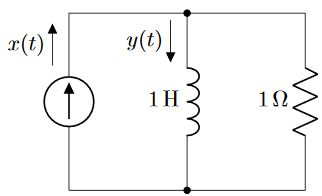
\includegraphics[scale=0.8]{RL.JPG}
        \caption{$RL$电路图}

    \end{figure}

\end{proposition}

\begin{proof}

    \begin{enumerate}

        \item 
            由图可知,$RL$电路的微分方程为
            $$\dfrac{\diff y(t)}{\diff t} + y(t) = x(t)$$
            当输入电流$x(t) = \euler^{-2t}u(t)$,且$y(0^{-}) = 0$时,微分方程的\textup{Laplace}变换为
            $$s\mathscr{Y}(s) + \mathscr{Y}(s) = \mathscr{X}(s) = \dfrac{1}{s + 2}$$
            $$\mathscr{Y}(s) = \dfrac{1}{(s + 1)(s + 2)} = \dfrac{1}{s + 1} - \dfrac{1}{s + 2}$$
            由变换对易知,电路的零状态响应为
            $$y(t) = \euler^{-t}u(t) - \euler^{-2t}u(t)$$
        \item 
            当输入电流$x(t) = 0$,且$y(0^{-}) = 0$时,微分方程的\textup{Laplace}变换为
            $$s\mathscr{Y}(s) - y(0^{-}) + \mathscr{Y}(s) = 0$$
            即
            $$\mathscr{Y}(s) = \dfrac{1}{s + 1}$$
            由\textup{Laplace}变换对易知,电路的零状态响应为
            $$y(t) = \euler^{-t}u(t)$$
        \item 
            当输入电流$x(t) =  \euler^{-2t}u(t)$,初始条件同\textup{(b)}时,
            微分方程的\textup{Laplace}变换为
            $$s\mathscr{Y}(s) - y(0^{-}) + \mathscr{Y}(s) = \mathscr{X}(s) = \dfrac{1}{s + 2}$$
            即
            $$\mathscr{Y}(s) = \dfrac{2}{s + 1}  - \dfrac{1}{s + 2}$$
            由\textup{Laplace}变换对易知,电路的零状态响应为
            $$y(t) = \euler^{-t}u(t) - 2\euler^{-2t}u(t)$$
    \end{enumerate}

    
\end{proof}


\begin{proposition}
    
    关于信号$x(t)$,已知以下三点:
    
    \begin{enumerate}
        \item $x(t) = 0,\ t < 0$
        \item $x\left(\dfrac{k}{80}\right) = 0, \ k = 1, 2, 3, \cdots$
        \item $x\left(\dfrac{1}{160}\right) = \euler^{-120}$
   \end{enumerate}

   设$X(s)$为$x(t)$的\textup{Laplace}变换,则$X(s)$在有限$s$平面内有几个极点。

\end{proposition}

\section{\texorpdfstring{$z$}{z}变换}

\begin{proposition}

    有一个信号$x[n]$的$z$变换的代数表达式为
    $$X(z) = \dfrac{1 + z^{-1}}{1 + \frac{1}{3}z^{-1}}$$

    \begin{enumerate}

        \item 假定收敛域是$|z| > \dfrac{1}{3}$,利用长除法求$x[0]$,$x[1]$和$x[2]$的值。
        \item 假定收敛域是$|z| < \dfrac{1}{3}$,利用长除法求$x[0]$,$x[1]$和$x[2]$的值。
        
    \end{enumerate}

\end{proposition}

\begin{proof}
    
    \begin{enumerate}

        \item 
            $$(1 + z^{-1}) / \left(1 + \frac{1}{3}z^{-1}\right) = \left(1 + \dfrac{2}{3}z^{-1} - \dfrac{2}{9}z^{-2}\right)$$
        \item 
            $$(z^{-1} + 1) / \left(\frac{1}{3}z^{-1} + 1\right) = (3 - 6z^{1} + 18z^{2})$$

    \end{enumerate}

\end{proof}



\end{document}